\documentclass[a4paper,twoside,12pt]{memoir} % jednostrano: promijeniti twoside u oneside

\usepackage[utf8]{inputenc}
\usepackage{diplomski}
% bibliografija na hrvatskom
\usepackage[languagenames,fixlanguage]{babelbib}
% hiperlinkovi
\usepackage[pdftex]{hyperref}
\usepackage{comment}

% Paket graphicx sluzi za manipuliranje grafikom
\usepackage[pdftex]{graphicx}
\graphicspath{ {images/} }
\usepackage{caption}
\captionsetup{justification=centering}
\usepackage{mathtools}
\usepackage{enumitem}
\usepackage{qtree}
\usepackage{float}
\usepackage{ulem}
\usepackage{bm}
\usepackage{csquotes}
\usepackage[usenames,dvipsnames,svgnames,table]{xcolor}

\usepackage{listings}
\usepackage{color}

\definecolor{dkgreen}{rgb}{0,0.6,0}
\definecolor{gray}{rgb}{0.5,0.5,0.5}
\definecolor{mauve}{rgb}{0.58,0,0.82}

\lstset{frame=none,
	language=Java,
	aboveskip=3mm,
	belowskip=3mm,
	showstringspaces=false,
	columns=flexible,
	xleftmargin=-0.5cm,
	basicstyle={\small\ttfamily},
	numbers=none,
	numberstyle=\tiny\color{gray},
	keywordstyle=\color{blue},
	commentstyle=\color{dkgreen},
	stringstyle=\color{mauve},
	breaklines=true,
	breakatwhitespace=true,
	tabsize=3
}
%%%%%
% Singer: Promijenio definiciju \ti, tako da ima 1 argument i doda "italic correction" na kraju argumenta.
%   Prebacio sve \textit u \ti.
%%%%%
%\newcommand{\ti}{\textit}
\newcommand{\ti}[1]{\textit{#1\/}}
\newcommand{\tb}{\textbf}
\newcommand{\ra}{\rightarrow}
\setlist{itemsep=0em}
\pagestyle{headings}


% uz paket fancyhdr mogu se lako kreirati fancy zaglavlja i podnozja

\title{Karakterizacija likova u dje\v cjim pri\v cama}
\author{Gorana Levačić}
\advisor{izv.~prof.~dr.~sc.~Saša Singer}  % obavezno s titulom (prof. dr. sc ili doc. dr. sc.)
\date{studeni, 2016.}  % oblika mjesec, godina

% posveta
%\dedication{Samom sebi}

\begin{document}

	% Naredna frontmatter generira naslovnu stranicu, stranicu za potpise povjerenstva, eventualnu posvetu i sadrzaj
	% Moze se iskomentirati ukoliko nije u pitanju konacna verzija
	\frontmatter

	\begin{intro}

		%%%%%
		% Singer: Uobicajeno je u mnozini, tj. "cemo"
		%%%%%
		%	\textcolor{BrickRed}{Bavit ću se? Bavit ćemo se? Koliko subjektivan i opisan treba biti uvod?}

		U ovom diplomskom radu bavit ćemo se problemom automatske karakterizacije likova u dječjim pričama. Cilj je implementirati jednostavno softversko rješenje koje će, za lika iz dječje priče, s nekom točnošću odrediti je li dobar ili zao. Taj problem pripada području \textbf{obrade prirodnog jezika}, konkretno, razumijevanju prirodnog jezika.

		Problem ćemo pokušati riješiti kombiniranjem nekoliko već razrađenih metoda za obradu prirodnog jezika. Cilj je postojećim alatima analizirati i transformirati tekst u skup podataka koje će računalo znati obraditi. Prvi korak je samo prepoznavanje likova. Taj korak nije nužan, odnosno, možemo sami zadati koji su likovi u priči. Sljedeći korak je razrješavanje koreferencije, odnosno, zamjena svih zamjenica imenima likova na koje se odnose. Naposljetku, za svakog lika možemo automatski izdvojiti rečenice koje se odnose na njega i provesti analizu sentimenta nad njima. Analiza sentimenta će nam dati odgovor na pitanje je li dotičan lik dobar ili zao.

		%%%%%
		% Singer: Zadnja recenica u sljedecem paragrafu?
		%   Smeta me ono "ne bi bio...". Znaci li to da se taj pristup odbacuje?
		%   Fali "Stoga se ogranicavamo na prvi pristup".
		%%%%%
		Drugi mogući pristup se sastoji u oblikovanju i treniranju nekog od modela strojnog učenja nad označenim podacima, odnosno, pričama. Problem ovakvog pristupa je u dostupnosti podataka za učenje. S obzirom da se radi o atipičnom problemu, ne postoji javno dostupan odgovarajući skup podataka. Stoga je, u ovom pristupu, potrebno samostalno stvoriti takav skup. Radi se o čitanju većeg broja priča te ručnom označavanju likova i dijelova rečenica koje se odnose na njihovu ličnost. To je dugotrajan, iscrpljujuć zadatak te postoji vjerojatnost da, na samom kraju, istrenirani model ne bi bio znatno uspješniji od modela dobivenog prvim pristupom.

		Priče su prikupljene s Project Gutenberga, online repozitorija e-knjiga~\cite{gutenberg}. Radi se o dječjim bajkama, poput Crvenkapice ili Snjeguljice. U takvim pričama najčešće imamo svega nekoliko likova koji su strogo podijeljeni na dobre i zle. Stoga su one idealne za rješavanje našeg problema.

		Kako gotovo svi dostupni alati za obradu jezika rade isključivo s engleskim jezikom, dječje priče koje ćemo obrađivati, kao i svi primjeri u ovom diplomskom radu, dani su na engleskom jeziku.

	\end{intro}

	\chapter{Obrada prirodnog jezika}
	%%%%%
	% Singer: Promjenio mark u headeru (izbacio rijeci POGLAVLJE - odurno izgleda).
	%   Nazalost, broj poglavlja moram eksplicitno staviti - pravi brojac je "skriven" u memoir styleu.
	%   Isto sam napravio na svim poglavljima koja imaju broj.
	%%%%%
	\markboth{1. \ OBRADA PRIRODNOG JEZIKA}{}

	\section{Opis područja}

	\textbf{Obrada prirodnog jezika} (eng.~\ti{natural language processing}) je znanstveno područje koje obuhvaća računarstvo, umjetnu inteligenciju i računalnu lingvistiku. Ovom području pripadaju neki od najvažnijih problema iz područja umjetne inteligencije, poput razumijevanja prirodnog jezika, strojnog prevođenja i prepoznavanja govora. S obzirom da je jezik osnovni način sporazumijevanja među ljudima, uspjeh u području obrade prirodnog jezika značio bi ostvarivanje uspješne komunikacije između ljudi i računala.

	%%%%%
	% Singer: Na kraju, dodao  ... recenica (nizova rijeci) danog jezika.
	%%%%%
	Prvi korak u obradi prirodnog jezika je njegovo modeliranje nekim formalnim skupom pravila. U tu svrhu dolazi do oblikovanja formalnih gramatika i semantika. \tb{Formalna gramatika} definira skup pravila za generiranje valjanih rečenica (nizova riječi) danog jezika.

	Opišimo ukratko formalnu gramatiku engleskog jezika. Prvo je potrebno definirati objekte (alfabet) formalne gramatike.
	%%%%%
	% Singer: Dodao promjenu razmaka izmedju recenice i prve stavke u [...].
	%   Razmak stavki (itemsep) je vec na 0. Moze se staviti negativan (itemsep=-0.3ex).
	%%%%%
	% \textcolor{BrickRed}{(previše praznog prostora između stavki, također ovaj razmak između rečenice i prve stavke?)}
	\begin{itemize}[topsep=1.5ex]
		\item	\ti{S (sentence)} --- rečenica
		\item	\ti{NP (noun phrase)} --- imenička fraza, skup riječi koji unutar rečenice čini subjekt ili objekt
		\item	\ti{VP (verb phrase)} --- glagolska fraza, skup riječi koji se unutar rečenice odnosi na predikat
		\item	\ti{PP (prepositional phrase)} --- prepozicijska fraza, skup riječi koji pobliže opisuje neku imenicu ili glagol
		\item	\ti{V} ili \ti{Verb} --- glagol
		\item	\ti{N} ili \ti{Noun} --- imenica
		\item	\ti{Proper-Noun} --- vlastita imenica
		\item	\ti{Pronoun} --- zamjenica
		\item	\ti{Det (determiner)} --- riječ koja pobliže opisuje imenicu na koju se odnosi, na primjer \ti{the, a, this, blue}
		\item	\ti{Prep (preposition)} --- prijedlog
	\end{itemize}
	%%%%%
	% Singer: Ukinuo novi paragraf (praznu liniju).
	%   Dodao \ti za svaku stvar u pravilima - puno bolje izgleda :-)
	%%%%%
	Slijedi nekoliko pravila gramatike engleskog jezika:
	\begin{equation}
	\begin{aligned}
	\ti{S} \rightarrow &\ \ti{NP} \ \ \ti{VP}\\
	\medskip
	\ti{NP} \rightarrow &\ \ti{Pronoun} \\
	& \;\, |\ \ti{Proper-Noun} \\
	& \;\, |\ \ti{Det}\ \ti{Noun}\\
	\medskip
	\ti{VP} \rightarrow &\ \ti{Verb} \\
	& \;\, |\ \ti{Verb}\ \ti{NP}\\
	& \;\, |\ \ti{Verb}\ \ti{NP}\ \ti{PP}\\
	& \;\, |\ \ti{Verb}\ \ti{PP}\\
	\medskip
	\ti{PP} \rightarrow &\ \ti{Prep}\ \ti{NP} \\
	\medskip
	\ti{Prep} \rightarrow& \ \ti{from} \ |\ \ti{to}\ |\ \ti{before}\ |\ \ti{in} \ |\ \ldots\\
	\ti{Verb} \rightarrow& \ \ti{do} \ |\ \ti{eat}\ |\ \ti{look}\ |\ \ti{stay} \ |\ \ldots\\
	\ti{Noun} \rightarrow& \ \ti{girl} \ |\ \ti{cat}\ |\ \ti{bird}\ |\ \ti{forest} \ |\ \ldots\\
	\ti{Pronoun} \rightarrow& \ \ti{I} \ |\ \ti{she}\ |\ \ti{they}\ |\ \ti{someone} \ |\ \ldots\\
	\end{aligned}
	\end{equation}

	Uočimo da se primjenom gornjih pravila rečenice mogu rastaviti na osnovne gramatičke dijelove, ali i obratno --- iz riječi možemo generirati nove gramatički ispravne rečenice. Zbog toga se formalne gramatike zovu i \tb{generativne gramatike}.

	Nadalje, uočimo da gramatička ispravnost ne znači, ujedno, i semantičku ispravnost. Kao primjer, često se navodi rečenica iz~\cite{chomsky},
	%%%%%
	% Singer: prebacio u \displayquote
	%%%%%
	% \ti{"Colorless green ideas sleep furiously."}~\cite{chomsky},
	\begin{displayquote}
		\ti{Colorless green ideas sleep furiously.}
	\end{displayquote}
	koja je gramatički ispravna, ali nema nikakvo smisleno značenje. Iz tog razloga je važno proučavati i semantiku prirodnog jezika. Jedan pristup tome je Montagueva gramatika~\cite{montague1970universal}, koja semantiku prirodnog jezika dovodi u vezu s logikom višeg reda. Dodatno se različitim statističkim metodama modelira semantika prirodnog jezika. Takve metode daju modele koji, za neki niz riječi, predviđaju koliko je vjerojatno da se pojavi u prirodnom jeziku, odnosno, koliko je vjerojatno da je smislen.

	Nažalost, dosad opisani pristupi ne daju sasvim uspješne modele. Razlog tome je izuzetna složenost prirodnog jezika, koja često ljudima nije očita --- kompleksna gramatička pravila, veliki broj iznimaka od tih pravila, višeznačnost riječi i izraza predstavljaju računalima velik problem. Zapravo je nemoguće eksplicitno modelirati čitavu gramatiku i semantiku jednog jezika, te je potrebno promijeniti ili barem nadopuniti ovakav pristup. Kao rješenje se javlja \tb{strojno učenje} (eng.~\ti{machine learning}), koje se krajem prošlog stoljeća počelo snažno razvijati. Svrha strojnog učenja je oblikovati algoritme koji mogu učiti iz podataka te davati predviđanja nad novim podacima. Treniranjem nad velikim skupom podataka računalo može oblikovati odličan model prirodnog jezika, odnosno, njegove strukture, pravila i semantike. Stoga se danas najveći uspjesi, ne samo u obradi prirodnog jezika, već u čitavom području umjetne inteligencije, postižu upravo korištenjem strojnog učenja.

	U nastavku ćemo opisati nekoliko važnijih problema iz ovoga područja vezanih uz problem karakterizacije likova.


	\section{Razumijevanje prirodnog jezika}

	\tb{Razumijevanje prirodnog jezika}  (eng.~\ti{natural language understanding}) je jedan od najvažnijih i najkompleksnijih problema obrade prirodnog jezika. Da bi računalo moglo "razumjeti" tekst, potrebno ga je reprezentirati nekim formalnim jezikom, na primjer, logikom prvog reda. Rješavanje problema otežava činjenica da gotovo svaka rečenica može imati nekoliko mogućih značenja. Često nama (ljudima) neka rečenica ima samo jedno očito značenje, ali računalo može prepoznati i nekoliko desetaka različitih značenja i često neće uspješno odrediti točno značenje. Najčešći razlozi tome su višeznačnost riječi, postojanje frazema i različitih stilskih figura, te nejedinstvenost stabla parsiranja.

	Višeznačnost riječi, pogotovo u engleskom jeziku, potječe iz više izvora. Mnoge engleske riječi u svom izvornom obliku ne pripadaju jednoj, već nekoliko vrsta riječi, te u svakoj od tih vrsta mogu imati više značenja. Na primjer, riječ \ti{iron}, ovisno o kontekstu, može biti imenica, glagol ili pridjev. Značenja imenice \ti{iron} su \ti{željezo}, \ti{glačalo}, ili pak \ti{palica za golf}, dok kao glagol, riječ \ti{iron} ima značenje \ti{glačati}. Pridjev \ti{iron} može značiti \ti{željezni}, ali i \ti{čvrst}, \ti{odlučan}.

	Uz višeznačnost riječi je vezan i pojam \ti{frazema}. Frazemi, u engleskom jeziku poznatiji kao \ti{idiomi}, su višečlane jezične jedinice koje se uvijek javljaju kao cjelina te im je stvarno značenje različito od doslovnog značenja tog niza riječi. Ispuštanje ili zamjena samo jedne riječi u frazemu dovodi do gubljenja njegovog značenja. Na primjer, engleski idiom \ti{piece of cake} označava jednostavnu i laganu aktivnost, zadatak ili posao. Analogni hrvatski frazem bi bio \ti{mačji kašalj}. U oba slučaja očito je da frazem ima posve različito značenje od doslovnog značenja. U rečenici poput
	%%%%%
	% Singer: prebacio u \displayquote
	%%%%%
	% \ti{"The exam was piece of cake."},
	\begin{displayquote}
		\ti{The exam was piece of cake.}
	\end{displayquote}
	čovjeku je očito da se radi o figurativnom značenju. S druge strane, u nekim situacijama će riječi, koje inače čine frazem, imati svoje doslovno značenje, kao u rečenici:
	%%%%%
	% Singer: prebacio u \displayquote
	%%%%%
	% \ti{"I went on her birthday party and ate large piece of cake."}.
	\begin{displayquote}
		\ti{I went on her birthday party and ate large piece of cake.}
	\end{displayquote}

	\bigskip

	Posljednji razlog tomu što računala najčešće prepoznaju više značenja iste rečenice je taj, što se za istu rečenicu može izgraditi više \ti{stabala parsiranja}. Stablo parsiranja predstavlja gramatičku strukturu rečenice. Pogledajmo dva moguća stabla parsiranja za poznatu rečenicu iz filma \ti{Animal Crackers} braće Marx:
	%%%%%
	% Singer: prebacio u \displayquote
	%%%%%
	% \ti{"I shot an elephant in my pajamas."}
	\begin{displayquote}
		\ti{I shot an elephant in my pajamas.}
	\end{displayquote}
	Oznake čvorova su definirane u prethodnoj sekciji.

	\begin{figure}[H]
		\Tree
		[.\ti{S}
		[.\ti{NP} [\ti{I} ]]
		[.\ti{VP}
		[.\ti{VP}
		[.\ti{V} [\ti{shot} ]]
		[.\ti{NP}
		[.\ti{Det} [\ti{an} ]]
		[.\ti{N} [\ti{elephant} ] ]
		]
		]
		[.\ti{PP}
		[.\ti{P} [\ti{in} ]]
		[.\ti{NP}
		[.\ti{Det} [\ti{my} ]]
		[.\ti{N} [\ti{pajamas} ]]
		]
		]
		]
		]
	\end{figure}

	\noindent
	Ovo stablo parsiranja odgovara značenju
	%%%%%
	% Singer: prebacio u \displayquote
	%%%%%
	% \ti{"I was in my pajamas when I shot the elephant."}.
	\begin{displayquote}
		\ti{I was in my pajamas when I shot the elephant.}
	\end{displayquote}
	%%%%%
	% Singer: Dodao skok na novu stranicu - bolje nego da "razvlaci" razmake do dna stranice (zbog "twoside").
	%%%%%
	\newpage

	\begin{figure}[H]
		\Tree
		[.\ti{S}
		[.\ti{NP} [\ti{I} ]]
		[.\ti{VP}
		[.\ti{V} [\ti{shot} ]]
		[.\ti{NP}
		[.\ti{Det} [\ti{an} ]]
		[.\ti{N} [\ti{elephant} ] ]
		[.\ti{PP}
		[.\ti{P} [\ti{in} ]]
		[.\ti{NP}
		[.\ti{Det} [\ti{my} ]]
		[.\ti{N} [\ti{pajamas} ]]
		]
		]
		]
		]
		]
	\end{figure}

	\noindent
	S druge strane, ovo stablo parsiranja odgovara značenju
	%%%%%
	% Singer: prebacio u \displayquote
	%%%%%
	% \ti{"I shot the elephant which was wearing my pajamas."}.
	\begin{displayquote}
		\ti{I shot the elephant which was wearing my pajamas.}
	\end{displayquote}

	\bigskip

	Uočimo da još ne možemo prevesti ovu rečenicu na hrvatski jezik, jer nam nije poznato značenje riječi \ti{shot}. Naime, možemo ju shvatiti kao \ti{upucati} (puškom tijekom lova) ili kao \ti{fotografirati}. Tek uz kontekst možemo točno interpretirati značenje:
	%%%%%
	% Singer: prebacio u \displayquote
	%%%%%
	% \ti{"While hunting in Africa, I shot an elephant in my pajamas. How he got into my pajamas, I don't know."}.
	\begin{displayquote}
		\ti{While hunting in Africa, I shot an elephant in my pajamas. How he got into my pajamas, I don't know.}
	\end{displayquote}


	\section{Prepoznavanje imenovanih entiteta}

	\tb{Prepoznavanje imenovanih entiteta} (eng.~\ti{named entity recognition}, skraćeno NER) je problem određivanja i klasifikacije onih fraza u tekstu koje se odnose na osobe, lokacije, organizacije i druge istaknute pojmove. Zajednički naziv za takve fraze je \tb{imenovani entitet} (eng.~\ti{named entity}). Drugim riječima, imenovani entitet definiramo kao objekt stvarnog svijeta koji ima vlastito ime. Pogledajmo primjer:

	\bigskip

	%%%%%
	% Singer: Ovo namjerno NISAM prebacio u \displayquote, jer javlja overfull \hbox!
	%%%%%
	\ti{The girl called $\underbracket{\text{Red Riding Hood}}_{\text{Person}}$ walked through the forest called $\underbracket{\text{Grünewald}}_{\text{Location}}$.}

	\bigskip

	Uočimo da se NER problem sastoji od dva problema --- prepoznavanja samih entiteta (\ti{Red Riding Hood}) i njihovog svrstavanja u unaprijed poznate kategorije (\ti{Person}). Stoga se naivni pristup rješavanju problema sastoji od dva koraka. Prvi korak je označiti kao imenovani entitet sve riječi pisane velikim početnim slovom. Problem prvog koraka je u tome što prva riječ svake rečenice, također, započinje velikim slovom. S druge strane, često naziv entiteta sadrži riječi pisane malim početnim slovom, kao što je u slučaju \ti{Hrvatske narodne banke}. Nadalje, arapski i kineski jezik uopće nemaju kapitalizaciju, dok se u njemačkom jeziku sve imenice pišu velikim početnim slovom, pa se ovakav pristup uopće ne može primijeniti.

	Drugi korak naivnog pristupa bi se sastojao u definiranju skupa svih entiteta neke kategorije, npr.\ \ti{location} $= \{\ti{Zagreb}, \ti{Rijeka}, \ti{Velebit}, \ldots\}$, nakon čega bismo za pronađene entitete provjeravali nalaze li se u nekoj od kategorija. Osim što je nemoguće popisati sve moguće entitete (npr.\ sva ljudska imena), problem je i višeznačnost teksta --- \ti{Irska} može, ovisno o kontekstu, označavati državu ili otok.

	Iz prethodno opisanih problema zaključujemo da je prepoznavanju entiteta potrebno pristupiti metodama strojnog učenja. U sljedećem poglavlju ćemo formalno opisati danas najčešće korištene metode rješavanja NER problema.

	\bigskip

	Za sam kraj ovog dijela opišimo vezu problema prepoznavanja imenovanih entiteta i karakterizacije likova u dječjim pričama.
	Svi dostupni sustavi, kao što je \ti{Stanford NER}, prepoznaju barem kategorije \ti{Person}, \ti{Location}, \ti{Organisation}. Kod problema karakterizacije dobrih i loših likova, u priči je dovoljno prepoznati samo jednu kategoriju entiteta --- likove. Očito je da su, najčešće, sve (imenovane) osobe spomenute u priči, ujedno i likovi. Obrat ne vrijedi --- nisu svi likovi (imenovane) osobe. Na primjer, uz Snjeguljicu se u istoimenoj bajki javljaju lovac i zla kraljica. Oni su očito likovi, ali kako nisu posebno imenovani, nijedan postojeći NER sustav ih neće prepoznati i klasificirati kao osobe (\ti{Person}). Zato je potrebno istrenirati novi model koji će prepoznavati sve likove, neovisno o njihovom imenu.


	\section{Razrješavanje koreferencije}

	Problem \tb{razrješavanja koreferencije}  (eng.~\ti{coreference resolution}) čini prepoznavanje onih izraza u tekstu koji se odnose na isti izvanjezični entitet. Koreferentni izrazi mogu biti različitih oblika, kao što su vlastita imena, imeničke fraze ili zamjenice. Razlikujemo više vrsta koreferencije te ih dijelimo na zamjeničke i imeničke. Anafora, katafora i podijeljeni prethodnici su primjer zamjeničke koreferencije, dok koreferirajuće imeničke fraze pripadaju imeničkoj koreferenciji.

	%%%%%
	% Singer: Bold je na mjestu.
	%   Oko boja: ako izgleda prekicasto, mogu se koristiti razne crste "podvlacenje" iz "ulem" paketa.
	%   Na pr.:  \uvawe za zamjenicu, \uline za izraz (promijeniti onda i u tekstu - "podcrtana valovitom crtom", "podcrtan ravnom crtom").
	%%%%%
	%	\textcolor{BrickRed}{Koristiti boje za ovaj naglasak? Ili nešto drugo? Malo mi se čini kičasto, bold, boje... Prije su anafora, katafora, koref. imen. fraze, pod. prethodnici bili italic.}

	\tb{Anafora} označava koreferenciju u kojoj se zamjenica (napisana plavom bojom) javlja nakon izraza na kojeg se referira (izraz je napisan crvenom bojom). Jasnije je iz primjera:
	%%%%%
	% Singer: prebacio u \displayquote
	%%%%%
	% \ti{"\textcolor{BrickRed}{Red Riding Hood} was so happy that \textcolor{Blue}{she} wanted to dance through the forest."}
	\begin{displayquote}
		\ti{\textcolor{BrickRed}{Red Riding Hood} was so happy that \textcolor{Blue}{she} wanted to dance through the forest.}
	\end{displayquote}

	\smallskip

	S druge strane, \tb{katafora} označava koreferenciju u kojoj se zamjenica javlja prije izraza na kojeg se referira:
	%%%%%
	% Singer: prebacio u \displayquote
	%%%%%
	% \ti{"\textcolor{Blue}{She} always wore red cloak with a hood, so people called \textcolor{Blue}{her} \textcolor{BrickRed}{Little Red Riding Hood}."}
	\begin{displayquote}
		\ti{\textcolor{Blue}{She} always wore red cloak with a hood, so people called \textcolor{Blue}{her} \textcolor{BrickRed}{Little Red Riding Hood}.}
	\end{displayquote}

	\smallskip

	I anafora i katafora mogu uključivati \tb{podijeljene prethodnike}. Radi se o obuhvaćanju više riječi jednom zamjenicom:
	%%%%%
	% Singer: prebacio u \displayquote
	%%%%%
	% \ti{"When \textcolor{BrickRed}{Little Red Riding Hood} and \textcolor{BrickRed}{the wolf} met, \textcolor{Blue}{they} spoke as old friends."}
	\begin{displayquote}
		\ti{When \textcolor{BrickRed}{Little Red Riding Hood} and \textcolor{BrickRed}{the wolf} met, \textcolor{Blue}{they} spoke as old friends.}
	\end{displayquote}

	\smallskip

	Posljednja vrsta koreferencije koju ćemo navesti su \tb{koreferirajuće imeničke fraze}. Ona označava referiranje na neku imeničku frazu drugom imeničkom frazom:
	%%%%%
	% Singer: prebacio u \displayquote
	%%%%%
	% \ti{"\textcolor{Blue}{The girl in red riding hood} was so happy on that sunny day. \textcolor{BrickRed}{The child} was singing merrily while walking through the forest."}
	\begin{displayquote}
		\ti{\textcolor{Blue}{The girl in red riding hood} was so happy on that sunny day. \textcolor{BrickRed}{The child} was singing merrily while walking through the forest.}
	\end{displayquote}

	\smallskip

	U zasebnom poglavlju opisat ćemo nekoliko metoda koje se koriste za razrješavanje koreferencije.


	\section{Analiza sentimenta}

	Također poznata i pod nazivom \tb{rudarenje stavova} (eng.~\ti{opinion mining}), \tb{analiza sentimenta} (eng.~\ti{sentiment analysis}) bavi se identificiranjem i ekstrakcijom subjektivnih informacija u tekstu. Najčešće se primjenjuje nad recenzijama, komentarima i kritikama objavljenim na različitim društvenim medijima, a u svrhu marketinga ili poboljšanja usluge.

	Osnovni i najčešći zadatak analize sentimenta je određivanje polariteta danog teksta, odnosno, prepoznavanje stava izrečenog u tekstu kao pozitivnog, negativnog ili neutralnog. Osim toga, analiza sentimenta za cilj može imati i klasifikaciju teksta na objektivni ili subjektivni. Najkompleksniji oblik analize sentimenta se odnosi na više karakteristika objekta o kojemu se u tekstu govori. Tada je cilj raspoznati koje karakteristike su ocijenjene pozitivno, a koje negativno. Na primjer, korisnička recenzija nekog proizvoda može uključivati pohvale za dizajn, ali i negativne kritike o cijeni.

	\bigskip

	%%%%%
	% Singer: Okrenuo poredak rijeci u prvoj recenici.
	%%%%%
	%	Najčešće po prisutnosti nekih riječi možemo prepoznati polaritet teksta ili rečenice.
	Polaritet teksta ili rečenice najčešće možemo prepoznati po prisutnosti nekih riječi. Na primjer, ako se u rečenici spominju negativne riječi, poput pridjeva \ti{evil}, \ti{selfish}, glagola \ti{hate} ili imenice \ti{junk}, sentiment je vjerojatno negativan. S druge strane, ako se koriste pozitivne riječi, kao što su pridjevi \ti{great}, \ti{nice}, glagoli \ti{love}, \ti{like} ili imenica \ti{delight}, možemo zaključiti da je sentiment pozitivan.

	\begin{displayquote}
		\ti{This story is interesting and it has good characters and good ending.}
	\end{displayquote}

	Ipak, često nije dovoljno promatrati isključivo riječi u tekstu. Naime, u neutralnim rečenicama se mogu javiti i pozitivne riječi, kao u sljedećem slučaju:
	%%%%%
	% Singer: \displayquote je OK, ali bih ga poceo koristiti i ranije - bilo je takvih stvari i prije!
	%   Dodao ranije, svagdje gdje mi dobro izgleda!
	%%%%%
	%	\textcolor{BrickRed}{Displayquote je ok? Neki drugi način naglašavanja, tj. davanja primjera? Enumitem bez oznake?}
	\begin{displayquote}
		\ti{Is this story interesting? Does it have good characters and good ending?}
	\end{displayquote}

	Nadalje, velik problem predstavlja oblik predikata, što može u potpunosti promijeniti značenje teksta. Jednak utjecaj ima i prisutnost nekih riječi ili izraza, poput \ti{not}, \ti{any}, \ti{at all}. Na primjer, sljedeće rečenice su posve suprotnog polariteta, iako im je građa gotovo jednaka:
	\begin{displayquote}
		\ti{I heard this book was brilliant. In the end, I was disappointed.}\\
		\ti{I heard this book was brilliant. In the end, I wasn't disappointed at all.}
	\end{displayquote}

	U sljedećem primjeru oblik predikata određuje stav. U prvom slučaju radi se o negativnom stavu --- knjiga je \ti{trebala biti} odlična, ali očito nije. Druga rečenica je jasno pozitivnog stava:
	\begin{displayquote}
		\ti{This book was supposed to be brilliant.}\\
		\ti{This book is brilliant.}
	\end{displayquote}

	Još veći problem predstavlja sarkazam, odnosno, rečenica koja je po smislu pozitivna, ali ju treba shvatiti negativno. Često je i ljudima teško prepoznati sarkazam u tekstu. U sljedećem primjeru prvu rečenicu treba shvatiti sarkastično, odnosno, kao negativnu, dok druga ima doslovno, pozitivno značenje. Naglašene riječi su podcrtane.
	\begin{displayquote}
		\ti{I \underline{can't wait} to see that old lady, she is \underline{so} nice.}\\
		\ti{I can't wait to see that old lady, she is so nice.}
	\end{displayquote}

	Također je problematično prepoznati sentiment u rečenicama u kojima, nao\-či\-gled, nema niti negativnih niti pozitivnih riječi. Na primjer, u sljedećem slučaju možemo se složiti da je vila učinila loše djelo:
	\begin{displayquote}
		\ti{Old fairy left the children to wander alone in endless forest.}
	\end{displayquote}

	Jedini način kako prepoznati sentiment takvog teksta je shvatiti njegovo zna\-če\-nje, odnosno, utvrditi bit tvrdnje koja se izriče. To je više problem razumijevanja prirodnog jezika, nego klasične analize sentimenta.

	\bigskip

	Neke od metoda koje se koriste u analizi sentimenta ćemo detaljnije opisati u zasebnom poglavlju.


	\chapter{Modeli za prepoznavanje imenovanih entiteta}

	\markboth{2. \ MODELI ZA PREPOZNAVANJE IMENOVANIH ENTITETA}{}

	\section{Generativni i diskriminativni modeli}

	Za početak, opisat ćemo dvije velike klase modela kojima pripadaju danas najčešće korišteni modeli za prepoznavanje imenovanih entiteta. To su generativni i diskriminativni modeli.

	\bigskip

	Neka je $X$ skup ulaznih varijabli te $Y$ skup izlaznih varijabli. U slučaju prepoznavanja imenovanih entiteta, $X$ može uključivati podatke kao što su broj, rod i vrsta riječi, dok $Y$ sadrži informaciju o kategorijama kojima pripada svaka riječ nekog izraza u tekstu. Varijable skupa $X$ promatramo, dok varijable skupa $Y$ želimo predvidjeti sa što većom točnošću.

	Neka su dani vektor ulaznih varijabli $\mathbf{x} \in X$ i izlazni vektor $\mathbf{y} \in Y$. Prepoznati imenovane entitete u suštini znači odabrati niz riječi za koje je vjerojatnost $\mathbb{P}(\mathbf{x}, \mathbf{y})$ dovoljno visoka.

	\bigskip

	Prisjetimo se, za dvije varijable $X$ i $Y$ vrijedi Bayesovo pravilo:
%%%%%
% Singer: LaTeX i AMSLaTeX kazu da ispred jednadzbe NE smije prazna linija.
%   Ukinuo praznu liniju na ovom mjestu.
%%%%%
	\begin{equation}
	\begin{split}
	\mathbb{P}(Y=y, X=x) &= \mathbb{P}(X=x) \cdot \mathbb{P}(Y=y | X=x) \\
	&= \mathbb{P}(Y=y) \cdot \mathbb{P}(X=x | Y=y).
	\end{split}\label{bayes_rule}
	\end{equation}

	Dakle, za modeliranje zajedničke distribucije varijabli $X$ i $Y$ je potrebno znati distribuciju $\mathbb{P}(X)$. Analogno, u slučaju vektora $\mathbf{x}$, radi se o distribuciji $\mathbb{P}(\mathbf{x})$. S obzirom da varijable vektora $\mathbf{x}$ mogu uključivati kompleksne međuzavisnosti, često nije moguće odrediti njegovu distribuciju. U slučaju kada je to moguće, dobiveni model može biti prekompleksan za izračunavanje. S druge strane, ignoriranje međuzavisnosti često rezultira lošim ili čak neupotrebljivim modelom.

	Ovakvi modeli zajedničke distribucije se nazivaju \tb{generativni modeli}. Naziv je intuitivan --- oni izravno opisuju kako vrijednosti ulaznih varijabli (probabilistički) generiraju vrijednost izlaznih. Stoga se generativni modeli mogu koristiti i za generiranje novih podataka.

	S druge strane, \tb{diskriminativni modeli} su modeli uvjetne distribucije $\mathbb{P}(\mathbf{y}|\mathbf{x})$. Oni ne zahtijevaju modeliranje distribucije $\mathbb{P}(\mathbf{x})$. U praksi, $\mathbb{P}(\mathbf{x})$ često nije niti potrebna za rješavanje danog problema. U našem slučaju, nije bitno je li međusobno povezan rod imenice i njezino završno slovo, već samo koliko je vjerojatno da ta imenica pripada zadanoj klasi uz dani ulaz. Zato se često diskriminativnim modelima postižu puno bolji rezultati.

	Zanimljiva je činjenica da postoji međusobna uparenost generativnih i diskriminativnih modela. To znači da su dva modela oblikovana nad istim prostorom hipoteza te da učenjem nad jednakim podacima daju jednaki rezultat. Iz toga slijedi da se generativni model može preinačiti u diskriminativni i obratno. O tome ćemo detaljnije reći nakon što damo neke primjere modela.


	\section{Grafički modeli}

	Grafički modeli su statistički modeli koji se uobičajeno koriste za prikaz ovisnosti među varijablama. Jedan model čini skup vjerojatnosnih distribucija koje se faktoriziraju prema definiranom grafu. Cilj grafičkih modela je prikazati distribuciju nad velikim brojem slučajnih varijabli kao produkt lokalnih funkcija manjeg broja varijabli.

	\bigskip

	Neka su $X = \{x_1, \ldots, x_n\}$ skup ulaznih varijabli koje promatramo i $Y = \{y_1, \ldots, y_m\}$ skup izlaznih varijabli koje želimo predvidjeti. Nadalje, neka je $V = X \cup Y$. Svaki $v \in V$ poprima vrijednosti iz nekog skupa $\mathcal{V}$. Neka su dani ulazni vektor $\mathbf{x} \in X$  i izlazni vektor $\mathbf{y} \in Y$ . Za dani podskup $A \subseteq V$, s $\mathbf{x}_A$ označavamo vektor ulaznih varijabli takvih da je $x_i \in A$. Analogno, s $\mathbf{y}_A$ označavamo vektor izlaznih varijabli za koje je $y_j \in A$.

	\begin{defn}
		Neka je $\mathcal{F}$ familija nekih podskupova $A \subseteq V$. \tb{Neusmjereni grafički model} je skup svih distribucija koje se mogu zapisati u obliku
		\begin{equation}\label{graph_distr}
		\mathbb{P}(\mathbf{x}, \mathbf{y}) = \frac{1}{Z} \prod_{A \in \mathcal{F}} \Psi_{A} (\mathbf{x}_A, \mathbf{y}_A),
		\end{equation}
		za neki izabrani skup funkcija $F = \{\Psi_A\}$, pri čemu su $\Psi_A : \mathcal{V}^{|A|} \to \mathbb{R}^+$.

		\medskip

		Elemente skupa $F$ nazivamo \tb{faktorima} ili \tb{lokalnim funkcijama}. Konstantu $Z$ nazivamo \tb{normalizacijski faktor} i definiramo kao
		\begin{equation*}
		Z = \sum_{\mathbf{x}, \mathbf{y}} \prod_{A} \Psi_{A} (\mathbf{x}_A, \mathbf{y}_A).
		\end{equation*}
	\end{defn}

	Normalizacijski faktor osigurava da distribucija ima sumu jednaku jedan, odnosno, da vrijedi
	\begin{equation*}
	\sum\limits_{\mathbf{x}, \mathbf{y}} \mathbb{P}(\mathbf{x}, \mathbf{y}) = 1.
	\end{equation*}

	S obzirom da se u gornjem izrazu sumira po svim mogućim vrijednostima vektora $\mathbf{x}$ i $\mathbf{y}$, u praksi je, najčešće, faktor $Z$ nemoguće izračunati. Stoga se koriste različite metode za njegovu aproksimaciju.

	\bigskip

	Faktorizaciju \eqref{graph_distr} grafički prikazujemo faktor grafom.

	\begin{defn}\label{factor_graph}
		\tb{Faktor graf} za distribuciju vjerojatnosti \eqref{graph_distr} je bipartitni graf $G = (V,F,E)$, pri čemu je čvor-varijabla $v \in V$ povezan s čvorom-faktorom $\Psi_{A} \in F$ ako i samo ako je $v$ argument funkcije $\Psi_{A}$.
	\end{defn}

	\bigskip

	Uz faktor grafove, postoje i druge vrste grafičkih modela. Najjednostavniji od njih su usmjereni grafički modeli. Oni se prikazuju usmjerenim acikličkim grafom $G = (V,E)$.

	\begin{defn}
		\tb{Usmjereni grafički model} ili \tb{Bayesova mreža} se definira kao zajednička distribucija vjerojatnosti koja se faktorizira kao
		\begin{equation*}
		\mathbb{P}( \mathbf{x}, \mathbf{y}) = \prod_{v \in V}\mathbb{P}(v|\pi(v)),
		\end{equation*}
		gdje su $\pi(v)$ roditelji čvora $v$ u grafu $G$.
	\end{defn}

	Usmjereni grafički modeli se mogu koristiti za prikazivanje generativnih modela. Konkretno, generativni modeli se prikazuju usmjerenim modelima u kojima izlazne varijable uvijek prethode ulaznima. Drugim riječima, nijedna ulazna varijabla $x \in X$ ne može biti roditelj izlaza $y \in Y$.

	\bigskip

	Prije nego damo primjere grafičkih modela, opisat ćemo dva jednostavna modela za klasifikaciju. Nakon toga ćemo pokazati kako se oni proširuju do modela koji se, između ostalog, koriste za rješavanje problema imenovanih entiteta.

	\section{Klasifikacija}

	\tb{Klasifikacija} (eng.~\ti{classification}) je problem predviđanja klase varijable $y$ na temelju ulaznog vektora značajki $\mathbf{x} = (x_1, \ldots, x_n)$. Na primjer, u slučaju određivanja spola nekog lika $y$ u priči, (uobičajene) klase su \ti{muško, žensko}. Neke od značajki mogu biti \ti{završno slovo imena, završni slog imena, zamjenica koja se koristi pri referiranju na lika} i slično.

	Dva poznata klasifikatora, odnosno, modela koji rješavanju ovaj problem, su naivni Bayesov klasifikator i logistička regresija.

	\bigskip

	\tb{Naivni Bayesov klasifikator} (eng.~\ti{naive Bayes classifier}) koristi pretpostavku da su, ukoliko je poznata klasa, sve značajke međusobno nezavisne. Očito je da u stvarnom svijetu ne vrijedi nezavisnost. Unatoč tome, u praksi naivni Bayesov klasifikator pokazuje dosta dobre rezultate. Također, iz njegove jednostavnosti slijedi velika brzina, lakoća implementacije i niska potreba za računalnim resursima. Iz navedenih razloga se naivni Bayesov klasifikator često koristi za rješavanje mnogih problema, poput detekcije spam poruka, analize sentimenta ili automatske medicinske dijagnoze.

	\begin{defn}
		\tb{Naivni Bayesov klasifikator} je zajednička distribucija vjerojatnosti koja se faktorizira kao
		\begin{equation} \label{naive_bayes}
		\mathbb{P}(y, \mathbf{x}) = \mathbb{P}(y) \prod_{i=1}^{n}\mathbb{P}(x_i|y).
		\end{equation}
	\end{defn}

	Model je moguće prikazati usmjerenim grafičkim modelom ili faktor grafom.

	\begin{figure}[H]
		\centering
		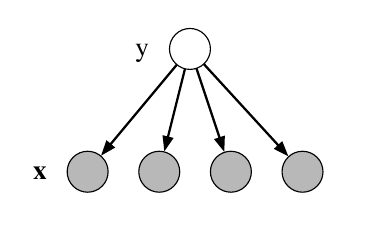
\includegraphics[scale = 0.5]{bayes_directed.png}
		\caption{Naivni Bayesov klasifikator kao usmjereni grafički model}
	\end{figure}

	Ukoliko model prikazujemo faktor grafom, faktori su dani s $\Psi(y) = \mathbb{P}(y)$ te $\Psi_i(y, x_i) = \mathbb{P}(x_i|y)$, za svaki $x_i$. Dogovorno, krugovi označavaju čvorove-varijable, a kvadrati čvorove-faktore.

	\begin{figure}[H]
		\centering
		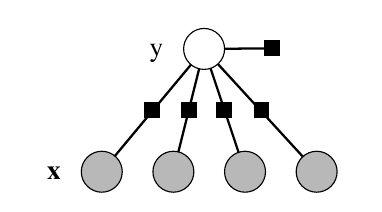
\includegraphics[scale = 0.5]{bayes_factor_graph.png}
		\caption{Naivni Bayesov klasifikator kao faktor graf}
	\end{figure}

	Drugi često korišteni klasifikator je \tb{logistička regresija} (eng.~\ti{logistic regression}). Klasifikator polazi od pretpostavke da je logaritam vjerojatnosti svake klase, $\log(\mathbb{P}(y|\mathbf{x}))$, linearna funkcija od $\mathbf{x}$ (uz normalizacijsku konstantu).

	\begin{defn} \tb{Logistička regresija} je uvjetna distribucija vjerojatnosti koja se faktorizira kao
		\begin{equation*}
		\mathbb{P}(y|\mathbf{x}) = \frac{1}{Z(\mathbf{x})} \exp \bigg(\sum_{i=1}^{n} \theta_i f_i(y, \mathbf{x})\bigg),
		\end{equation*}
		pri čemu su $\theta_i \in \mathbb{R}$ parametri, $f_i$ funkcije koje nazivamo \tb{funkcije značajki}, dok je $Z(\mathbf{x})$ normalizacijska konstanta definirana s
		\begin{equation*}
		Z(\mathbf{x}) = \sum_{\tilde{y},\tilde{\mathbf{x}}} \exp \bigg(\sum_{i=1}^{n} \theta_i f_i(\tilde{y}, \tilde{\mathbf{x}})\bigg).
		\end{equation*}
	\end{defn}

	Logistička regresija se prikazuje faktor grafom:

	\begin{figure}[H]
		\centering
		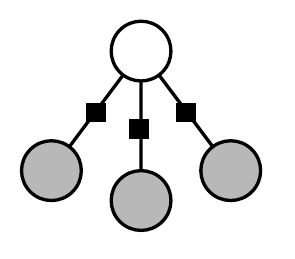
\includegraphics[scale = 0.35]{logistic.png}
		\caption{Prikaz logističke regresije kroz faktor graf}
	\end{figure}

	Naivni Bayesov klasifikator i logistička regresija čine generativno--dis\-kri\-mi\-na\-tiv\-ni par. Naime, ukoliko u logističkoj regresiji maksimiziramo zajedničku vjerojatnost
	\begin{equation*}
	\mathbb{P}(y, \mathbf{x}) = \frac{1}{Z(\mathbf{x})} \exp \bigg(\sum_{i=1}^{n} \theta_i f_i(y, \mathbf{x})\bigg),
	\end{equation*}
	dobivamo onaj klasifikator kojega generira naivni Bayes.

	Obratno, upotrebom Bayesovog pravila \eqref{bayes_rule} nad Bayesovim klasifikatorom \eqref{naive_bayes} dobivamo diskriminativni model
	\begin{equation*}
	\mathbb{P}(y | \mathbf{x}) = \frac{\mathbb{P}(y, \mathbf{x})} {\mathbb{P}(\mathbf{x})} = \frac{\mathbb{P}(y) \prod_{i=1}^{n}\mathbb{P}(x_i|y)} {\mathbb{P}(x_1, \ldots, x_n)}.
	\end{equation*}
	Ovakav klasifikator generira i logistička regresija.


	\section{Skriveni Markovljevi modeli}

	\tb{Skriveni Markovljevi modeli} (eng.~\ti{hidden Markov models}, kraće HMM) čine svojevrsnu nadogradnju naivnog Bayesovog klasifikatora na model koji, umjesto za jednu varijablu, odlučuje za vektore varijabli. Objasnimo kako je došlo do te nadogradnje.

	Neka je dan neki niz riječi (tekst) u kojem želimo prepoznati imenovane entitete nekih kategorija, na primjer, \ti{Osoba}, \ti{Lokacija}, \ti{Organizacija}. Uobičajeno se uvodi oznaka \ti{Ostalo}, koja označava da riječ nije dio imenovanog entiteta. Jedan od pristupa rješavanju NER problema je nezavisno klasificiranje svake riječi niza nekom od navedenih oznaka. Problem koji se pri tome javlja je upravo pretpostavljena nezavisnost. S obzirom da imenovani entiteti često sadrže više riječi, očito imamo zavisnost među tim riječima. Na primjer, \ti{New York} označava lokaciju, dok je \ti{New York Times} organizacija.

	Skriveni Markovljevi modeli djelomično relaksiraju pretpostavku o neovisnosti. HMM modelira ulazni niz $\mathbf{x} = \{x_1, \ldots, x_T\}$ tako da pretpostavlja postojanje niza stanja $\mathbf{y} = \{y_1, \ldots, y_T\}$ koja odgovaraju nizu $\mathbf{x}$. U našem slučaju, $x_t$ označava riječ na poziciji $t$, dok je $y_t$ oznaka kategorije pridjeljene riječi $x_t$. Pri modeliranju zajedničke distribucije $\mathbb{P}(\mathbf{y}, \mathbf{x})$ koriste se dvije pretpostavke o nezavisnosti.

	Prvo pretpostavljamo da svaka oznaka $y_t$ ovisi jedino o svom neposrednom prethodniku $y_{t-1}$, odnosno, da ne ovisi o ostalim prethodnicima $y_{t-2}, \ldots, y_1$. Formalni zapis ove pretpostavke glasi:
	\begin{equation*}
	\mathbb{P}(y_t=y'_t \mid y_{t-1} = y'_{t-1}, \ldots, y_1 = y'_1) = \mathbb{P}(y_t=y'_t \mid y_{t-1} = y'_{t-1}),
	\end{equation*}
	pri čemu je $y'_j$ vrijednost oznake $y_j$, odnosno, neka od vrijednosti \ti{Osoba}, \ti{Lokacija}, \ti{Organizacija}, \ti{Ostalo}. Ovo svojstvo se naziva \tb{Markovljevo svojstvo}.

	Druga pretpostavka je ta da svaka varijabla $x_t$ ovisi isključivo o trenutnoj kategoriji $y_t$. Odavde potječe naziv \ti{skriveni} Markovljevi modeli. Ulaz nije izravno vidljiv, već je vidljiv samo rezultat koji ovisi o tom ulazu.

	Koristimo tri distribucije vjerojatnosti da bismo definirali skriveni Markovljev model. Prva je distribucija početnih oznaka $\mathbb{P}(y_0)$, odnosno, oznaka koje nemaju prethodnika. Sljedeća je distribucija prijelaza $\mathbb{P}(y_t|y_{t-1})$. Osim što je $t$ indeks pojedine riječi u nizu, on označava i indeks pojedinih prijelaza za zadani izlazni vektor.
	Posljednja distribucija, $\mathbb{P}(x_t|y_t)$, opisuje vezu ulazne i izlazne varijable.

	Ove distribucije će biti jasnije iz primjera. Neka je dan ulazno-izlazni par vektora $\mathbf{x}$ i $\mathbf{y}$, odnosno, rečenice i ispravnih oznaka za tu rečenicu:
	\begin{align*}
	\mathbf{x} &= \text{\ti{Red}, \ti{Riding}, \ti{Hood}, \ti{walked}, \ti{through}, \ti{Grünewald}},\\
	\mathbf{y} &= \text{\ti{Osoba}, \ti{Osoba}, \ti{Osoba}, \ti{Ostalo}, \ti{Ostalo}, \ti{Lokacija}}.
	\end{align*}

	Distribucija početnih oznaka opisuje vjerojatnost da prva riječ u rečenici pripada klasi \ti{Osoba}. Distribucija prijelaza opisuje vjerojatnost da, na primjer, nakon oznake \ti{Lokacija} slijedi oznaka \ti{Osoba} (niska vjerojatnost), odnosno, \ti{Lokacija} ili \ti{Ostalo} (visoka vjerojatnost). Posljednja navedena distribucija opisuje vjerojatnost da je ulazna riječ bila \ti{Grünewald} ako je izlaz \ti{Lokacija}.

	Sada možemo dati formalnu definiciju skrivenih Markovljevih modela.

	\begin{defn}
		Neka su $\mathbf{x} = \{x_1, \ldots, x_T\}$ i $\mathbf{y} = \{y_1, \ldots, y_T\}$ slučajni vektori. \tb{Skriveni Markovljev model} je zajednička distribucija vjerojatnosti oblika
		\begin{equation*}
		\mathbb{P}(\mathbf{y}, \mathbf{x}) = \prod_{t=1}^{T} \mathbb{P}(y_t | y_{t-1}) \mathbb{P}(x_t | y_t),
		\end{equation*}
		pri čemu smo za $\mathbb{P}(y_1)$ koristili zapis $\mathbb{P}(y_1 | y_0)$.
	\end{defn}

	Skriveni Markovljevi modeli se mogu prikazati usmjerenim grafom, kao na sljedećoj slici:

	\vspace*{-6pt}
	\begin{figure}[H]
		\centering
		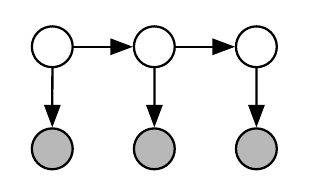
\includegraphics[scale = 0.5]{hmm.png}
		\caption{Grafički model skrivenih Markovljevih modela}
	\end{figure}

	Skriveni Markovljevi modeli se, osim za prepoznavanje imenovanih entiteta, uspješno koriste i za prepoznavanje govora, rukom pisanih znakova, za određivanje gramatičkog ustrojstva rečenice, te u bioinformatici.

	Nedostatak skrivenih Markovljevih modela je to što promatraju samo jednu značajku ulaznih podataka. U slučaju prepoznavanja imenovanih entiteta to je identitet riječi. S obzirom da se većina osobnih imena neće pojaviti u skupu podataka za učenje, ne možemo se oslanjati samo na taj podatak. Odnosno, ukoliko učimo iz novinskih članaka, malo je vjerojatno da će istrenirani model moći u bajci prepoznati Alladina.


	\section{Uvjetna slučajna polja}

	Uz skrivene Markovljeve modele, najčešće korištena metoda za prepoznavanje imenovanih entiteta su \tb{uvjetna slučajna polja} (eng.~\ti{conditional random fields}, skraćeno CRF\@). Prvo ćemo opisati najjednostavniju vrstu uvjetnih slučajnih polja, \tb{linearno ulančana uvjetna slučajna polja} (eng.~\ti{linear-chain conditional random fields}). Skriveni Markovljevi modeli i linearno ulančana uvjetna slučajna polja čine generativno--diskriminativni par. Opišimo njihovo generiranje iz skrivenih Markovljevih modela.

	\bigskip

	Za varijable $y$, $y'$ vektora $\mathbf{y}$ definiramo $\theta_{ij} = \log \mathbb{P}(y' = i \mid y = j)$. Nadalje, uvodimo funkcije značajki oblika $f_k(y_i, y_{i-1}, x)$. Definiramo:
	\begin{equation*}
	\begin{split}
	f_{ij}(y, y', x) &= \mathbf{1}_{\{y=i\}} \mathbf{1}_{\{y'=j\}}, \\[3pt]
	f_{io}(y, y', x) &= \mathbf{1}_{\{y=i\}} \mathbf{1}_{\{x=o\}}.
	\end{split}
	\end{equation*}

	U modelu neće sudjelovati sve ovako dobivene funkcije značajki, već po jedna za svaki prijelaz $(t, t-1)$ te za svaki izlazno-ulazni par $(t, o)$, pri čemu je ulaz riječ (opservacija), dok je izlaz stanje (kategorija). S $k \in \{1, \ldots, K\}$ indeksiramo sve takve funkcije značajki.

	Konačno, skriveni Markovljevi model se može zapisati u obliku
	\begin{equation}\label{hmm}
	\mathbb{P}(\mathbf{y}, \mathbf{x})  = \frac{1}{Z(\mathbf{x})} \prod_{t=1}^{T}\exp \bigg(\sum_{k=1}^{K} \theta_k f_k(y_t, y_{t-1}, x_t)\bigg).
	\end{equation}

	Uvjetna distribucija vjerojatnosti se dobije kao
	\begin{align*}
	\mathbb{P}(\mathbf{y}|\mathbf{x})
	= \frac
	{\mathbb{P}(\mathbf{y},\mathbf{x})}
	{\mathbb{P}(\mathbf{x})}
	= \frac
	{\mathbb{P}(\mathbf{y},\mathbf{x})}
	{\sum\limits_{\mathbf{y}'}\mathbb{P}(\mathbf{y}', \mathbf{x})}
	= \frac
	{\prod\limits_{t=1}^{T}\exp \bigg(\sum\limits_{k=1}^{K} \theta_k f_k(y_t, y_{t-1}, x_t)\bigg)}
	{\sum\limits_{\mathbf{y}'}\prod\limits_{t=1}^{T}\exp \bigg(\sum\limits_{k=1}^{K} \theta_k f_k(y_t, y_{t-1}, x_t)\bigg)},
	\end{align*}
	pri čemu $\sum\limits_{\mathbf{y}'}$ označava sumiranje po svim mogućim vrijednostima vektora $\mathbf{y}$.

	\bigskip

	Gornji izraz definira linearno ulančana uvjetna slučajna polja koja koriste samo jednu ulaznu slučajnu varijablu. Ukoliko koristimo proizvoljne funkcije značajki, dobivamo općenita linearno ulančana uvjetna slučajna polja.

	\begin{defn}
		Neka su $\mathbf{x} = \{x_1, \ldots, x_T\}$ i $\mathbf{y} = \{y_1, \ldots, y_T\}$ slučajni vektori. Nadalje, neka je $\bm{\theta} = \{\theta_1, \ldots, \theta_T\}$ realan vektor parametara te neka su $f_k(y, y', \mathbf{x}_t)$, za $k \in \{1, \ldots, K\}$, realne funkcije koje nazivamo funkcije značajki. \tb{Linearno ulančano uvjetno slučajno polje} je distribucija uvjetne vjerojatnosti oblika
		\begin{equation}\label{linear_crf}
		\mathbb{P}(\mathbf{y} | \mathbf{x})  = \frac{1}{Z(\mathbf{x})} \prod_{t=1}^{T} \exp \bigg(\sum_{k=1}^{K} \theta_k f_k(y_t, y_{t-1}, \mathbf{x}_t)\bigg),
		\end{equation}
		pri čemu je $Z(\mathbf{x})$ normalizacijska konstanta definirana s
		\begin{equation*}
		Z(\mathbf{x}) = \sum_{\tilde{\mathbf{y}}} \prod_{t=1}^{T} \exp \bigg(\sum_{k=1}^{K} \theta_k f_k(y_t, y_{t-1}, \mathbf{x}_t)\bigg).
		\end{equation*}
	\end{defn}

	\bigskip

	Ovi modeli se uobičajeno prikazuju linearno ulančanim faktor grafovima. Odatle, očito, potječe njihov naziv.

	\begin{figure}[H]
		\centering
		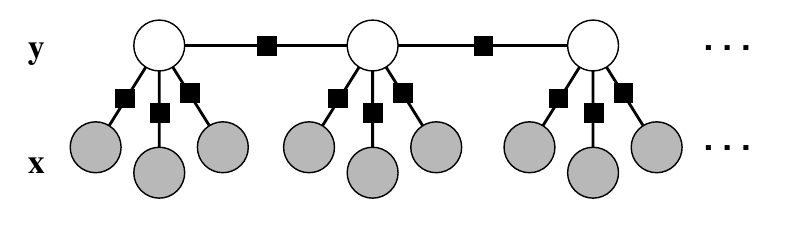
\includegraphics[scale = 0.4]{linear_chain_crf.png}
		\caption{Grafički model linearno ulančanog uvjetnog slučajnog polja}
	\end{figure}

%%%%%
% Singer: Popravio referencu - nije jednadzba, nego Definicija.
%%%%%
	S druge strane, distribucije nad proizvoljnim faktor grafovima, koje smo definirali u Definiciji \ref{factor_graph}, čine opća uvjetna slučajna polja.

	\begin{defn}
		Neka je $G = (V, F, E)$ faktor graf. Distribucija $\mathbb{P}(\mathbf{y} | \mathbf{x})$ je \tb{uvjet\-no slučajno polje} ako se faktorizira prema faktor grafu $G$ za svaki $\mathbf{x}$.
	\end{defn}

%%%%%
% Singer: Promijenio "nad" $G$ -> "iz" $G$.
%%%%%
	Drugim riječima, za skup faktora $F = \{ \Psi_A \}$ iz $G$, definiranih s
	\begin{equation*}
	\Psi_A(\mathbf{y}_A, \mathbf{x}_A) = \exp {\bigg\{\sum_{k} \theta_{Ak} f_{Ak} (\mathbf{y}_A, \mathbf{x}_A)\bigg\}},
	\end{equation*}
	se uvjetno slučajno polje zapisuje kao
	\begin{equation*}
	\mathbb{P}(\mathbf{y} | \mathbf{x})  = \frac{1}{Z(\mathbf{x})} \prod_{\Psi_A \in G} \exp \bigg(\sum_{k=1}^{|A|}  \theta_{Ak} f_{Ak} (\mathbf{y}_A, \mathbf{x}_A)\bigg).
	\end{equation*}

	U sljedećem dijagramu je jasan međusobni odnos naivnog Bayesovog klasifikatora, logističke regresije, skrivenih Markovljevih modela, te linearno ulančanih i općenitih uvjetnih slučajnih polja:

	\begin{figure}[H]
		\centering
		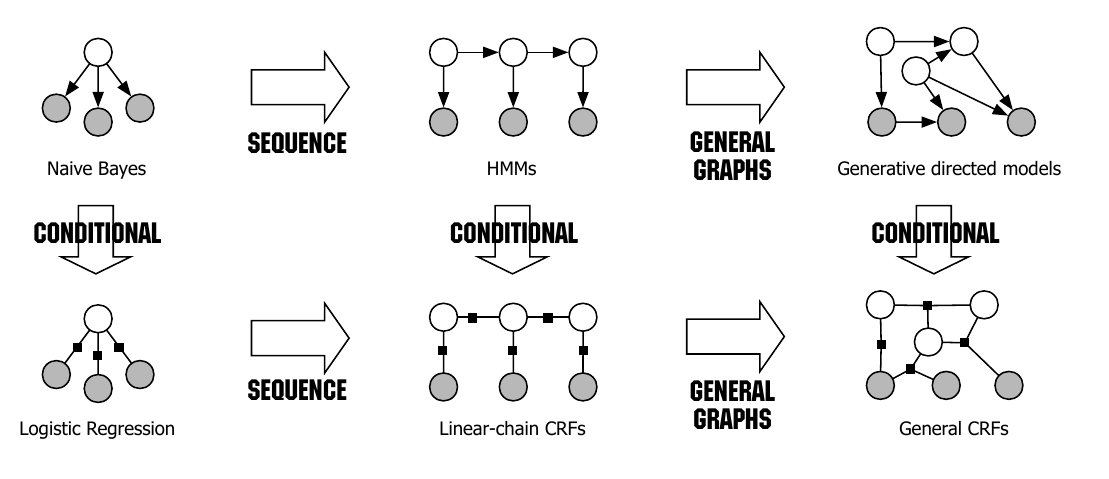
\includegraphics[scale = 0.50]{all_ner.png}
		\caption{Dijagram veza dosad navedenih modela}
	\end{figure}

	S obzirom da uvjetna slučajna polja u obzir uzimaju "širu sliku" nego skriveni Markovljevi modeli, imaju i šire područje primjene. Uz obradu prirodnog jezika, uvjetna slučajna polja uspješno rješavaju mnoge probleme računalnog vida, kao što je prepoznavanje objekata na slikama. Također, ovim modelom se postižu daleko najbolji rezultati u prepoznavanju imenovanih entiteta. \ti{Stanford NER}, jedan od najuspješnijih sustava, se temelji upravo na uvjetnim slučajnim poljima. Stanfordov sustav se sastoji od tri modela za engleski jezik, po dva za njemački i kineski, te jednog za španjolski jezik. Modeli za engleski jezik, ovisno o tome nad kojim skupom podataka su trenirani, prepoznaju:
	\begin{itemize}
		\item 	tri klase: \ti{Location}, \ti{Person}, \ti{Organization},
		\item	četiri klase: \ti{Location}, \ti{Person}, \ti{Organization}, \ti{Misc},
		\item 	sedam klasa: \ti{Location}, \ti{Person}, \ti{Organization}, \ti{Money}, \ti{Percent}, \ti{Date}, \ti{Time}.
	\end{itemize}

	\section{Učenje i korištenje modela}

	Za kraj ćemo opisati postupak određivanja, odnosno, učenja modela koji će se koristiti za prepoznavanje imenovanih entiteta.

	Neka je dan skup podataka za učenje $D = \{ (\mathbf{x}^{(1)}, \mathbf{y}^{(1)}), \ldots, (\mathbf{x}^{(N)}, \mathbf{y}^{(N)})\}$. Pretpostavljamo da su elementi skupa $D$ nezavisni i jednako distribuirani. Za svaki $i$ je $\mathbf{x}^{(i)} = \{x_1^{(i)}, \ldots, x_T^{(i)}\}$ $T$-dimenzionalni ulazni vektor, odnosno, niz riječi. S druge strane, $\mathbf{y}^{(i)} = \{y_1^{(i)}, \ldots, y_T^{(i)}\}$ je $T$-dimenzionalni vektor željenih izlaza. Željeni izlazi su, u ovom slučaju, točne oznake klasa niza riječi $\mathbf{x}^{(i)}$. Cilj je odrediti skriveni Markovljev model \eqref{hmm} ili linearno ulančani CRF \eqref{linear_crf}, koji će nad novim podacima što manje griješiti, odnosno, što točnije određivati klase.

	Učenje modela se sastoji u određivanju nepoznatih parametara ciljne funkcije za koje se postiže (po mogućnosti) globalni ekstrem. U ovom slučaju, nepoznati parametri su elementi vektora $\bm{\theta} = \{\theta_1, \ldots, \theta_K\}$.

	U slučaju skrivenih Markovljevih modela, za $\mathbb{P}(\mathbf{y}^{(i)}, \mathbf{x}^{(i)})$ kao u \eqref{hmm}, promatramo jednadžbu
	\begin{equation*}
	l(\bm{\theta}) = l(\theta_1, \ldots, \theta_K) = \sum_{i=1}^{N} \log \mathbb{P}(\mathbf{y}^{(i)}, \mathbf{x}^{(i)}).
	\end{equation*}

	Analogno, u slučaju linearno ulančanih uvjetnih slučajnih polja, za  $\mathbb{P}(\mathbf{y}^{(i)} | \mathbf{x}^{(i)})$ kao u \eqref{linear_crf}, imamo
	%%%%%
	% Singer: Dodao l(...) na samom pocetku.
	%%%%%
	\begin{equation*}
	l(\bm{\theta}) = l(\theta_1, \ldots, \theta_K) = \sum_{i=1}^{N} \log \mathbb{P}(\mathbf{y}^{(i)} | \mathbf{x}^{(i)}).
	\end{equation*}

	Postoji više metoda za određivanje maksimuma funkcije $l$ --- egzaktno, metodom gradijentog penjanja, ili nekom drugom heurističkom metodom. Metoda koja će se koristiti ovisi o veličini skupa za učenje i broju nepoznatih parametara, odnosno, složenosti funkcija značajki. U praksi se koriste veoma veliki skupovi za učenje, čija veličina se mjeri u stotinama tisuća riječi, te prilično složene funkcije značajki. Stoga se treniranje modela vrši na snažnim računalima uz brojne optimizacije. Unatoč tome, postupak može trajati satima.

	\bigskip

	Nakon određivanja parametara, možemo koristiti model za određivanje klase niza riječi, odnosno, prepoznavanje imenovanih entiteta u tekstu. Za zadani niz riječi $x$, računa se svaka od vjerojatnosti $\mathbb{P}(\mathbf{y}^{(k)} | \mathbf{x})$, pri čemu $\mathbf{y}^{(k)}$ predstavlja jedan mogući raspored dodijeljenih klasa, na primjer, $y_1 = \ti{Osoba}$, $y_2 = \ti{Osoba}$, $y_3 = \ti{Ostalo}$. I u ovom koraku problem može biti visoka složenost postupka, odnosno, dugotrajno izračunavanje. Naime, za niz riječi proizvoljne duljine $n$ i konstantan broj klasa $m$, potrebno je izračunati $m^n$ različitih vjerojatnosti, odnosno, postupak je eksponencijalne složenosti. Stoga su i za ovaj korak razvijene brojne optimizacije.


	\chapter{Modeli za razrješavanje koreferencije}

	\markboth{3. \ MODELI ZA RAZRJEŠAVANJE KOREFERENCIJE}{}

	\section{Model parova}

	U ovom poglavlju ćemo opisati nekoliko modela koji se koriste za razrješavanje koreferencije u tekstu, te navesti njihove prednosti i nedostatke. Započet ćemo s najjednostavnijim modelom, a to je \tb{model parova} (eng.~\ti{pairwise model}). Ovaj model razrješavanju koreferencije pristupa kao problemu binarne klasifikacije parova izraza. Definirajmo takav model.

	\begin{defn}
		Neka je za par izraza (slučajnih varijabli) $x_{ij} = \{x_i, x_j\}$ varijabla $y_{ij}$ definirana s
		\begin{equation*}
		y_{ij} = 1 \iff x_i \text{ i } x_j \text{ su koreferentni}.
		\end{equation*}
		Nadalje, neka je $F = \{f_k(x_{ij}, y_{ij})\}$ skup funkcija značajki nad $x_{ij}$, te neka su $\theta_k \in \mathbb{R}$ parametri. \tb{Model parova} se definira kao distribucija vjerojatnosti oblika
		\begin{equation}\label{pairwise}
		\mathbb{P} (y_{ij} | x_{ij}) =
		\frac {1}{Z_{x_{ij}}} \exp\bigg(\sum\limits_{k} \theta_k f_k(x_{ij}, y_{ij})\bigg),
		\end{equation}
		pri čemu je $Z_{x_{ij}}$ faktor normalizacije.
	\end{defn}

	Na primjer, funkcija $f_k(x_{ij}, y_{ij})$ može označavati jesu li $x_i$ i $x_j$ istog roda, dok funkcija $f_l(x_{ij}, y_{ij})$ označava jesu li jednake brojnosti.

	Ukoliko par $\{x_i, x_j\}$ smatramo uređenim parom, pri čemu izraz $x_i$ u tekstu prethodi izrazu $x_j$, te se $x_j$ odnosi na $x_i$, dobivamo asimetričnu interpretaciju problema razrješavanja koreferencije. Takva interpretacija je slična razrješavanju anafore. Jedina razlika je u tome što, kod anafore, izraz $x_j$ mora biti zamjenica koja se referira na izraz $x_i$. U ovom slučaju, $x_i$ i $x_j$ mogu biti bilo kakvi izrazi. Pogledajmo primjer:

	\bigskip

	\ti{$\underbracket{\text{Red Riding Hood}}_{x_{i}}$ was so happy. $\underbracket{\text{Young girl}}_{x_j}$ wanted to dance in the forest.}

	\bigskip

	Simetričnu interpretaciju dobivamo kada par $\{x_i, x_j\}$ interpretiramo kao ne\-ure\-đe\-ni par, pri čemu su $x_i$ i $x_j$ u koreferenciji, ali nije definiran smjer koreferencije.

	\bigskip

	Prednost modela parova je što je $\mathbb{P} (y_{ij} | x_{ij})$  moguće izračunati isključivo iz danog teksta, odnosno, pomoću parova $\{x_i, x_j\}$. S druge strane, model implicira pretpostavku o snažnoj neovisnosti među parovima. Rezultat toga je nemogućnost reprezentacije čitavog skupa izraza koji se odnose na isti entitet. Drugim riječima, dobivamo isključivo skupove oblika $\{ \ti{izraz}_i, \ti{izraz}_j\}$, a ne možemo dobiti skup izraza $\{ \ti{izraz}_1, \ldots, \ti{izraz}_n\}$ koji se referiraju na isti entitet.

	\bigskip

	Slično kao i u prethodnom poglavlju, modele za razrješavanje koreferencije možemo prikazati grafički i to na više načina.

	Prvi način prikaza je prilično intuitivan. U slučaju modela parova, kreiramo graf čiji vrhovi predstavljaju imeničke fraze, dok težine bridova odgovaraju vrijednostima $\mathbb{P}(y_{ij} | x_{ij})$. Sada se problem razrješavanja koreferencije svodi na particioniranje grafa u klastere s maksimalnim težinama bridova unutar pojedinog klastera te minimalnim težinama među klasterima. Jasnije je iz sljedeće slike:

	\vspace*{-6pt}
	\begin{figure}[H]
		\centering
		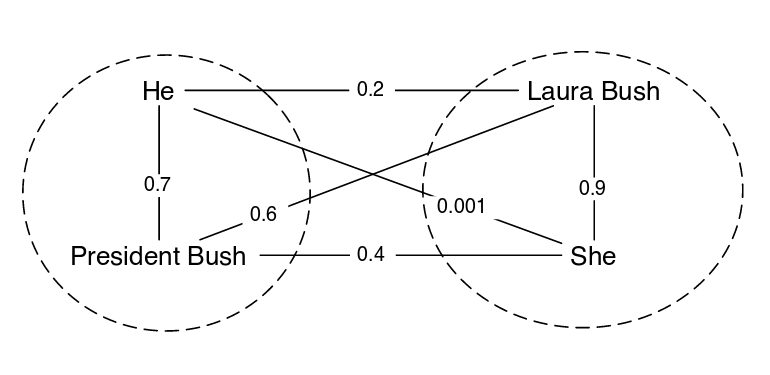
\includegraphics[scale = 0.5]{coreference_example.png}
		\caption{Primjer klasteriranja grafa}
	\end{figure}

	Drugi način koristi faktor grafove koje smo definirali u prethodnom poglavlju. Model za razrješavanje koreferencije prikazuje se faktor grafom. U takvom prikazu je jednostavno model parova proširiti tranzitivnošću izraza, čime dobivamo mogućnost reprezentiranja skupova izraza.

	Tranzitivnost izraza znači sljedeće: ako su $\ti{izraz}_1$ i $\ti{izraz}_2$, te $\ti{izraz}_2$ i $\ti{izraz}_3$ koreferentni, onda su $\ti{izraz}_1$ i $\ti{izraz}_3$, također, koreferentni. Na sljedećoj slici prikazan je primjer faktor grafa za model parova koji uključuje tranzitivnost.

	\begin{figure}[H]
		\centering
		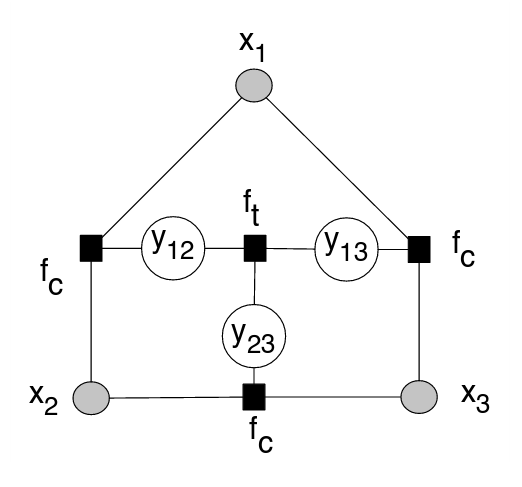
\includegraphics[scale = 0.5]{pairwise_factor_graph.png}
		\caption{Grafički prikaz modela parova}
	\end{figure}

	Faktori $f_c$ modeliraju koreferenciju dvaju izraza, dok faktor $f_t$ modelira tranzitivnost među izrazima. Sada možemo definirati grafički model parova za razrješavanje koreferencije.

	\begin{defn}
		\tb{Grafički model parova} za razrješavanje koreferencije čini distribucija uvjetne vjerojatnosti koja se faktorizira kao
		\begin{equation}\label{pairwise_graph}
		\mathbb{P}(\mathbf{y}| \mathbf{x}) =
		\frac{1}{Z_\mathbf{x}}
		\prod_{y_{ij} \in \mathbf{y}} f_c(y_{ij}, x_{ij})
		\prod_{y_{ij}, y_{jk} \in \mathbf{y}} f_t(y_{ij}, y_{jk}, y_{ik}, x_{ij}, x_{jk}, x_{ik}),
		\end{equation}
		pri čemu je ${Z_\mathbf{x}}$ normalizacijski faktor, faktor $f_c$ je definiran s
		\begin{equation*}
		f_c(y_{ij}, x_{ij}) = \exp\bigg(\sum\limits_{k} \theta_k f_k(y_{ij}, x_{ij})\bigg),
		\end{equation*}
		dok je faktor $f_t$ definiran s
		\begin{equation*}
		f_t(\cdot) =
		\begin{cases}
		-\infty, 		& \text{ako je tranzitivnost zadovoljena}, \\
		1,              & \text{inače}.
		\end{cases}
		\end{equation*}
	\end{defn}

	\bigskip

	Model parova se određuje analogno postupku opisanom na kraju prethodnog poglavlja. Neka je zadan skup nezavisnih jednako distribuiranih podataka $D = \{(x_{ij}, y_{ij})\}$, pri čemu par izraza $\{x_i, x_j\}$ može, ali i ne mora biti koreferentan. Cilj je nad zadanim podacima maksimizirati funkciju
	\begin{equation*}
	l(\bm{\theta}) = l(\theta_1, \ldots, \theta_K) = \sum_{ij} \log \mathbb{P}(y_{ij} | x_{ij}),
	\end{equation*}
	pri čemu je $\mathbb{P}(y_{ij} | x_{ij})$ kao u \eqref{pairwise} ili \eqref{pairwise_graph}.

	\bigskip

	Model se koristi na sljedeći način. Neka je zadan parametar $\delta \in \lbrack 0, 1\rbrack$ kojeg nazivamo prag vrijednosti. Izračunati model, za svaki par $\{x_i, x_j\}$ takav da je $\mathbb{P} (y_{ij} | x_{ij}) \geq \delta$, zaključuje da je međusobno koreferentan. Uobičajeni izbor za prag $\delta$ je 0.5. Što je prag veći, to će model biti precizniji. \tb{Preciznost} (eng.~\ti{precision}) se definira kao udio točno klasificiranih primjera u skupu pozitivno klasificiranih primjera. U ovom slučaju, visoka preciznost znači da su gotovo svi izrazi koje je model označio koreferentnima uistinu koreferentni. Uz preciznost, bitno svojstvo klasifikatora je i odziv. \tb{Odziv} (eng.~\ti{recall}) se definira kao udio točno klasificiranih primjera u skupu svih pozitivnih primjera. U ovom slučaju, brojni koreferentni izrazi neće biti označeni pa će odziv modela biti nizak.

	Obratno, za manji prag $\delta$, model će veći broj parova označiti kao koreferentne te će vjerojatno označiti većinu doista koreferentnih izraza. Dakle, model će imati visok odziv. S druge strane, vjerojatno će i dosta parova krivo označiti, pa će preciznost biti niska.

	Dakle, za uspješno razrješavanje koreferencije potrebno je da model ima što više i preciznosti i odziva. Te dvije mjere se objedinjuju u jednu mjeru kvalitete koju nazivamo $F$-mjera.

	\begin{defn}
		$\bm{F_\beta}$\tb{-mjera}, za $\beta \in \mathbb{R}$, se definira kao
		\begin{equation*}
		F_\beta = (1+\beta^2) \, \frac
		{\ti{preciznost} \cdot \ti{odziv}}
		{\beta^2 \cdot \ti{preciznost} + \ti{odziv}}.
		\end{equation*}
		Posebno, $\bm{F_1}$\tb{-mjera} se definira kao
		\begin{equation*}
		F_1 = 2 \cdot \frac
		{\ti{preciznost} \cdot \ti{odziv}}
		{\ti{preciznost} + \ti{odziv}}.
		\end{equation*}
	\end{defn}

	$F$-mjera poprima vrijednosti između $0$ i $1$, pri čemu je model kvalitetniji što je njegova $F$-mjera viša.

	Parametar $\beta$ određuje kojem svojstvu pridajemo veću važnost, preciznosti ili odzivu. Na primjer, za $\beta = 0.5$ dvostruko veću važnost pridajemo preciznosti nego odzivu, dok je za $\beta = 2$ obratno. Najčešće se koristi $F_1$-mjera koja za obje stavke pridjeljuje jednaku važnost.

	\section{Model logike prvog reda}

	\tb{Model logike prvog reda} (eng.~\ti{First-order logic model}) za razrješavanje koreferencije se razvio s ciljem rješavanja problema reprezentacije skupa izraza. Model je analogan prethodno opisanom modelu.

	\begin{defn}
		Neka je $\mathbf{x}^j = \{x_i\}$ skup imeničkih fraza i neka je varijabla $y_j$ definirana s
		\begin{equation*}
		y_j = 1 \iff \text{sve fraze } x_i \in \mathbf{x}^j  \text{ su međusobno koreferentne}.
		\end{equation*}
		\tb{Model logike prvog reda} definiramo kao distribuciju vjerojatnosti oblika
		\begin{equation}\label{first_order}
		\mathbb{P} (y_{j} | \mathbf{x}^j) =
		\frac {1} {Z_{\mathbf{x}^j}} \exp \bigg(\sum\limits_{k} \theta_k f_k(\mathbf{x}^j, y)\bigg),
		\end{equation}
		pri čemu su $f_k$ funkcije značajke nad čitavim skupom $\mathbf{x}^j$, a $\theta_k \in \mathbb{R}$ su pripadni parametri.
	\end{defn}

	I ovaj model možemo prikazati pomoću faktor grafova, kao na sljedećoj slici:
	\begin{figure}[H]
		\centering
		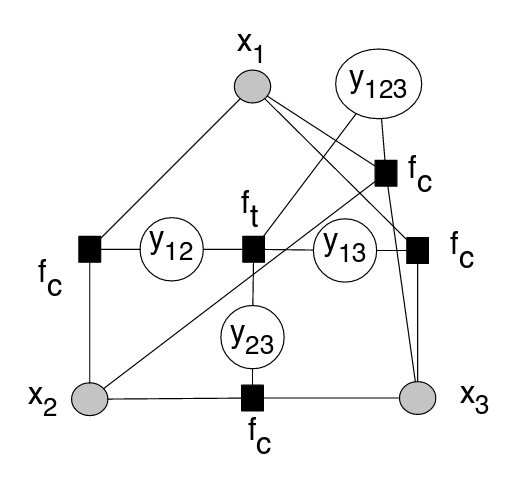
\includegraphics[scale = 0.5]{first_order_logic_factor_graph.png}
		\caption{Grafički prikaz modela logike prvog reda}
	\end{figure}

	Faktori $f_c$ i $f_t$ imaju jednaku ulogu kao i u modelu parova. Tranzitivnost je nešto kompliciranija: ako je $y_j = 1$, za svaki podskup $\mathbf{x}^k \subseteq \mathbf{x}^j$ mora vrijediti $y_k = 1$. Nadalje, uvodi se dodatni čvor $y_{I}$, pri čemu je $I$ neki skup indeksa, koji označava jesu li svi izrazi $\mathbf{x}^I$ međusobno koreferentni. Uočimo da broj čvorova $y_I$ raste eksponencijalno u odnosu na broj ulaznih varijabli $x$.

	\begin{defn}
		\tb{Grafički model logike prvog reda} za razrješavanje koreferencije čini distribucija uvjetne vjerojatnosti koja se faktorizira kao
		\begin{equation}\label{first_order_logic_graph}
		\mathbb{P}(\mathbf{y}| \mathbf{x}) =
		\frac{1}{Z_\mathbf{x}}
		\prod_{y_{j} \in \mathbf{y}} f_c(y_j, \mathbf{x}^j)
		\prod_{y_{j} \in \mathbf{y}} f_t(y_j, \mathbf{x}^j),
		\end{equation}
		pri čemu je ${Z_\mathbf{x}}$ normalizacijski faktor, faktor $f_c$ je definiran s
		\begin{equation*}
		f_c(y_j, \mathbf{x}^j) = \exp\bigg(\sum\limits_{k} \theta_k f_k(y_{j}, \mathbf{x}^j)\bigg),
		\end{equation*}
		dok je faktor $f_t$ definiran s
		\begin{equation*}
		f_t(\cdot) =
		\begin{cases}
		-\infty, 		& \text{ako je tranzitivnost zadovoljena}, \\
		1,              & \text{inače}.
		\end{cases}
		\end{equation*}
	\end{defn}

	\bigskip

	Posebnog ovog modela je u tome što, ako je potrebno, skup podataka za treniranje možemo jednostavno proširiti. Pozitivne (međusobno koreferentne) skupove $\mathbf{x}^j$ generiramo slučajnim, uniformnim uzorkovanjem nekog pozitivnog skupa $\mathbf{x}^k$, nakon čega uzorkujemo podskup tog skupa. S druge strane, negativne skupove dobivamo uzorkovanjem dva različita pozitivna skupa i spajanjem u jedan skup. Na primjer, neka su zadani koreferentni skupovi \{\ti{Red Riding Hood}, \ti{young girl}, \ti{granddaughter}, \ti{child}\} te \{\ti{evil wolf}, \ti{beast}\}. Pozitivan skup je bilo koji podskup prvog skupa, poput \{\ti{granddaughter}, \ti{child}\}. S druge strane, negativan skup je \{\ti{Red Riding Hood}, \ti{evil wolf}\}.

	\bigskip

	Učenje modela logike prvog reda je analogno učenju modela parova. Jedina razlika je u obliku podataka za učenje i ciljne funkcije $l(\bm{\theta})$, koja je sad oblika
	\begin{equation*}
	l(\bm{\theta}) = l(\theta_1, \ldots, \theta_K) = \sum_{ij} \log \mathbb{P} (y_{j} | \mathbf{x}^j),
	\end{equation*}
	pri čemu je $\mathbb{P}(y_{ij} | \mathbf{x}^j)$ kao u \eqref{first_order} ili \eqref{first_order_logic_graph}.

	\bigskip

	Model se primjenjuje u tekstu na sljedeći način. Nad imeničkim frazama se prvo odvija pohlepno aglomerativno klasteriranje, odnosno, nenadzirano grupiranje imeničkih fraza. Svako grupiranje ocjenjujemo proporcionalno vjerojatnosti takvog skupa u modelu. Postupak završava kada više ne postoji grupiranje koje bi povećalo ocjenu dobivenog skupa, odnosno, vjerojatnost da su svi elementi tog klastera međusobno koreferentni. Na primjer, neka se u tekstu fraze \ti{Red Riding Hood}, \ti{young girl}, \ti{child}, \ti{granddaughter}, \ti{she} odnose na Crvenkapicu. Uz njih, algoritam je pronašao i fraze \ti{evil wolf}, \ti{old lady}. Postupak može izgledati ovako:

	\begin{enumerate}[label=\tb{\arabic*:}, align=left, labelwidth=13pt]
		\item	Grupiraju se \{\ti{Red Riding hood}, \ti{young girl}\}. Vjerojatnost dobivenog skupa je $0.64$.
		\item	Grupiraju \{\ti{Red Riding hood}, \ti{young girl}, \ti{child}\}. Vjerojatnost dobivenog skupa iznosi $0.7$.
		\item	Ne grupiraju se \{\ti{Red Riding hood}, \ti{young girl}, \ti{child}\} i \{\ti{old lady}\}, jer bi vjerojatnost tako dobivenog skupa bila $0.2$.
		\item	Grupiraju se  \{\ti{granddaughter}\} i  \{\ti{she}\}. Vjerojatnost dobivenog skupa je $0.4$.
		\item	Grupira se \{\ti{Red Riding hood}, \ti{young girl}, \ti{child}\} i \{\ti{granddaughter}, \ti{she}\} u jedan skup vjerojatnosti $0.8$.
		\item	Ne grupira se \{\ti{Red Riding hood}, \ti{young girl}, \ti{child}, \ti{granddaughter}, \ti{she}\} i \{\ti{evil wolf}\}, jer bi vjerojatnost tako dobivenog skupa bila $0.1$.
		\item	Postupak završava, jer su svi izrazi obuhvaćeni.
	\end{enumerate}


	\section{Metoda višeprolaznog sita}

	\tb{Metoda višeprolaznog sita} (eng.~\ti{multi-pass sieve}) je modularna metoda koju koristi Stanford Deterministic Coreference Resolution System, jedan od danas najuspješnijih i najpoznatijih sustava za razrješavanje koreferencije.

	Većina pristupa rješavanju problema koreferencije se temelji na korištenju jedinstvene funkcije nad skupom ograničenja, odnosno, svojstava. Promatraju se lokalna leksička, sintaktička, semantička i/ili diskurzivna svojstva teksta. To nipošto nije loše --- ovakav pristup je rezultirao veoma kvalitetnim rješenjima~\cite{haghighi2009simple}. Unatoč tome, u praksi se javljaju određeni problemi.

	Prvi problem ovog pristupa se javlja zbog prevelikog broja svojstava. Neka svojstva se u tekstu mogu javljati veoma često, ali sama po sebi nisu jako precizna. S druge strane, postoje i svojstva koja se javljaju rijetko, ali su vrlo precizna. Kako funkcija uzima u obzir sva svojstva, postoji mogućnost da u izračunu prevagnu češća, manje precizna svojstva, odnosno, da se zanemare one karakteristike koje daju točno rješenje. Drugi problem je u lokalnosti informacija. Često ne možemo iz neposredne okoline ispravno zaključiti s kojim entitetom je izraz u koreferenciji, već treba promatrati širu okolinu izraza.

	Metoda višeprolaznog sita primjenjuje modele, počevši od najpreciznijeg, prema najmanje preciznome. Svaki model gradi nad prethodno dobivenim informacijama --- u svakom se koraku koriste sve dotad poznate informacije. Metoda koristi isključivo determinističke modele, odnosno, pri svakoj primjeni neke komponente dobiva se jednak rezultat. Svaka od komponenti je oblikovana nenadziranim učenjem. To znači da nije potrebno imati velike skupove ručno označenih podataka za učenje do kojih je, kao što smo ranije spomenuli, mukotrpno doći, već je dovoljno predati podatke modelu i on će ih automatski obraditi.

	\bigskip

	\tb{Stanford Deterministic Coreference Resolution System} se sastoji primarno od dvije faze, otkrivanja navoda (eng.~\ti{mentions}) i razrješavanja koreferencije.
	Na slici \ref{sieve} vidimo građu ovog sustava.

	\begin{figure}[H]
		\centering
		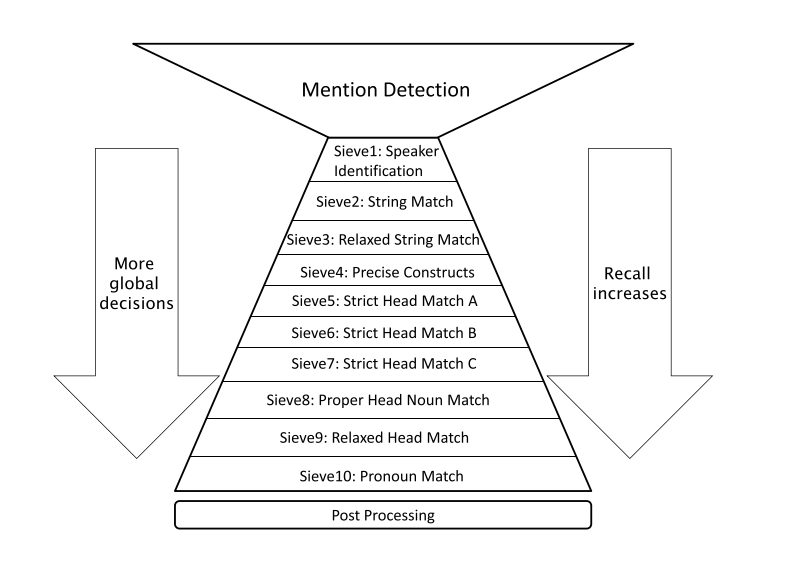
\includegraphics[scale = 0.71]{sieve.png}
		\caption{Građa Stanfordovog sustava za razrješavanje koreferencije}
		\label{sieve}
	\end{figure}

	U prvoj fazi se algoritmom visokog odziva otkrivaju svi navodi --- imeničke fraze, zamjenice, imenovani entiteti. Visoki odziv znači da su u tekstu označeni gotovo svi navodi entiteta. Potom se iz tog skupa izbacuju svi izrazi koji nisu navodi, poput numeričkih entiteta, pleonastičkog \ti{it}\footnote{Primjer pleonastičkog \ti{it} je rečenica \ti{"\tb{It} rains."}. U hrvatskom jeziku su analogon besubjektne rečenice, poput \ti{Kiši.}}, ili partitiva\footnote{Partitivi određuju količinu nebrojivih imenica, poput \ti{\tb{half} of cookies}, \ti{\tb{bag} of flour}. U hrvatskom jeziku je takva struktura poznata pod nazivom dijelni genitiv.}.

	U drugoj fazi se nad označenim tekstom primjenjuje deset nezavisnih modela za razrješavanje koreferencije. Svi modeli su testirani nad istim, unaprijed određenim skupom podataka, čime se utvrđuje njihova preciznost. Prednost nezavisnih modela je ta što, u bilo kojem trenutku, na bilo kojoj razini, možemo nadograditi sustav novim modelima. Ti modeli koriste sve informacije koje su dotad poznate sustavu --- na primjer, u zadnjem koraku, razrješavanju zamjeničke koreferencije, osim okoline navoda, koristimo podatke kao što su vrsta entiteta, spol, broj (jednina/množina) i lema\footnote{Rječnička natuknica ili lema je osnovna riječ u rječniku, leksikonu ili enciklopediji, koja se objašnjava, odnosno, definira i s kojom započinje članak takve knjige.}.

	Upravo iz dvofazne arhitekture slijedi visoka preciznost i visok odziv sustava, odnosno, visoka $F$-mjera sustava. Konkretno, prema~\cite{lee2013deterministic}, prosječna $F$-mjera dobivena testiranjem nad više velikih skupova podataka iznosi $0.5956$. To se naizgled ne čini mnogo, ali je vrlo dobar rezultat kad se u obzir uzme složenost problema.

	\chapter{Modeli za analizu sentimenta}

	\markboth{4. \ MODELI ZA ANALIZU SENTIMENTA}{}

	\section{Model "vreća riječi"}

	Model \tb{"vreća riječi"} (eng.~\ti{bag-of-words model}) je najjednostavniji model koji se koristi u analizi sentimenta. Model se, također, može koristiti i za otkrivanje spam e-mailova. Tekst se prikazuje isključivo kao skup riječi koje ga čine. Preciznije, model promatra multiskup riječi, s obzirom da je važno koliko često se javlja pojedina riječ, ali se ignorira njihov poredak. Također je moguće ignorirati i oblik riječi, odnosno, promatrati isključivo infinitive glagola, jednine imenica i slično.

	Na primjer, rečenicu \ti{"This story is interesting and it has good characters and good ending."} možemo prikazati sljedećom "vrećom riječi":

	\begin{center}
		\begin{tabular}{lc}
			Riječ                & \multicolumn{1}{l}{Frekvencija} \\ \hline
			\ti{this}        & 1                               \\
			\ti{story}       & 1                               \\
			\ti{is}          & 1                               \\
			\ti{interesting} & 1                               \\
			\ti{and}         & 2                               \\
			\ti{it}          & 1                               \\
			\ti{has}         & 1                               \\
			\ti{good}        & 2                               \\
			\ti{characters}  & 1                               \\
			\ti{ending}      & 1
		\end{tabular}
	\end{center}

	Za određivanje sentimenta rečenice je dovoljno odrediti koliko ima pozitivnih riječi, a koliko negativnih. Ako ima više pozitivnih riječi nego negativnih, sentiment je pozitivan. U protivnom je negativan.

	Preduvjet tom koraku je oblikovanje skupova svih pozitivnih i svih negativnih riječi. Takvi skupovi su obično dostupni na internetu, te su sortirani abecedno:
	\begin{displayquote}
		\ti{Positive} = \{\ti{acclaim}, \ldots, \ti{blessing}, \ldots, \ti{captivate}, \ldots, \ti{divine}, \ldots \},\\[3pt]
		\ti{Negative} = \{\ti{absurd}, \ldots, \ti{betrayal}, \ldots, \ti{cheating}, \ldots, \ti{death}, \ldots \}.
	\end{displayquote}

	Za svaku riječ u vreći provjeravamo nalazi li se u nekom od ova dva skupa i, ovisno o tome, ju bodujemo pozitivno ili negativno, s onoliko bodova kolika je frekvencija te riječi. U gornjem primjeru imamo dvije pozitivne riječi, \ti{interesting} i \ti{good}, koje se ukupno javljaju tri puta. Kako nemamo nijednu negativnu riječ, konačno stanje bodova je 3, te zaključujemo da je rečenica pozitivnog stava.

	S obzirom da metoda ignorira poredak riječi, gramatiku i bilo kakve dodatne informacije koje možemo izvući iz teksta, česte su pogreške. Na primjer, metoda jednako promatra sljedeće izjave:
	\begin{displayquote}
		\ti{I am disappointed. This book is not very good.}\\
		\ti{I am not disappointed. This book is good.}
	\end{displayquote}
	U oba slučaja rezultat će biti neutralan stav. Naime, po jednom se javljaju pozitivna riječ \ti{good} i negativna riječ \ti{disappointed}. Ostale riječi nisu prepoznate kao pozitivne ili negativne.

	Ovaj problem možemo riješiti tako da, osim samih riječi, odnosno, unigrama, promatramo i bigrame ili trigrame. Na primjer, ukoliko se u rečenici javlja neka od riječi \ti{not}, \ti{just}, \ti{very}, \ti{no}, nju i njezinog sljedbenika promatramo kao cjelinu, dok sljedbenika više ne promatramo zasebno. Na primjer, izraz \ti{not good} se promatra kao negacija pozitivne riječi \ti{good}, pa zaključujemo da je izraz negativan. Samu riječ \ti{good} više ne uzimamo u obzir za bodovanje.

	\section{Model "vreća stavova"}

	Model \tb{"vreća stavova"} (eng.~\ti{bag-of-opinions}) je nastao kao odgovor na probleme modela "vreće riječi". Model, također, omogućuje relativno uspješnu stupnjevitu analizu sentimenta, na primjer, raspoznavanje vrlo pozitivnih od umjereno pozitivnih stavova.

	Ovaj model promatra tekst kao skup stavova s proizvoljnim brojem modifikatora i negatora. Možemo ga opisati na sljedeći način.

	Neka se tekst $\mathbf{x}$ sastoji od skupa stavova $O = \{ \mathbf{o}_1, \ldots, \mathbf{o}_n \}$. Svaki stav $\mathbf{o}_i$ se sastoji od:
	\begin{itemize}
		\item	korijena $w_r$, za neki $r \in R$, pri čemu je $R$ skup svih indeksa korijena teksta~$\mathbf{x}$,
		\item 	skupa modifikatora $\{w_m \mid m \in M'\}$, pri čemu je $M'$ podskup skupa $M$ svih indeksa modifikatora teksta $\mathbf{x}$,
		\item 	skupa negatora $\{w_z \mid z \in Z'\}$, pri čemu je $Z'$ podskup skupa $Z$ svih indeksa negatora teksta $\mathbf{x}$.
	\end{itemize}

	Za proizvoljni stav $\mathbf{o}$ u tekstu, definiramo funkciju $\ti{score} : O \to \mathbb{R}$ na sljedeći način:
	\begin{equation*}
	\ti{score} (\mathbf{o}) = \text{ sign} (r) \beta_r x_r
	+ \sum_{m \in M}\text{sign}(r) \beta_m x_m
	+ \sum_{z \in Z}\text{sign}(r) \beta_z x_z.
	\end{equation*}

	Funkcija $\text{sign} : R \to \{-1, 1\}$ označava polaritet stava i definira se kao
	\begin{equation*}
	\text{sign}(r) =
	\begin{cases}
	1, 	& \text{korijen } w_r \text{ je pozitivan}, \\
	-1,     & \text{korijen } w_r \text{ je negativan}.
	\end{cases}
	\end{equation*}

	Nadalje, $\beta_i$ su težine svakog elementa stava $\mathbf{o}$. Na primjer, \ti{extremely} ima značajno veću težinu od \ti{slightly}. Iz samog modela slijedi da težine modifikatora moraju biti pozitivne, dok su negatori negativnih težina, s obzirom da mijenjaju stav u suprotan.

	Također, $x_z$, $x_m$, $x_r$ su binarne varijable definirane s
	\begin{equation*}
	x_i =
	\begin{cases}
	1, 	& w_i \text{ je prisutan u stavu } \mathbf{o}, \\
	0,      & \text{inače}.
	\end{cases}
	\end{equation*}

	Konačno, funkcija $f$, koja za tekst $\mathbf{x}$ predviđa sentiment, definira se kao prosjek ocjena svih stavova pronađenih u tekstu:
	\begin{equation}
	f(\mathbf{x}) = \frac{1}{n} \sum_{i=1}^{n} \ti{score} (\mathbf{o}_i).
	\end{equation}

	Slično kao i u "vreći riječi", ako je $f(\mathbf{x}) \ge 0$, zaključujemo da je stav pozitivan. Ukoliko je $f(\mathbf{x}) \le 0$, stav je negativan. Dodatno, ovisno o vrijednosti $f(\mathbf{x})$, možemo stupnjevati stav --- stav je vrlo negativan, umjereno negativan, umjereno pozitivan, ili vrlo pozitivan.

	Parametri modela $\bm{\beta} = \{\beta_r, \beta_m, \beta_z \mid r \in R, m \in M, z \in Z \}$ se određuju učenjem nad označenim podacima, slično postupcima opisanim u prethodnom poglavlju. Ovdje je postupak nešto kompliciraniji pa ga nećemo detaljno opisivati. Također, nećemo opisivati postupak prepoznavanja stavova u tekstu, s obzirom da je to zaseban problem.

	\section{Naivni Bayesov klasifikator}

	U prethodnom poglavlju smo opisali naivni Bayesov klasifikator. Sada ćemo opisati kako se on može koristiti za analizu sentimenta.

	Naivni Bayesov klasifikator, također, možemo promatrati kao svojevrsno una\-prje\-đe\-nje modela "vreće riječi". Naime, prvi korak je izgraditi vreću riječi zadanog teksta, ali za određivanje sentimenta nećemo koristiti ranije opisani sustav "bodovanja", već sljedeći postupak.

	Neka je dan tekst $\mathbf{x}$, duljine $n$, u kojem su označene riječi koje opisuju pozitivan, odnosno, negativan sentiment. Neka je $c$ oznaka neke od klasa \ti{pozitivno}, \ti{negativno}. Za svaku riječ $w_i$ u tekstu računamo sljedeću vjerojatnost:
	\begin{equation*}
	\mathbb{P}(w_i | c) = \frac{\ti{count}(w_i, c) + 1}{\ti{count}(w, c) + n},
	\end{equation*}
	pri čemu $\ti{count}(w_i, c)$ označava broj pojava riječi $w_i$ koje su označene klasom $c$, dok $\ti{count}(w, c)$ označava ukupan broj riječi u tekstu označenih klasom $c$.

	Za čitavi tekst $\mathbf{x}$ potom računamo
	\begin{equation*}
	\mathbb{P}(\mathbf{x} | c) = \mathbb{P}(c) \prod_{i=1}^{n} \mathbb{P}(w_i | c),
	\end{equation*}
	pri čemu je $ \mathbb{P}(c)$ vjerojatnost pojedine klase.
	Konačno, zaključujemo da tekst pripada onoj klasi $c$ za koju gornji izraz postiže maksimum.

	\section{Duboko učenje}

	Za sam kraj, opisujemo jednu od danas najuspješnijih metoda analize sentimenta koja je razvijena na Sveučilištu u Stanfordu. Radi se o \tb{dubokom učenju} (eng.\ \ti{deep learning}), konkretno, o \tb{rekurzivnim dubokim modelima za se\-man\-ti\-čku djeljivost nad Sentiment Treebankom} (eng.~\ti{Recursive deep models for semantic compositionality over a Sentiment Treebank}).

	\bigskip

	Za početak, objasnimo uopće pojam dubokog učenja. \tb{Duboko učenje} je vrlo mlada grana strojnog učenja, čiji cilj je podatke reprezentirati vrlo složenim modelima, koji su rezultat niza nelinearnih transformacija. Jedan takav model se sastoji od više slojeva koji su, najčešće, oblikovani nenadziranim učenjem. Svaki sloj za ulaz uzima izlaz prethodnog sloja i možemo ga shvatiti kao jednu razinu apstrakcije podataka. Prvi sloj, najčešće, za cilj ima prepoznati bitne karakteristike ulaznih podataka (eng.~\ti{feature extraction}). Na primjer, ukoliko je modelu za prepoznavanje lica predana fotografija, prvi sloj može prepoznati određene točke na fotografiji (kutovi usana, očiju, krajevi obrva), dok neki kasniji sloj obrađuje isječke dane fotografije (usne, oči, obrve).

	Modeli dobiveni dubokim učenjem se uspješno primjenjuju za rješavanje problemima u kojima je složenost podataka veoma visoka, poput obrade prirodnog jezika ili računalnog vida.

	\bigskip

	Duboko učenje se pretežno temelji na neuronskim mrežama. \tb{Neuronske mre\-že} (eng.~\ti{neural networks}) su model strojnog učenja motiviran biološkim neuronima, odnosno, ljudskim mozgom. Biološki neuron se sastoji od tijela, ulaznih veza koje nazivamo dendriti i izlazne veze koju nazivamo akson. Ukoliko jačina ulaznih signala na dendritima prijeđe neku granicu, neuron se aktivira i šalje određenu vrijednost preko aksona. Sljedeći neuroni taj izlaz primaju kao svoj ulaz te se postupak ponavlja.

	Shodno tome, umjetnu neuronsku mrežu čini slojevito organiziran skup umjetnih neurona. Veze među neuronima u slojevima $k$ i $k + 1$ imaju težine $w_{ij}^{(k)}$, koje određuju utjecaj određenog ulaza (s neurona $i$ na sloju $k$) na rezultat neurona $j$ na sloju $k + 1$. Uobičajeno se u svakom sloju dodaje dodatni neuron koji određuje pristranost ili pomak (eng.~\ti{bias}) ulaza. Početni sloj neurona se naziva \tb{ulazni sloj} (eng.~\ti{input layer}) i prima vektor ulaznih podataka $\mathbf{x}$. Ulaz se prosljeđuje sljedećem sloju neurona. U svakom od tih neurona se računa vrijednost \tb{aktivacijske funkcije}. Ona može biti proizvoljnog oblika, ali najčešće se koristi sigmoidalna funkcija definirana s
	\begin{equation*}
	\psi(\mathbf{v}) = \frac{1}{1+e^{-\mathbf{v}}},
	\end{equation*}
	pri čemu je $\mathbf{v}$ težinska linearna kombinacija svih ulaza i pomaka, za odgovarajući neuron.

	Neuron, kao izlaz, šalje izračunatu vrijednost aktivacijske funkcije za svoj ulaz. Sljedeći sloj neurona prima te vrijednosti kao ulaz i ponavlja računanje. Postupak završava u zadnjem, \tb{izlaznom sloju} (eng.~\ti{output layer}). Svi slojevi neurona između ulaznog i izlaznog sloja se nazivaju \tb{skriveni slojevi} (eng.~\ti{hidden layers}).

	Uobičajeno se ulazni sloj ne uračunava u broj slojeva mreže, s obzirom da se u njemu ne odvija nikakvo računanje. Stoga, kad kažemo "jednoslojna mreža" mislimo na mrežu sastavljenu samo od ulaznog i izlaznog sloja.

	\bigskip

	Na sljedećoj slici prikazana je arhitektura jedne jednostavne neuronske mreže. S $L_1$ je označen ulazni sloj mreže. Slojevi $L_2$ i $L_3$ su skriveni slojevi, dok je $L_4$ izlazni sloj. Ulazni sloj $L_1$ prima zadani ulazni vektor $\mathbf{x} = (x_1, x_2, x_3)$. Na svakom sloju, s $+1$ su označeni dodatni neuroni koji generiraju pomak i time utječu na izlaz aktivacijske funkcije za zadani ulaz. Na slici su označene samo težine veza između prvih neurona na slojevima $k$ i $k + 1$, uz skraćenu oznaku $w_1^{(k)} = w_{11}^{(k)}$.

	\begin{figure}[H]
		\centering
		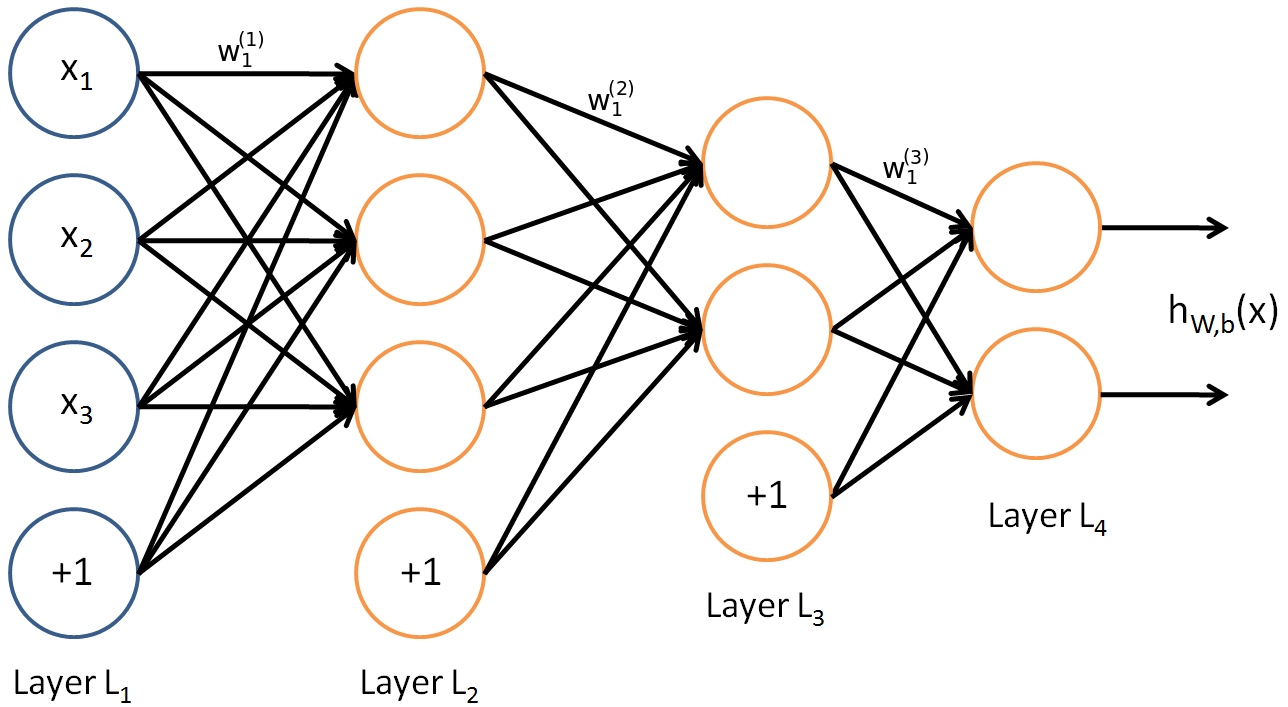
\includegraphics[scale = 0.35]{network.png}
		\caption{Primjer neuronske mreže}
	\end{figure}

	Neuronske mreže koje se koriste u dubokom učenju su vrlo kompleksne arhitekture. Konkretno, Stanfordov model za analizu sentimenta koristi \tb{rekurzivne neuronske tenzorske mreže} (eng.~\ti{recursive neural tensor networks}).

	Prvo opišimo općenite rekurzivne neuronske mreže. Ove mreže se koriste za određivanje strukture podataka i to pomoću stabala. Svaki čvor-roditelj u stablu se prikazuje kao nelinearna transformacija svojih čvorova-djece. Drugim riječima, svi čvorovi, osim listova, nastali su kao izlaz (iste) neuronske mreže, kojoj su kao ulaz dani čvorovi nastali u prethodnom koraku. Očito se radi o rekurzivnom postupku koji započinje s listovima, a završava s korijenom stabla.

	Rekurzivne neuronske mreže se najviše koriste u obradi prirodnog jezika i od\-re\-đi\-va\-nju strukture slika (primjer toga je prepoznavanje ceste, stabla i neba, kao zasebnih cjelina na slici).

	\bigskip

	Na sljedećem nizu slika vidimo primjer određivanja gramatičke strukture re\-če\-ni\-ce rekurzivnom neuronskom mrežom. Na početku je svaka riječ predstavljena nekim vektorom. Te riječi čine listove budućeg stabla. Neuronska mreža računa moguće roditelje tih listova u stablu. Osim vrijednosti vektora, izračunava se i njegova ocjena. Što je ta ocjena viša, to je vjerojatnije da je dobiveni čvor ispravan. Na slikama su zelenom bojom označene visoke ocjene čvorova. Takve čvorove zadržavamo u stablu. S druge strane, crvenom bojom su označene loše ocjene čvorova. Te čvorove odbacujemo.

	Za rečenicu \ti{"The cat sat on the mat."}, na slikama su prikazana prva $3$ koraka parsiranja i završno stablo parsiranja.

	\begin{figure}[H]
		\centering
		\vspace*{-20pt}
		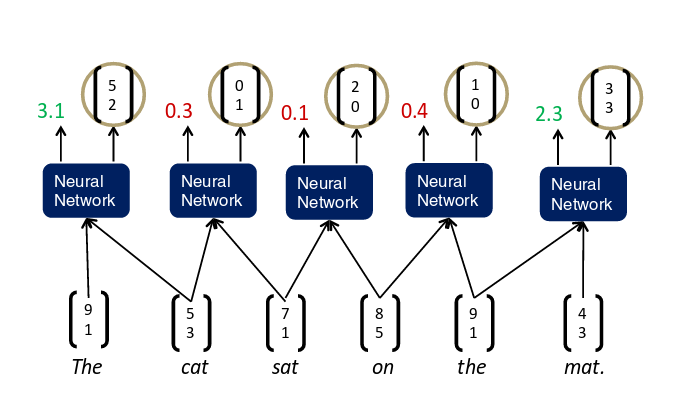
\includegraphics[scale = 0.70]{recursive_parse_1.png}

		\vspace*{-12pt}
		\caption{Prvi korak parsiranja --- "\underline{the cat}" i "\underline{the mat}" su dobri čvorovi pa ih zadržavamo.}
	\end{figure}

	\begin{figure}[H]
		\centering
		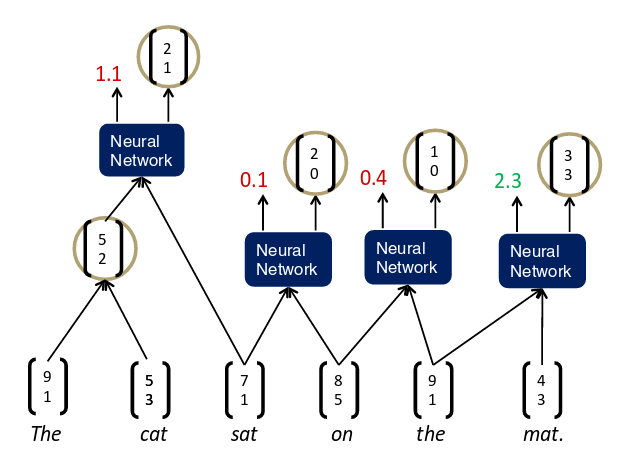
\includegraphics[scale = 0.70]{recursive_parse_2.png}

		\vspace*{-6pt}
		\caption{Drugi korak parsiranja --- svi novi čvorovi su loši te ih odbacujemo.}
	\end{figure}

	\newpage

	\begin{figure}[H]
		\centering
		\vspace*{-12pt}
		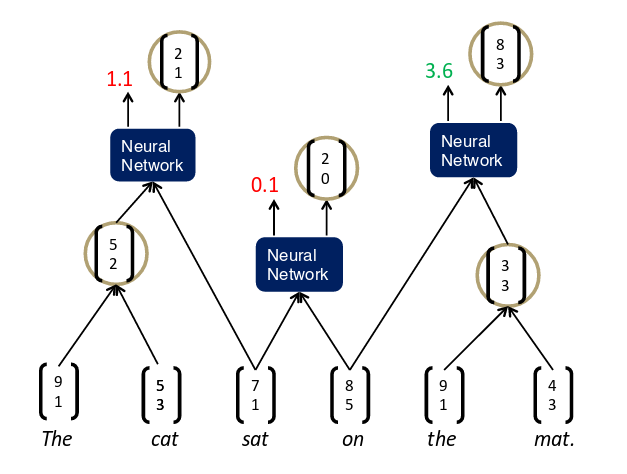
\includegraphics[scale = 0.70]{recursive_parse_3.png}

		\vspace*{-6pt}
		\caption{Treći korak parsiranja --- čvor "\underline{on} \underline{the mat}" je dobar te ga dodajemo u stablo.}
	\end{figure}

	\begin{figure}[H]
		\centering
		\vspace*{-24pt}
		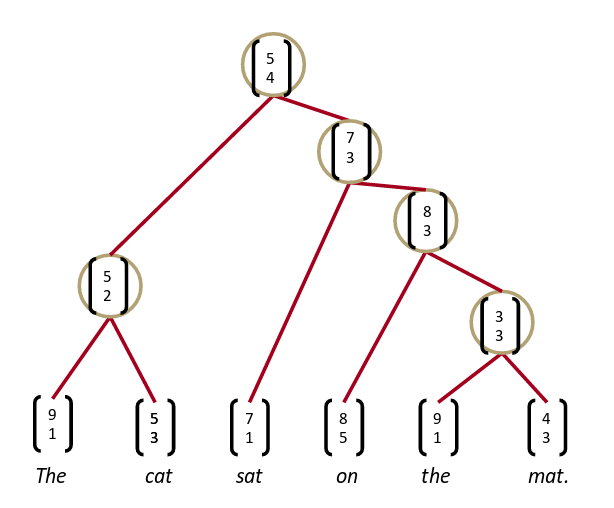
\includegraphics[scale = 0.70]{recursive_parse_4.png}

		\vspace*{-6pt}
		\caption{Završno stablo parsiranja --- s obzirom da je novi čvor korijen, postupak završava.}
	\end{figure}

	U osnovnim rekurzivnim neuronskim mrežama, vrijednost $d$-dimenzionalnog vektora čvora-roditelja se računa na sljedeći način. Neka su $l$, $r$ oznake za, redom, lijevo i desno dijete čvora $p$. Označimo s $h_p$ vrijednost vektora roditelja $p$. S $h_l$ i $h_r$ označimo, redom, vrijednosti vektora djece $l$ i $r$. Tada je
	\begin{equation*}
	h_p = f \bigg(
	W
	\begin{bmatrix}
	h_l \\
	h_r
	\end{bmatrix}
	+ b
	\bigg),
	\end{equation*}
	pri čemu je $W$ matrica težina neuronske mreže, dok je $b$ vektor pomaka koji omogućuje točniji model. Nadalje, kao $f$ se uobičajeno koristi funkcija tangens hiperbolni, po svakoj komponenti vektora.

	S druge strane, u \tb{rekurzivnim neuronskim tenzorskim mrežama} se na kompleksniji način računa vrijednost vektora roditelja. Ranije su isključivo vrijednosti čvorova-djece utjecale na vrijednost roditelja, dok sada dodatan utjecaj ima i međusoban odnos djece. To je postignuto pomoću podizraza $(*)$ u sljedećem izrazu:
	\begin{equation*}
	h_p = f \bigg( \underbracket{
		{\begin{bmatrix}
			h_l \\
			h_r
			\end{bmatrix}}^T
		V^{[1:d]}
		\begin{bmatrix}
		h_l \\
		h_r
		\end{bmatrix}
	}_{(*)}
	\! {} + W
	\begin{bmatrix}
	h_l \\
	h_r
	\end{bmatrix}
	+ b
	\bigg),
	\end{equation*}
	pri čemu je $V$ tenzor nad $\mathbb{R}^d \times \mathbb{R}^{2d} \times \mathbb{R}^{2d}$. Tenzor možemo jednostavno opisati kao višedimenzionalno poopćenje matrica. Matrica $W$ i vektor $b$ imaju jednaku ulogu kao ranije.

	\bigskip

	Sada kada nam je poznat Stanfordov model za analizu sentimenta, možemo opisati i podatke koji su se koristili za njegovo treniranje. Radi se o \ti{Stanford Sentiment Treebanku}, u slobodnom prijevodu \ti{banci sentimentnih stabala}, koje čini gotovo $12\,000$ rečenica. Svaka od tih rečenica je automatski parsirana, odnosno, računalnim modelima je generirano njezino stablo parsiranja. Nadalje, u tim rečenicama se nalazi oko $215\,000$ jedinstvenih fraza koje su trojica "sudaca" ručno označili kao vrlo negativne, negativne, neutralne, pozitivne ili vrlo pozitivne. Na slici \ref{sentiment_treebank} vidimo primjer parsirane rečenice s označenim čvorovima. Oznake su vezane uz boje na sljedeći način:
	\begin{itemize}
		\item 	\textcolor{Mahogany}{vrlo negativno}
		\item 	\textcolor{Peach}{negativno}
		\item 	\textcolor{Gray}{neutralno}
		\item 	\textcolor{CornflowerBlue}{pozitivno}
		\item	\textcolor{NavyBlue}{vrlo pozitivno}
	\end{itemize}

	\begin{figure}[H]
		\centering
		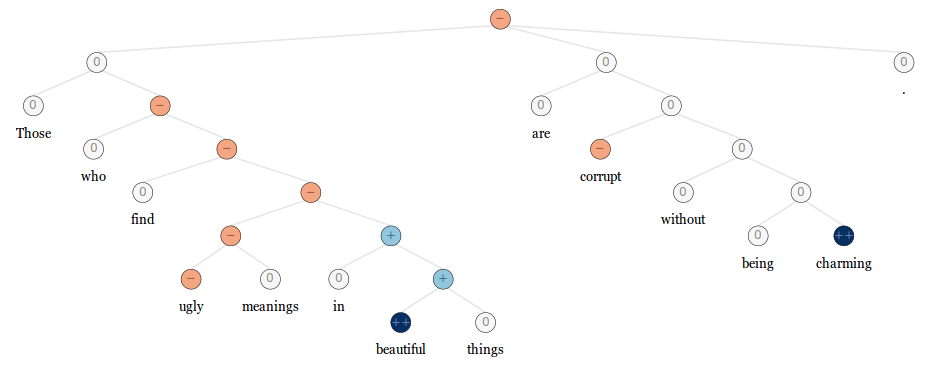
\includegraphics[scale = 0.6]{sentiment_treebank.png}
		\caption{Rečenica \ti{"Those who find ugly meanings in beautiful things are corrupt without being charming."} prikazana kroz stablo parsiranja s označenim čvorovima.}
		\label{sentiment_treebank}
	\end{figure}

	Točnost ovog modela je 80.7\%, što je izuzetno visoko. Sasvim je moguće da je ovaj model statistički točniji od "ljudskog" modela, odnosno, analize sentimenta koju provode ljudi. Naime, izvedeno je više istraživanja točnosti "ljudskih" modela te je u njima točnost varirala od 70\% do najviše 90\% \cite{ogneva2010companies, grimes2010expert}. To znači da se u 70--90\% slučajeva ljudi slažu oko stava neke rečenice, dok se u ostalim slučajevima ne slažu.

\chapter{Razvoj aplikacije za karakterizaciju likova}

	\markboth{5. \ RAZVOJ APLIKACIJE ZA KARAKTERIZACIJU LIKOVA}{}


	\section{Korišteni alati}

		Temelj nad kojim smo razvijali aplikaciju za karakterizaciju likova je \ti{Stanford CoreNLP} skup alata za obradu prirodnog jezika. To je skup brojnih alata razvijen na Sveučilištu u Stanfordu. Alati su implementirani u programskom jeziku \ti{Java}, ali ih je moguće koristiti na više načina. Najjednostavniji način je pokretanje tih alata kao samostalnih aplikacija kojima se pristupa preko web preglednika. U pregledniku predajemo tekst i odabiremo obrade koje želimo provesti. Osim toga, postoje sučelja prema brojnim programskim jezicima, poput \ti{Pythona}, pomoću kojih možemo iz tog programskog jezika pozvati sučelja prema Stanfordovom alatu. Konačno, moguće je i izravno u \ti{Javi} pristupati klasama iz Stanfordovih alata, čime dobivamo potpunu integraciju korisničkog koda i koda samog alata.

		Od brojnih alata, izravno ćemo koristiti samo tri --- alate za prepoznavanje imenovanih entiteta, za razrješavanje koreferencije te za analizu sentimenta. Prvi alat se temelji na uvjetnim slučajnim poljima, opisanim u poglavlju 2. Sljedeći alat, za razrješavanje koreferencije, koristi metodu višeprolaznog sita, opisanu na kraju poglavlja 3. Posljednji alat, za analizu sentimenta, se temelji na dubokom učenju, odnosno, rekurzivnim neuronskim mrežama, opisanim u zadnjoj sekciji poglavlja~4. Kao što smo već rekli, sva tri modela pripadaju danas najuspješnijim modelima za rješavanje danih problema.

		Osim ovih alata, \ti{Stanford CoreNLP} uključuje brojne druge, poput tokenizatora, koji rastavlja tekst na zasebne riječi (tokene), parsera gramatičke strukture rečenica ili označivača vrste riječi u rečenici. Mnoge od tih alata ćemo koristiti posredno. Na primjer, za analizu sentimenta dubokim učenjem je preduvjet odrediti gramatičku strukturu rečenice, a jedan od preduvjeta za to je prepoznati sve tokene u danoj rečenici. Dovoljno je sustavu predati popis potrebnih alata, te će \ti{Stanford CoreNLP} automatski provesti sve korake u traženom redoslijedu.

		Koristimo posljednju verziju alata, a to je 3.6.0.

		\bigskip

		%%% PROBLEM: Treba li Maven u literaturu?%%%
%%%%%
% Singer: Ne treba, link u tekstu je ok.
%%%%%
		Rješenje je implementirano u programskom jeziku Java. Za izgradnju aplikacije iz izvornog koda smo koristili sustav \ti{Gradle}. \ti{Gradle} omogućuje prilično jednostavnu i brzu izgradnju. Naime, ukoliko je potrebno koristiti dodatne biblioteke, dovoljno ih je potražiti na web stranici \href{http://mvnrepository.com/}{\ti{Maven Repository}}, odabrati verziju te dobivene podatke navesti unutar \texttt{build.gradle} dokumenta u odgovarajućoj sekciji. "Osvježavanjem" \ti{Gradle} sustava se automatski dohvaćaju \ti{Stanford CoreNLP} biblioteka i njezini već istrenirani modeli.

		Nadalje, korištena je biblioteka \texttt{sl4j} za logiranje, odnosno, ispis trenutnog stanja u konzolu, odnosno, tekstualnu (takozvanu \ti{log}) datoteku. Biblioteka se koristi i unutar \ti{Stanford CoreNLP} biblioteke za istu svrhu.

		Slijedi isječak iz \texttt{build.gradle} datoteke:

		\begin{lstlisting}
			dependencies {
				compile group: 'edu.stanford.nlp', name: 'stanford-corenlp', version: '3.6.0'
				compile group: 'edu.stanford.nlp', name: 'stanford-corenlp', version: '3.6.0', classifier: 'models'
			    compile group: 'org.slf4j', name: 'slf4j-simple', version: '1.7.21'
			}
		\end{lstlisting}

		\bigskip

		Kao razvojno okruženje koristili smo \ti{IntelliJ IDEA}, integrirano razvojno okru\-že\-nje za programski jezik Java, koje podržava \ti{Gradle} alat i omogućuje jednostavno pokretanje \ti{Gradle} zadaća i same Java aplikacije.

		 %%% PROBLEM: Treba li možda nadodati kako se pokreće? Ja pokretah preko IntelliJ IDEA-e, ali se može i preko konzole. Ako treba dodati upute za pokretanje, pretpostavljam da je dovoljno napisati za konzolu? Ili mogu preskočiti ovaj korak?%%%
%%%%%
% Singer: Ne treba - ja bih to preskocio, inace ode vertikalni prijelom :-)
%%%%%

	\section{Organizacija projekta}

		Projekt slijedi uobičajenu organizaciju gotovo svih Java projekata. Datoteke projekta su organizirane u dva temeljna direktorija, \texttt{main} i \texttt{test}. Prvi direktorij sadrži temeljni dio aplikacije nužan za rad, dok se u potonjem direktoriju nalaze podaci za testiranje rada aplikacije.

		U direktoriju \texttt{main} se nalaze direktoriji \texttt{java} i \texttt{resources}. Njihova uloga jasna je iz naziva --- \texttt{java} direktorij sadrži programski kod, odnosno, klase organizirane u pakete. S druge strane, u \texttt{resources} direktoriju se nalaze različiti dokumenti potrebni za rad aplikacije.

		Direktorij \texttt{test} sadrži samo jedan direktorij, \texttt{resources}, u kojem se pak nalazi direktorij \texttt{stories}. Ondje se nalaze odabrane dječje priče nad kojima smo testirali rad aplikacije.

		\bigskip

		Programski kod je organiziran u klase. Klase su dalje grupirane po ulozi u različite pakete:
		\begin{itemize}
			\item	paket \texttt{trainer}, u kojem se nalazi klasa \texttt{CharacterRecogniserTrainer} koja provodi treniranje novog NER modela,

			\item 	paket \texttt{solver}, u kojemu se nalazi istoimena klasa koja provodi analizu priče od početka do kraja,

			\item 	paket \texttt{phase}, u kojem se nalaze klase za svaku od tri faze našeg rješenja, \texttt{CharacterRecognition}, \texttt{CoreferenceResolution} i \texttt{SentimentAnalysis},

			\item 	paket \texttt{model}, koji sadržava klase za čuvanje podataka, u svrhu lakše obrade teksta --- \texttt{StoryData} i \texttt{CharacterName},

			\item	paket \texttt{util}, u kojem se nalazi klasa \texttt{Constants} u kojoj su pohranjene konstante, poput lokacije priča, istreniranih modela i slično.
		\end{itemize}

		Osim navedenih klasa, imamo i klasu \texttt{MainClass} koja se ne nalazi u niti jednom paketu. Ova klasa sadržava istoimenu metodu, pokretanjem koje započinjemo izvršavanje programa.

		\bigskip

		Nadalje, resursi su organizirani u dva direktorija --- \texttt{stanford} i \texttt{stories}. U prvom direktoriju se nalaze različiti dokumenti potrebni za rad \ti{Stanford CoreNLP} alata. To su:

		\begin{itemize}
			\item 	\texttt{coref-animate.txt}, koji sadržava listu svih entiteta koje će sustav za razrješavanje koreferencije smatrati živim entitetima i za koje će provoditi navedeni postupak,

			\item	\texttt{ner-training-data.tsv} i \texttt{ner-training-data-no-punctuation.tsv}, koji čini skup podataka za treniranje novog NER modela koji će moći prepoznavati likove u tekstu,

			\item 	\texttt{ner-training.properties}, u kojem su zapisane postavke samog treniranja NER modela,

			\item 	\texttt{ner-model.ser.gz} i \texttt{ner-model-no-punctuation}, koji predstavljaju pohranjene NER modele, čime izbjegavamo potrebu da svaki put prilikom pokretanja aplikacije treniramo model otpočetka.
		\end{itemize}

		Kasnije ćemo detaljnije opisati značenje i upotrebu gore navedenih datoteka.


		%%% PROBLEM: Tek naknadno uočavam grozno formatiran naslov na vrhu stranice. Micanje \\textttt ne pomaže.%%%
%%%%%
% Singer: Dodao \markright u kojem je \hbox. Napravio isto za sve \section s imenima klasa.
%   Nazalost, to ide samo rucno - grubim metodama (inace moram svasta mijenjati u styleu).
%%%%%
	\section{Klasa \texttt{MainClass}}
	\markright{5.3. \ KLASA\/ \,\hbox{\texttt{MainClass}}}

		Posebnost Java programskog jezika je u tome što sav kod mora biti organiziran u klase, te mora postojati metoda \texttt{main()} u nekoj od klasa. Pozivom ove metode započinje izvršavanje naše aplikacije. Nadalje, zbog preglednosti koda, sve važne obrade nad pričom su izdvojene u zasebne klase. U klasi \texttt{MainClass} je implementiran isključivo uvodni korak --- treniranje NER modela ukoliko on ne postoji, rad s tekstualnim datotekama i komunikacija s korisnikom.

		Prije samog koda, napomenimo da se nudi mogućnost treniranja NER modela s podacima koji sadržavaju interpunkcijske znakove, kao i s podacima iz kojih su takvi znakovi izbačeni. Detaljnije o tome ćemo reći kasnije.

		\begin{lstlisting}
		public static void main(String... args) {

			Solver solver = new Solver();
			Scanner scanner = new Scanner(System.in);
			boolean usePunctuation;

			// first step - decide type of NER classifier to use
			if (!Files.exists(Paths.get(modelLocation))) {
				trainNewCharacterRecogniser(usePunctuation);
			} else {
				System.out.println("Existing NER model for character recognition found. \n" +
						"Do you want to train new model or use old model? \n" +
						"Please enter 'y' if you want to train new model or 'n'" + "if you want to skip training.\n" +
						"If you want to exit, type 'q'.");

				while (true) {
					String input = scanner.next();
					String trimmedInput = input.trim();
					if (trimmedInput.equalsIgnoreCase("q")) {
						return;
					} else if (trimmedInput.equalsIgnoreCase("y")) {
						trainNewCharacterRecogniser(usePunctuation);
						break;
					} else if (trimmedInput.equalsIgnoreCase("n")) {
						break;
					} else {
						System.out.println("Please enter 'y', 'n' or 'q'.");
					}
				}
			}

			String modelLocation;
			if (usePunctuation) {
				modelLocation = NER_MODEL;
			}
			else {
				modelLocation = NER_MODEL_NO_PUNCTUATION;
			}

			// second step - check if NER classifier exists
			if (Files.exists(Paths.get(modelLocation))) {
				System.out.println("Existing NER model for character recognition found. Do you want to use this model or train new model? Please enter 'u' (use), 't' (train) or 'q' (exit).");

				while (true) {
					String input = scanner.next();
					String trimmedInput = input.trim();
					if (trimmedInput.equalsIgnoreCase("q")) {
						return;
					} else if (trimmedInput.equalsIgnoreCase("u")) {
						break;
					} else if (trimmedInput.equalsIgnoreCase("t")) {
						trainNewCharacterRecogniser(usePunctuation);
						break;
					} else {
						System.out.println("Please enter 'u', 't' or 'q'.");
					}
				}
			} else {
				trainNewCharacterRecogniser(usePunctuation);
			}

			// third step - solve for story
			System.out.println("Please enter file name without extension from '/src/main/resources/stories/', e.g. 'snowwhite if file name is snowwhite.txt. File should contain only story text, no titles, footnotes etc.\n If you want to exit, type 'q'.");

			while (true) {
				String input = scanner.next();
				String trimmedInput = input.trim();
				if (trimmedInput.isEmpty()) {
					System.out.println("Filename must not be empty.");
					continue;
				}
				if (trimmedInput.equalsIgnoreCase("q"))
					return;

				String storyPath = STORIES_LOCATION + input + TXT;
				if (!Files.exists(Paths.get(storyPath))) {
					System.out.println("File does not exist! Please enter existing filename.");
					continue;
				}

				try {
					solver.solveForStory(storyPath, usePunctuation);
				} catch (IOException e) {
					System.out.format("Error while reading file: %s", e.getMessage());
				}
				System.out.println("\n\n");
				System.out.println("Enter next file name or 'q' to exit.");
			}
		}
		\end{lstlisting}

		Metoda \;\texttt{trainNewCharacterRecogniser(boolean usePunctuation)}\; je po\-moć\-na metoda kojom započinjemo treniranje novog NER modela:

		\begin{lstlisting}
		private static void trainNewCharacterRecogniser(usePunctuation) {
			CharacterRecogniserTrainer trainer = new CharacterRecogniserTrainer();
			trainer.train(usePunctuation);
		}
		\end{lstlisting}

		\newpage

%%%%%
% Singer: Zbog \newpage ispred, \markright mora JOS i ISPRED naslova (LaTeX glupost).
%%%%%
	\markright{5.4. \ KLASA\/ \,\hbox{\texttt{CharacterRecogniserTrainer}}}
	\section{Klasa \texttt{CharacterRecogniserTrainer}}
	\markright{5.4. \ KLASA\/ \,\hbox{\texttt{CharacterRecogniserTrainer}}}

		Prva klasa koja će se pozvati je \texttt{CharacterRecogniserTrainer} unutar paketa \texttt{ner}. Klasa sadrži metodu \texttt{train(boolean usePunctuation)} u kojoj je implementirano treniranje novog NER modela nad zadanim podacima za učenje. Ti podaci se nalaze u direktoriju \texttt{resources/stanford} u datotekama \texttt{ner-training-data.tsv} i \texttt{ner-training-data-no-punctuation.tsv}. Prva datoteka označava podatke za učenje u kojima sam token može biti neki interpunkcijski znak. Druga datoteka pak označava iste podatke, ali iz kojih su izbačeni interpunkcijski znakovi.

		%%% PROBLEM: Kako da se najbolje (najkorektnije) pozovem na sljedeći projekt, koliko detaljno?%%%
%%%%%
% Singer: Tocno ovako kako pise :-)
%%%%%

%%%%%
% Singer: U sljedecem paragrafu, je li $F_2$ ili $F_1$ mjera???
%%%%%
		Podaci su dobiveni ručnim označavanjem ukupno $69$ dječjih priča, koje smo proveli kolega Tomislav Horina i ja, u sklopu projekta \ti{Ekstrakcija likova iz kratkih priča} na kolegiju Strojno učenje. Cilj projekta je bio istrenirati više NER modela koji će uspješno prepoznavati (imenovane i neimenovane) likove u danim pričama --- bajkama, basnama, mitovima i legendama. Modeli su se temeljili na skrivenim Markovljevim modelima, uvjetnim slučajnim poljima te na \ti{Stanford NER} sustavu. Najkvalitetniji modeli su dobiveni upravo treniranjem vlastitog \ti{Stanford NER} modela, te je njihova $F_2$ mjera iznosila oko $0.6$. Prilikom testiranja, model treniran nad podacima koji ne uključuju interpunkcijske znakove je pokazivao neznatno bolje rezultate.

		Prvi korak projekta je bila priprema podataka za učenje. S web-stranice \ti{Project Gutenberg} je prikupljen veći broj priča. Za svaku priču je automatski generirana po jedna \texttt{tsv} (\ti{tab separated value}) datoteka dvostupčanog formata, pri čemu su u drugom stupcu, redom, tokeni te priče, dok je u prvom stupcu oznaka klase kojoj pripada taj token. Oznaka je \texttt{C} (\ti{character}) ukoliko se radi o liku, inače je oznaka \texttt{O} (\ti{other}).

		Sljedeći tekst je isječak iz datoteke \texttt{ner-training-data.tsv} koja sadrži interpunkcijske znakove:

		\begin{lstlisting}
			O	Long
			O	ago
			O	there
			O	lived
			O	a
			O	monarch
			O	,
			O	who
			O	was
			O	such
			O	a
			O	very
			O	honest
			O	man
			O	that
			O	his
			O	subjects
			O	entitled
			O	him
			O	the
			C	Good
			C	King
			O	.
		\end{lstlisting}

		S druge strane, ovo je analogni isječak iz datoteke \texttt{ner-training-data.tsv}, u kojoj su regularnim izrazima izbačeni svi interpunkcijski znakovi:

%%%%%
% Singer: Dodao po jedan TAB u svaki red, da izgleda isto kao gore :-)
%%%%%
		\begin{lstlisting}
			O	Long
			O	ago
			O	there
			O	lived
			O	a
			O	monarch
			O	who
			O	was
			O	such
			O	a
			O	very
			O	honest
			O	man
			O	that
			O	his
			O	subjects
			O	entitled
			O	him
			O	the
			C	Good
			C	King
		\end{lstlisting}

		U generiranoj datoteci su, u početku, svi tokeni nosili oznaku \texttt{O}\@. Čitanjem priča smo kolega i ja uočavali likove te oznake pripadnih tokena mijenjali u \texttt{C}\@. Potom su sve datoteke spojene u jedinstvenu datoteku čija duljina je preko dvjesto tisuća linija. Također je stvorena kopija te datoteke, iz koje su regularnim izrazima uklonjeni svi retci koji sadrže interpunkcijske znakove. Te datoteke su činile skup podataka za treniranje NER modela.

		Pri treniranju novog \ti{Stanford NER} modela, osim datoteke s podacima za učenje, potrebno je predati i \texttt{ner-trainer.properties} datoteku. U njoj su zadane postavke treniranja, poput poretka stupaca u tim podacima i duljine n-grama koji će se promatrati pri treniranju. Korištene su preporučene postavke:

		\begin{lstlisting}
			map = word=1,answer=0
			useClassFeature=true
			useWord=true
			useNGrams=true
			noMidNGrams=true
			maxNGramLeng=6
			usePrev=true
			useNext=true
			useSequences=true
			usePrevSequences=true
			maxLeft=1
			useTypeSeqs=true
			useTypeSeqs2=true
			useTypeySequences=true
			wordShape=chris2useLC
			useDisjunctive=true
			saveFeatureIndexToDisk=true
		\end{lstlisting}

		Ova datoteka se, također, nalazi u direktoriju \texttt{resources/stanford}.

		\bigskip

		Slijedi programski kod klase \texttt{CharacterRecogniserTrainer}:

		\begin{lstlisting}
			public class CharacterRecogniserTrainer {

				private Logger logger = LoggerFactory.getLogger(CharacterRecogniserTrainer.class);

				public void train(boolean usePunctuation) {

					logger.info("Started training of new NER model. Model includes punctuation: {}", includePunctuation);

					Properties properties = StringUtils.propFileToProperties(TRAINING_PROPERTIES);
					if (includePunctuation) {
						properties.setProperty(TRAIN_FILE, TRAINING_DATA);
						location = NER_MODEL;
					}
					else {
						properties.setProperty(TRAIN_FILE, TRAINING_DATA_NO_PUNCTUATION);
						location = NER_MODEL_NO_PUNCTUATION;
					}
					SeqClassifierFlags flags = new SeqClassifierFlags(properties);
					CRFClassifier<CoreLabel> crf = new CRFClassifier<>(flags);
					crf.train();
					crf.serializeClassifier(location);
					logger.info("Training finished. Model saved to {}.", NER_MODEL);
				}
			}
		\end{lstlisting}

		Nakon učitavanja \texttt{training.properties} datoteke, njezine vrijednosti se postavljaju kao postavke treniranja. Također se, ovisno o korisnikovom odabiru modela, postavlja lokacija gdje će se pohraniti istrenirani model. To je jedna od sljedećih lokacija:
		\begin{itemize}
			\item 	 \texttt{resources/stanford/ner-model.ser.gz}
			\item 	 \texttt{resources/stanford/ner-model-no-punctuation.ser.gz}
		\end{itemize}

%%%%%
% Singer: Na pocetku druge recenice, promijenio "Konačno" u "Zatim", da ne javlja overfull \hbox.
%%%%%
		Naredbom \texttt{crf.train(boolean usePunctuation)} započinjemo treniranje klasifikatora sa zadanim postavkama. Zatim, naredbom \texttt{crf.serializeClassifier (SERIALIZE\_LOCATION)} pohranjujemo istrenirani klasifikator na zadanu lokaciju.


	\section{Klase \texttt{StoryData} i \texttt{CharacterName}}
	\markright{5.5. \ KLASE\/ \,\hbox{\texttt{StoryData\/}} I\/ \,\hbox{\texttt{CharacterName}}}

		Ove dvije klase predstavljaju pomoćne klase za pohranu podataka o samoj priči i likovima. Nalaze se u paketu \texttt{model}.

		Klasu \texttt{StoryData} čine varijable \texttt{characters}, odnosno, popis likova prepoznatih u priči, te sam tekst priče \texttt{story}. Osim njih, imamo i metode za postavljanje i dohvaćanje njihovih vrijednosti, takozvane \ti{gettere} i \ti{settere}.

		\begin{lstlisting}
		public class StoryData {

			private List<CharacterName> characters;
			private String story;



			public List<CharacterName> getCharacters() {
				return characters;
			}

			public void setCharacters(List<CharacterName> characters) {
				this.characters = characters;
			}

			public String getStory() {
				return story;
			}

			public void setStory(String story) {
				this.story = story;
			}
		}
		\end{lstlisting}

%%%%%
% Singer: Dodao malo vertikalnog razmaka, da ne javlja underfull \vbox.
%%%%%
		\vspace*{6pt}
		Klasa \texttt{CharacterName} predstavlja nešto složeniji prikaz imena pojedinog lika. Naime, likovi često imaju složeno ime koje se sastoji od više riječi, na primjer \textit{mother goat} u \ti{Vuku i sedam kozlića}. Sasvim je moguće da se autor na takve likove ponekad referira punim imenom, a ponekad skraćenim imenom, na primjer \textit{mother}. S obzirom da bismo htjeli prepoznati navedenog lika u svim situacijama, osim njegovog punog imena (\texttt{fullName}), čuvamo i skup samih riječi (\texttt{tokens}):

		\begin{lstlisting}
		public class CharacterName {

			private String fullName;

			private List<String> tokens;

			public CharacterName(String fullName, List<String> tokens) {
				this.fullName = fullName;
				this.tokens = tokens;
			}

			public String getFullName() {
				return fullName;
			}

			public void setFullName(String fullName) {
				this.fullName = fullName;
			}

			public List<String> getTokens() {
				return tokens;
			}

			public void setTokens(List<String> tokens) {
				this.tokens = tokens;
			}

			@Override
			public String toString() {
				return "Full name: " + fullName + ", tokens: " + tokens.toString();
			}
		}
		\end{lstlisting}

		Metoda \texttt{toString()} omogućuje jasniji ispis objekata ove klase.

	\section{Klasa \texttt{Solver}}
	\markright{5.6. \ KLASA\/ \,\hbox{\texttt{Solver}}}

		Klasa \texttt{Solver} čini srž naše aplikacije. U njoj se provodi analiza čitave priče, odnosno, tri prethodno opisana koraka.

%%%%%
% Singer: Dodao malo vertikalnog razmaka, da ne javlja underfull \vbox.
%%%%%
		\vspace*{6pt}
		Jedina metoda koju ova klasa sadrži je \texttt{solveForStory(String path, \!boolean usePunctuation)}, koja prima lokaciju priče koju želimo analizirati i podatak o tome koji NER model koristimo. Priča treba biti u tekstualnoj (\texttt{.txt}) datoteci, te bi trebala sadržavati isključivo tekst same priče, bez naslova, bilješki, komentara i sličnog dodatnog teksta.

		\begin{lstlisting}

		public class Solver {

			private CharacterRecognition characterRecognition = new CharacterRecognition();

			private CoreferenceResolution coreferenceResolution = new CoreferenceResolution();

			private SentimentAnalysis sentimentAnalysis = new SentimentAnalysis();


			public void solveForStory(String path, boolean usePunctuation) throws IOException {

				StoryData storyData = characterRecognition.setUpStoryAndCharacters(path, usePunctuation);
				List<String> characterTextList = coreferenceResolution.recogniseCharacterSentences(storyData);
				List<String> sentiments = sentimentAnalysis.calculateCharacterSentiments(
				characterTextList);
				System.out.println("-------------------------------------------");
				System.out.println("Results:");
				for (int i = 0; i < sentiments.size(); ++i) {
					System.out.format("%s: %s\n", storyData.getCharacters().get(i).getFullName(), sentiments.get(i));
				}
				System.out.println("------------------------------------------");
			}
		}
		\end{lstlisting}

		Kao što vidimo, prvi korak je postavljanje \texttt{storyData} varijable kroz metodu \texttt{setUpStoryAndCharacters(String path, \!boolean useInterpunction)} iz klase \texttt{CharacterRecognition}. U toj metodi se ekstrahiraju likovi i tekst priče. Sljedeći korak je prepoznavanje onih rečenica u priči koje se odnose na pojedinog lika. Ovaj postupak je implementiran u metodi \texttt{recogniseCharacterSentences(StoryData storyData)} iz klase \texttt{CoreferenceResolution}. Rezultat je lista tekstova koji su potom dani, kao ulaz, metodi \texttt{calculateCharacterSentiments(List<String> characterSentences)}, koja obavlja analizu sentimenta nad svakim od njih. Ta metoda se nalazi u klasi \texttt{SentimentAnalysis}. Sve tri navedene klase se nalaze u zasebnom paketu \texttt{phase}.

		Napomenimo još samo da se razrješavanje koreferencije i analiza sentimenta ponašaju jednako, neovisno o tome koji NER model koristimo. NER model utječe samo na prvi korak, prepoznavanje samih likova u priči.

		\newpage

	\section{Klasa \texttt{CharacterRecognition}}
	\markright{5.7. \ KLASA\/ \,\hbox{\texttt{CharacterRecognition}}}

		U ovoj klasi implementiramo prepoznavanje likova u priči, odnosno, popunjavanje \texttt{StoryData} varijable. Glavna metoda u klasi je \texttt{setUpStoryAndCharacters}:

		\begin{lstlisting}
		public StoryData setUpStoryAndCharacters(String path,
												boolean modelWithPunctuation)
			throws IOException
		{

			// load NER model
			NERClassifierCombiner classifier;
			if (modelWithPunctuation) {
				classifier = new NERClassifierCombiner(false, false, NER_MODEL);
			}
			else {
				classifier = new NERClassifierCombiner(false, false, NER_MODEL_NO_PUNCTUATION);
			}
			// read story text
			String storyText = IOUtils.slurpFile(path);

			// tag story with NER tags
			List<List<CoreLabel>> taggedText = classifier.classify(storyText);
			List<CharacterName> characters = new ArrayList<>();

			for (List<CoreLabel> sentence : taggedText) {
				for (int i = 0; i < sentence.size(); ++i) {
					CoreLabel firstLabel = sentence.get(i);
					String tag = firstLabel.ner();
					String name = firstLabel.value();
					if (tag.equals("O")) {
						continue;
					}

					List<String> tokens = new ArrayList<>();
					tokens.add(name.toLowerCase());
					CoreLabel nextLabel = sentence.get(i + 1);

					// read all neighbouring character tokens
					// they all belong to single character

					while (nextLabel.ner().equals("C")) {
						name += " " + nextLabel.value();
						tokens.add(nextLabel.value().toLowerCase());
						++i;
						if (i >= sentence.size() - 1) {
							break;
						}
						nextLabel = sentence.get(i + 1);
					}
					updateCharacterList(name, tokens, characters);
				}
			}

			StoryData storyData = new StoryData();
			storyData.setCharacters(characters);
			storyData.setStory(storyText);
			logger.info("File '{}' successfully read.", path);
			logger.info("Found characters:\n{}", buildNiceCharactersString(characters));
			return storyData;
		}
		\end{lstlisting}

%%%%%
% Singer: Dodao malo vertikalnog razmaka, da ne javlja underfull \vbox.
%%%%%
		\vspace*{1pt}
		Dakle, prvi korak je učitavanje NER modela i njegovo pokretanje nad tekstom. Rezultat je lista rečenica, od kojih se svaka sastoji od liste \texttt{CoreLabel} objekata. \texttt{CoreLabel} klasa dolazi iz \ti{Stanford CoreNLP} biblioteke, te označava jedan obrađeni token. Potom, iteriramo po označenim rečenicama i unutar njih tražimo tokene označene oznakom \texttt{C}\@. Kada naiđemo na takav token, varijabli \texttt{name} pridružujemo njezinu vrijednost. Također, dodajemo vrijednost tokena u skup \texttt{tokens}. Nakon toga provjeravamo je li sljedeći token, također, označen tom klasom. Ukoliko jest, proširujemo ime lika novim tokenom, te dodajemo novi token u skup. Postupak ponavljamo dokle god je oznaka jednaka \texttt{C}\@. S obzirom da većina likova ima imena od jedne ili dvije riječi, očekujemo jednako toliko ponavljanja.

		Na kraju iteracije imamo puno ime pronađenog lika, kao i potpunu listu tokena. S obzirom da se imena likova ponavljaju u tekstu, te da se likovi mogu oslovljavati punim imenom, kao i skraćenim, potrebno je provjeriti možemo li dodati novog lika u popis likova ili se pak radi o postojećem liku. Za svakog lika provjeravamo sadrži li novodobivena lista tokena sve njegove tokene. Ako sadrži, nadopunjujemo ime postojećeg lika. Ako ne sadrži, provjeravamo obratnu situaciju, odnosno, sadrže li postojeći tokeni sve nove tokene. U tom slučaju, pronašli smo samo dio imena nekog lika i vraćamo se u glavnu metodu bez ikakvih promjena nad listom likova. U metodi su u komentarima dani primjeri iz kojih je jasnije.

		Konačno, u trećem slučaju, kada su skupovi tokena svih dosad prepoznatih likova posve disjunktni s pronađenim tokenima, očito, imamo posve novog, nepoznatog lika kojeg je potrebno dodati u listu.

		Gore opisan postupak je implementiran u zasebnoj metodi:

		\begin{lstlisting}
		private void updateCharacterList(String name,
														List<String> tokens,
														List<CharacterName> characters) {
			for (CharacterName character : characters) {
				// already in list: Red Riding Hood
				// now found: Little Red Riding Hood
				// update character name
				if (tokens.containsAll(character.getTokens())) {
					character.setFullName(name);
					character.setTokens(tokens);
					return;
				}
				// opposite:
				// already in list: Little Red Riding Hood
				// now found: Red Riding Hood
				// skip
				if (character.getTokens().containsAll(tokens)) {
					return;
				}
			}
			// other situation - completely new character
			CharacterName newCharacter = new CharacterName(name, tokens);
			characters.add(newCharacter);
		}
		\end{lstlisting}

		Na samom kraju metode \texttt{setUpStoryData} postavljamo varijablu \texttt{storyData}, ispisujemo poruku o uspješno završenom postupku, kao i popis prepoznatih likova. Metoda \texttt{buildNiceCharactersString} za cilj ima generirati pregledan zapis liste likova.

		\newpage

	\markright{5.8. \ KLASA\/ \,\hbox{\texttt{CoreferenceResolution}}}
	\section{Klasa \texttt{CoreferenceResolution}}
	\markright{5.8. \ KLASA\/ \,\hbox{\texttt{CoreferenceResolution}}}

		U ovoj klasi je implementiran sljedeći korak, razrješavanje koreferencije, odnosno, prepoznavanje onih rečenica u priči koje pripadaju pojedinom liku. Glavna metoda je \texttt{recogniseCharacterSentences}:

		\begin{lstlisting}
		public List<String> recogniseCharacterSentences(StoryData storyData) {

			// set up annotator
			StanfordCoreNLP pipeline = setUpCoreferencePipeline();
			Annotation document = pipeline.process(storyData.getStory());

			int numberOfCharacters = storyData.getCharacters().size();
			List<String> characterTextList = initializeAllCharacterTexts(numberOfCharacters);
			List<CoreMap> sentences = document.get(SentencesAnnotation.class);

			for (CorefChain cc : document.get(CorefChainAnnotation.class).values()) {
				List<CorefChain.CorefMention> mentions = cc.getMentionsInTextualOrder();
				logger.info("Mentions in current chain: {}", mentions);

				int characterIndex = checkMentionChainForAnyCharacter(storyData, mentions);
				if (characterIndex == -1) {
					// character not found in current mention chain
					continue;
				}
				updateCharacterTextList(characterIndex, characterTextList, sentences, mentions);
			}
			return characterTextList;
		}
		\end{lstlisting}

		U metodi prvo postavljamo objekt klase \texttt{StanfordCoreNLP}, kroz kojega ćemo pozvati razrješavanje koreferencije, i to kroz sljedeću metodu:

		\begin{lstlisting}
		private StanfordCoreNLP setUpCoreferencePipeline() {
			Properties props = new Properties();
			props.setProperty("annotators", "tokenize, ssplit, pos, lemma, ner, parse, mention, dcoref");
			props.setProperty("dcoref.use.big.gender.number", "false");
			props.setProperty("dcoref.animate", ANIMATE_LIST);
			return new StanfordCoreNLP(props);
		}
		\end{lstlisting}

		Postavljamo preporučene postavke, osim za popis živih entiteta, gdje zadajemo vlastitu listu, koju čine lista i živih i neživih entiteta. Bez te promjene, sustav za razrješavanje koreferencije ne provodi taj postupak za nežive entitete, poput mački, ogledala, patuljaka. Drugim riječima, u sljedećem primjeru, sustav ne bi prepoznao da se \ti{she} odnosi na \ti{cat}: \ti{"Cat is on the mat. She is sleeping."}

		\bigskip

		U metodi \texttt{initializeAllCharacterTexts}, za početak, inicijaliziramo tekstove svih likova na prazne nizove.

		Sljedeći korak je obrada teksta, odnosno, provođenje samog postupka raz\-rje\-ša\-va\-nja koreferencije nad pričom. Time smo dobili listu rečenica \texttt{sentences}, ali i listu svih \texttt{CorefChain} objekata, koje čini niz prepoznatih međusobno koreferentnih izraza u tekstu. Jedan primjer tog objekta je:

		\begin{lstlisting}
		[a huntsman" in sentence 15, "The huntsman" in sentence 17, "he" in sentence 17, "his" in sentence 17, "my" in sentence 17, "I" in sentence 17, "the huntsman" in sentence 18, "he" in sentence 18, "the huntsman" in sentence 49, "the huntsman" in sentence 57]
		\end{lstlisting}

		Iteriramo kroz sve \texttt{CorefChain} objekte. U svakoj iteraciji provjeravamo spominje li se neki od likova u tom lancu koreferentnih izraza. Ako se spominje, dohvaćamo njegov indeks:

		\begin{lstlisting}
		private int checkMentionChainForAnyCharacter(StoryData storyData,
																 List<CorefMention> mentions) {

			int numberOfCharacters = storyData.getCharacters().size();
			for (CorefMention mention : mentions) {
				for (int i = 0; i < numberOfCharacters; ++i) {
					for (String characterToken : storyData.getCharacters().get(i).getTokens()) {

						// get all words in single mention
						// example of mention:
						// "dwarves, which were living in the mountains"
						String[] mentionWords = mention.mentionSpan.split("[\\.\\'\\,\\ ]+");
						for (String mentionWord : mentionWords) {
							if (equalsIgnoreCase(mentionWord, characterToken)) {
								logger.info("Found character {} in mention '{}', mention chain is '{}'",
								storyData.getCharacters().get(i).getFullName(),
								mention.mentionSpan,
								mentions);
								return i;
							}
						}
					}
				}
			}
			return -1;
		}
		\end{lstlisting}

		Dakle, ako je indeks različit od $-1$, nadopunjemo tekst koji se odnosi na tog lika:

		\begin{lstlisting}

		private void updateCharacterTextList(int characterIndex,
																List<String> characterTextList,
																List<CoreMap> sentences,
																List<CorefMention> mentions) {

			for (CorefMention mention : mentions) {
				// check if character is subject in that sentence
				CoreMap coreMap = sentences.get(mention.sentNum - 1);
				String characterText = characterTextList.get(characterIndex);

				// there can be multiple mentions in same sentence
				// if that case, such sentences would be added multiple times, once for every mention
				if (characterText.contains(coreMap.toString())) {
					return;
				}

				SemanticGraph semanticGraph = coreMap.get(CollapsedCCProcessedDependenciesAnnotation.class);
				IndexedWord verb = semanticGraph.getFirstRoot();
				IndexedWord subject = semanticGraph.getChildWithReln(verb,
				GrammaticalRelation.valueOf(Language.UniversalEnglish, "nsubj"));


				// if subject is not found or if character is subject
				// add that sentence to text
				// very often, characters are both subjects and objects
				// we want only subjects - bad characters often do something
				// bad to another character
				// both bad and good characters would get that same bad sentence
				if (subject == null ||
						containsIgnoreCase(mention.mentionSpan, subject.word())) {
					String updatedText = characterText + " " + coreMap;
					characterTextList.set(characterIndex, updatedText);
				}
			}
		}
		\end{lstlisting}

		U gornjoj metodi iteriramo po koreferentnim izrazima u lancu. U prvom koraku provjeravamo nalazi li se već u tekstu rečenica u kojoj se nalazi koreferentni izraz. Ako je odgovor potvrdan, nije ju potrebno dodavati, s obzirom da ne želimo da ista rečenica više puta sudjeluje u analizi sentimenta, već samo jednom.

		U sljedećem koraku dohvaćamo subjekt dane rečenice i provjeravamo je li subjekt dio koreferentnog izraza. Ovaj korak je dodan kao neplanirana optimizacija, s obzirom se u istoj rečenici mogu spominjati dva lika, jedan kao subjekt, a drugi kao objekt. U tom slučaju, najčešće, želimo tu rečenicu pridružiti liku koji je subjekt, a ne objekt. Naime, često zločesti likovi, kao subjekti u rečenici, vrše neku negativnu radnju (na primjer, vrijeđanje) nad dobrim likom, koji je objekt. Bez prepoznavanja subjekta, negativnu rečenicu bismo pridružili i pozitivnom i negativnom liku. Ipak, ponekad analiza rečenice ne uspije pronaći subjekt. U toj situaciji rečenicu ipak pridružujemo liku.

	\markright{5.9. \ KLASA\/ \,\hbox{\texttt{SentimentAnalysis}}}
	\section{Klasa \texttt{SentimentAnalysis}}
	\markright{5.9. \ KLASA\/ \,\hbox{\texttt{SentimentAnalysis}}}

		Ova klasa čini zadnji korak analize priče, odnosno, čitavog algoritma. Temeljna metoda u njoj je  \texttt{calculateCharacterSentiments}, koja, za sve likove, izračunava pripadni sentiment:

		\begin{lstlisting}
		public List<String> calculateCharacterSentiments(List<String> characterTextList) {

			StanfordCoreNLP pipeline = setUpSentimentPipeline();
			logger.info("Calculating sentiment for each character...");
			List<String> sentiments = new ArrayList<>();

			for (String text : characterTextList) {
				String sentiment = calculateSentiment(pipeline, text);
				sentiments.add(sentiment);
			}
			return sentiments;
		}
		\end{lstlisting}

%%%%%
% Singer: Dodao malo vertikalnog razmaka, da ne javlja underfull \vbox.
%%%%%
		\vskip 6pt plus 2pt minus 1pt
		Slično kao i u klasi \texttt{CoreferenceResolution}, prvi korak je postavljanje \texttt{Stan\-ford CoreNLP} objekta, koji će provesti analizu sentimenta:

		\begin{lstlisting}
		private StanfordCoreNLP setUpSentimentPipeline() {
			Properties sentProperties = new Properties();
			sentProperties.setProperty("annotators", "tokenize, ssplit, pos, parse, sentiment");
			return new StanfordCoreNLP(sentProperties);
		}
		\end{lstlisting}

%%%%%
% Singer: Dodao malo vertikalnog razmaka, da ne javlja underfull \vbox.
%%%%%
		\vskip 6pt plus 2pt minus 1pt
		U sljedećem koraku iteriramo po tekstovima pojedinih likova i provodimo analizu sentimenta nad njima. U metodi \texttt{calculateSentiment}, za dani tekst, ra\-ču\-na\-mo sentiment:
		\begin{lstlisting}
		private String calculateSentiment(StanfordCoreNLP pipeline,
															String text) {

			if (text.length() == 0) {
				logger.info("Text is empty - skipping sentiment analysis.");
				return "insufficient data for sentiment analysis";
			}

			logger.info("Received text for sentiment analysis:\n{}", text.toString());

			double sum = 0;
			int count = 0;

			// predicted class can be one of:
			// O = very negative
			// 1 = negative
			// 2 = neutral
			// 3 = positive
			// 4 = very positive

			Annotation document = pipeline.process(text);

			for (CoreMap sentence : document.get(CoreAnnotations.SentencesAnnotation.class)) {
				Tree tree = sentence.get(SentimentCoreAnnotations.SentimentAnnotatedTree.class);
				int sentiment = RNNCoreAnnotations.getPredictedClass(tree);
				if (sentiment >= 0) {
					sum += sentiment;
					++count;
				}
			}

			// return average of sentence sentiments
			double value = sum / count;
			logger.info("Sentiment numeric value: {}", value);

			// usually, neutral characters are considered good
			if (value <= 1.5)
				return "bad";
			else
				return "good";
		}
		\end{lstlisting}

		Uočimo da smo odabrali karakterizirati likove isključivo kao dobre ili loše. Razlog tome je što djeca često promatraju svijet crno-bijelo. Posebno, u dječjim lektirama, u nižim razredima, gotovo uvijek se na taj način karakteriziraju likovi. Nikad nije pitanje tko je u priči neutralan lik, već tko su dobri, a tko loši likovi.

		Nadalje, Stanfordov sustav dodjeljuje sljedeće ocjene rečenicama:
		\begin{itemize}
			\item	0 --- izrazito negativna rečenica,
			\item 	1 --- negativna rečenica,
			\item 	2 --- neutralna rečenica,
			\item 	3 --- pozitivna rečenica,
			\item 	4 --- izrazito pozitivna rečenica.
		\end{itemize}

		S obzirom na to, prag od $1.5$ za lošeg lika znači da samo isključivo negativno ocijenjene likove smatramo zlima. S druge strane, neutralni likovi će često u dječjim pričama biti proglašeni dobrima. Razlog tome je crno-bijelo viđenje svijeta. Svatko, tko nije izrazito zločest, je dobar.
%%%%%
% Singer: Dodao \newpage, inace NECE :-(
%%%%%
\newpage
	\markright{5.10. \ KLASA\/ \,\hbox{\texttt{Constants}}}
	\section{Klasa \texttt{Constants}}
	\markright{5.10. \ KLASA\/ \,\hbox{\texttt{Constants}}}

		Ova klasa se nalazi u paketu \texttt{util} i sadržava tekstualne konstante:

		\begin{lstlisting}
		public class Constants {

			public static final String TRAINING_PROPERTIES = "src/main/resources/stanford/ner-training.properties";
			public static final String NER_MODEL = "src/main/resources/stanford/ner-model.ser.gz";
			public static final String NER_MODEL_NO_PUNCTUATION = "src/main/resources/stanford/ner-model-no-punctuation.ser.gz";
			public static final String STORIES = "src/main/resources/stories/";
			public static final String ANIMATE_LIST = "src/main/resources/stanford/coref-animate.txt";
			public static final String TXT = ".txt";
			public static final String TRAINING_DATA = "src/test/resources/stanford/ner-training-data.tsv";
			public static final String TRAINING_DATA_NO_PUNCTUATION = "src/main/resources/stanford/ner-training-data-no-punctuation.tsv";
			public static final String TRAIN_FILE = "trainFile";

			private Constants() {}
		}
		\end{lstlisting}

		Svrha izdvajanja konstanti u zasebnu klasu je veća preglednost koda te izbjegavanje definiranja iste konstante u različitim klasama.

	\chapter{Rezultati}

	\markboth{6. \ REZULTATI}{}

		Aplikaciju smo testirali nad desetak dječjih priča. Za svaku od priča ćemo dati kratki sažetak s opisom likova. Nadalje, zapisat ćemo i komentirati dobivene rezultate.

		Napomenimo samo da su neke od bajki dane u svom izvornom zapisu, koji je ponešto drukčiji od modernih, nježnijih verzija tih bajki.

	\section{Pepeljuga}

		Ova priča predstavlja varijantu poznate priče o Pepeljugi.

		\subsection{Sažetak}

		Pepeljuga je djevojka, čija je majka, dobra i pobožna žena, umrla. Pepeljuga je majci na samrti obećala da će biti dobra i pobožna. Otac se nakon nekog vremena ponovno oženio, i kako to obično biva u bajkama, maćeha je bila zla žena. Imala je dvije prelijepe, ali zločeste kćeri. Jednog dana je otac išao na sajam. Kad je pitao djevojke što žele da im donese, bahate kćeri su rekle da žele skupu odjeću, dok je Pepeljuga htjela prvu granu koja dodirne lice njenog oca dok bude putovao. Otac je tako i uradio. Kad se vratio, Pepeljuga je na majčin grob zarila tu granu, nad kojom je često plakala i koja je ubrzo izrasla u prekrasno stablo. Svaki put kad bi Pepeljuga plakala pred stablom, pojavila bi se bijela golubica i ispunila bilo koju njezinu želju.

		Ubrzo je kralj odlučio organizirati trodnevni festival za sav narod, s ciljem da njegov sin nađe ženu. Pepeljugi je maćeha zabranila da ide na bal, jer je imala kućanskih poslova za obaviti, te nije imala lijepe odjeće. Pepeljuga je zazvala ptice da joj pomognu s kućanskim poslovima, te je plakala na majčinom grobu i zazivala stablo da joj donese haljinu, što se i dogodilo. Pepeljuga je bila najljepša na balu. Princ je isključivo s njom plesao i nije htio da itko drugi pleše s njom. Po završetku bala, princ ju je htio otpratiti kući, ali je Pepeljuga odlučila pobjeći od srama. Sljedeći dan se sve ponovilo --- Pepeljuga je zazvala još ljepšu haljinu, plesala s princem i pobjegla. Isto se dogodilo i posljednjeg dana, ali princ je odlučio stepenice premazati smolom, tako da se Pepeljugina cipela pri bijegu zalijepila.

		Sljedećeg dana je princ otišao k dvjema sestrama da provjeri pripada li cipela nekoj od njih dvije. Starijoj kćeri je cipela bila prevelika, pa je poslušala majčin savjet i odrezala prst, te obukla cipelu. Princ je nasjeo na prevaru, te je krenuo sa starijom sestrom prema dvorcu. Putem je uočio da joj stopalo krvari, te se vratio kući i zahtijevao da mlađa kći proba cipelu. Mlađoj kćeri, s druge strane, peta nije mogla stati u cipelu, te si je ona odrezala petu. Ponovno se dogodila ista situacija --- krenuli su prema dvorcu, ali je princ vidio da krvari i da je prevaren. Naposljetku je Pepeljuga probala cipelu te je princ shvatio da je ona njegova mladenka.

		Na dan vjenčanja, dvije sestre su hodale uz kraljevski par. Za kaznu njihovoj bahatosti i zlobi, golubovi su ih napali i oslijepili.

		\subsection{Likovi}

		Možemo zaključiti da je u ovoj priči Pepeljuga dobar lik, kao i njezina pokojna majka, te princ i otac. S druge strane, maćeha i njezine kćeri su zli likovi.

		\subsection{Dobiveni rezultati uz upotrebu NER modela s interpunkcijskim znakovima}

		\begin{verbatim}
			[main] INFO step.CharacterRecognition - Found characters:
			princess
			sisters
			bird
			King
			Aschenputtel
			mother
			step-mother
			prince
			father
			queen
		\end{verbatim}

		Očito je da sustav nije posve uspješno prepoznao likove. Princeza se odnosi na Pepeljugu na balu, kada su smatrali da je ona nepoznata princeza daleke zemlje. Ptica, odnosno, bijela golubica je, također, prepoznata kao lik. To možda i nije posve pogrešno, s obzirom da je ptica imala dosta veliku ulogu u priči --- pomagala je Pepeljugi s kućanskim poslovima, ostvarivala želje. Nadalje, kraljica se u priči spominje u dvije rečenice, a to su savjeti maćehe kćerima: \ti{Kada budeš kraljica, nećeš nikad morati pješačiti}. Vjerojatan razlog za prepoznavanje kraljice je taj što je NER sustav treniran nad većim brojem priča u kojima su kraljice bile likovi. Konačno, majka se ipak odnosi na maćehu, a ne na pokojnu majku.

		\begin{verbatim}
			Results:
			princess: good
			sisters: bad
			bird: bad
			King: bad
			Aschenputtel: bad
			mother: bad
			step-mother: insufficient data for sentiment analysis
			prince: good
			father: bad
			queen: insufficient data for sentiment analysis
		\end{verbatim}

		Sustav je ispravno prepoznao sestre kao zločeste likove, kao i majku, odnosno, maćehu. Također, kralj, princ i princeza (Pepeljuga na balu) su okarakterizirani kao dobri likovi.

%%%%%
% Singer: "je zla" -> "su zle" (mnozina).
%%%%%
		S druge strane, za pticu i samu Pepeljugu je sustav zaključio da su zle. Pro\-u\-ča\-va\-njem ispisa u konzoli uočavamo da se na Pepeljugu odnose sljedeće rečenice:

		\begin{verbatim}
			[main] INFO step.SentimentAnalysis -
			Sentence: Then the two sisters were very glad, because they had
			pretty feet.
			Sentiment: 2

			[main] INFO step.SentimentAnalysis -
			Sentence: Besides that, the sisters did their utmost to torment
			her,--mocking her, and strewing peas and lentils among the ashes,
			and setting her to pick them up.
			Sentiment: 1

			[main] INFO step.SentimentAnalysis -
			Sentence: The step-mother and the two sisters were thunderstruck,
			and grew pale with anger; but he put Aschenputtel before him on
			his horse and rode off.
			Sentiment: 1

			[main] INFO step.SentimentAnalysis -
			Sentence: And as they passed the hazel bush, the two white pigeons
			cried, "There they go, there they go!
			Sentiment: 1

			[main] INFO step.SentimentAnalysis -
			Sentence: And when her wedding with the prince was appointed to
			be held the false sisters came, hoping to curry favour, and to
			take part in the festivities.
			Sentiment: 1

			[main] INFO step.SentimentAnalysis -
			Sentence: Of Aschenputtel they never thought at all, and supposed
			that she was sitting at home, and picking the lentils out of the
			ashes.
			Sentiment: 1

			[main] INFO step.SentimentAnalysis - Final sentiment numeric value:
			1.1666666666666667
		\end{verbatim}

		Zaključujemo da je jedan od problema sustava taj što nije ispravno dodijelio rečenice likovima. Gotovo sve prethodne rečenice se odnose na Pepeljugu, ali opisuju postupke zlobnih sestara prema njoj. Dakle, bilo bi ispravno kad bi te rečenice bile dodijeljene sestrama, a ne Pepeljugi.

		Nadalje, problem predstavlja i pogrešno zaključivanje sustava za analizu sentimenta. Na primjer, tužne rečenice su uglavnom ocijenjene negativno. U dječjim pričama to može dovesti do greške, s obzirom da takve rečenice zapravo definiraju dobre likove.

		Konačno, za oca je utvrđeno da je zao:

		\begin{verbatim}
			[main] INFO step.SentimentAnalysis -
			Sentence: The father thought to himself,
			"It cannot surely be Aschenputtel," and called for axes and
			hatchets, and had the pigeon-house cut down, but there was no
			one in it.
			Sentiment: 1

			[main] INFO step.SentimentAnalysis -
			Sentence: "The first twig, father, that strikes against your
			hat on the way home; that is what I should like you to bring me."
			Sentiment: 1

			[main] INFO step.SentimentAnalysis - Final sentiment numeric value:
			1.0
		\end{verbatim}

		\subsection{Dobiveni rezultati uz upotrebu NER modela bez interpunkcijskih znakova}

		Sustav je u ovom slučaju prepoznao sljedeće likove:

		\begin{verbatim}
			[main] INFO phase.CharacterRecognition - Found characters:
			princess
			sisters
			mother
			King
			Aschenputtel
			bird
			prince
			father
			queen
			wife
			step-mother
		\end{verbatim}

		Uočavamo da je ovaj model prepoznao dodatno i suprugu (\ti{wife}). U tekstu se pod tom riječi referira i na Pepeljuginu pokojnu majku, kao i na njezinu maćehu.

		\bigskip

		S obzirom da su svi sljedeći koraci jednaki, jedina razlika u konačnim rezultatima je ocjena za novog lika. Supruga je karakterizirana kao dobar lik:

		\begin{verbatim}
			[main] INFO phase.SentimentAnalysis -
			Sentence: When the
			winter came the snow covered the grave with a white covering, and
			when the sun came in the early spring and melted it away, the man
			took to himself another wife.
			Sentiment: 1

			[main] INFO phase.SentimentAnalysis -
			Sentence: "No," said the man, "only my dead wife left behind her a
			little stunted Aschenputtel; it is impossible that she can be the
			bride."
			Sentiment: 1

			[main] INFO phase.SentimentAnalysis -
			Sentence: The new wife brought two daughters home with her, and they
			were beautiful and fair in appearance, but at heart were black and
			ugly.
			Sentiment: 3

			[main] INFO phase.SentimentAnalysis - Final sentiment numeric value:
			1.6666666666666667
		\end{verbatim}

		Vidimo da se druga po redu rečenica odnosi na pokojnu suprugu. Također, uočavamo da je posljednja rečenica ocijenjena pozitivno, što predstavlja priličnu grešku sustava.


	\section{Snjeguljica}

		Priča o Snjeguljici i sedam patuljaka je svima poznata. Ipak, prisjetimo se.

		\subsection{Sažetak}

		Kraljica je imala kćer čija koža je bila bijela poput snijega, usne crvene poput krvi, a kosa crna poput ugljena. Nažalost, ubrzo nakon što se Snjeguljica rodila, kraljica je umrla. Kralj je godinu dana tugovao, a potom se ponovno oženio. Nova kraljica je bila prekrasna, ali ohola i zla. Svakog dana se gledala u magično ogledalo i pitala ga tko je najljepša osoba na svijetu. Dok je Snjeguljica bila jako mlada, ogledalo je odgovaralo kraljici da je ona najljepša osoba na svijetu. Ipak, kada je Snjeguljica porasla, ogledalo je počelo govoriti da je kraljica prekrasna, ali je ipak Snjeguljica ljepša.

		To je u kraljici izazvalo strašnu ljubomoru, te je naredila da joj dovedu lovca. Lovcu je zapovijedila da odvede Snjeguljicu u šumu i ubije ju. Lovac je isprva pristao, ali kad ju je trebao ubiti, Snjeguljica je zaplakala i zamolila ga da ju poštedi. Lovac se smilovao zbog njezine ljepote, ali je smatrao da će ju ubiti zvijeri u šumi.

		Kraljica je povjerovala lovcu da je ubio Snjeguljicu, te je bila mirna neko vrijeme.
		U međuvremenu, Snjeguljica je lutala kroz šumu i naišla na kuću u kojoj su živjeli patuljci. Ondje je ručala njihovu hranu te zaspala u njihovom krevetu. Patuljci su dopustili da Snjeguljica ostane živjeti s njima. Preko dana su patuljci odlazili u planine rudariti, dok je ona ostajala sama kod kuće. Upozorili su je da ne otvara vrata strancima, jer bi to mogla biti zla kraljica.

		Kraljica je nakon nekog vremena saznala da ju je lovac prevario. Odlučila je potražiti Snjeguljicu i uspjela ju je pronaći u kući patuljaka. Više puta se prerušavala s ciljem da prevari Snjeguljicu i usmrti ju. Posljednji put je uspjela, otrovnom jabukom. Kad su patuljci došli kući, zatekli su mrtvu Snjeguljicu. Tužni i slomljeni, okupali su je, počešljali i polegli u stakleni lijes, te odnijeli na planinu.

		Jednog dana je princ prolazio šumom, uočio kuću patuljaka i stakleni lijes na planini. Kad se približio lijesu, zaljubio se u Snjeguljicu i htio ju je odvesti kući u lijesu. Dok su njegovi sluge nosili lijes, spotaknuli su se, pa je Snjeguljica iskašljala komad jabuke koji joj je zapeo u grlu.

		Princ i Snjeguljica su se zaručili, a kraljici je tada ogledalo poručilo da je mladenka ipak ljepša od nje. Kraljica je sumnjala da je to Snjeguljica, te je morala otići na vjenčanje. Ondje su je uhvatili u bijesu i mržnji, te kaznili plesom u užarenim željeznim cipelama.

		\subsection{Likovi}

		Prepoznajemo Snjeguljicu, patuljke i princa kao dobre likove, te kraljicu i lovca kao zle. Lovca smatramo zlim likom jer je prvo pristao ubiti Snjeguljicu, a potom joj se "smilovao" na način da ju je pustio da umre u šumi.

		\subsection{Dobiveni rezultati uz upotrebu NER modela s interpunkcijskim znakovima}

		Sustav je prilično točno prepoznao likove. Nažalost, nije prepoznao princa, u tekstu \ti{king's son}, već je prepoznao kralja. Ne možemo biti sigurni je li prepoznat kralj --- Snjeguljičin otac, ili kralj --- prinčev otac. Nadalje, starica je prerušena kraljica, koju je sustav prepoznao zasebno, jer se javlja pod tim imenom u tekstu. Također je ogledalo prepoznato kao lik. To možda i nije pogrešno, s obzirom da kraljica razgovara s ogledalom. Ipak, ogledalo se u tekstu češće spominje kao \ti{looking-glass} ili samo \ti{glass}, a ti izrazi nisu prepoznati.

		\begin{verbatim}
			[main] INFO step.CharacterRecognition - Found characters:
			Queen
			king
			Snow-white
			mirror
			huntsman
			dwarfs
			dwarf
			old woman
		\end{verbatim}

		Sustav je donio sljedeće zaključke za pojedine likove:

		\begin{verbatim}
			Results:
			Queen: bad
			king: good
			Snow-white: bad
			mirror: good
			huntsman: bad
			dwarfs: bad
			dwarf: good
			old woman: good
		\end{verbatim}

		Rečenice koje se odnose na kraljicu su sljedeće:

		\begin{verbatim}
			[main] INFO phase.SentimentAnalysis -
			Sentence: And as she worked, gazing at times out on
			the snow, she pricked her finger, and there fell from it three
			drops of blood on the snow.
			Sentiment: 0

			[main] INFO phase.SentimentAnalysis -
			Sentence: And when she was born the queen died.
			Sentiment: 1

			[main] INFO phase.SentimentAnalysis -
			Sentence: So one day when the queen went to her mirror and said,

			"Looking-glass upon the wall,
			Who is fairest of us all?"
			Sentiment: 2

			[main] INFO phase.SentimentAnalysis -
			Sentence: When she heard that she was so struck with surprise that
			all the blood left her heart, for she knew that Snow-white must
			still be living.
			Sentiment: 2

			[main] INFO phase.SentimentAnalysis -
			Sentence: The looking-glass answered,

			"O Queen, although you are of beauty rare,
			The young bride is a thousand times more fair."
			Sentiment: 1

			[main] INFO phase.SentimentAnalysis - Final sentiment numeric value:
			1.2
		\end{verbatim}

		U priči se prve dvije rečenice zapravo odnose na prvu kraljicu, Snjeguljičinu majku, dok se preostale odnose na zlu kraljicu. Uočimo, da je sustav ispravno prepoznao samo rečenice koje se odnose na zlu kraljicu, ona bi bila karakterizirana kao dobar lik, s ocjenom 2.5.

		Sljedeće rečenice se odnose na "kralja":

		\begin{verbatim}
			[main] INFO phase.SentimentAnalysis -
			Sentence: After a year had gone by the king took another wife, a
			beautiful woman, but proud and overbearing, and she could not bear
			to be surpassed in beauty by any one.
			Sentiment: 3

			[main] INFO phase.SentimentAnalysis -
			Sentence: When he so spoke the good little dwarfs had pity upon
			him and gave him the coffin, and the king's son called his servants
			and bid them carry it away on their shoulders.
			Sentiment: 1

			[main] INFO phase.SentimentAnalysis -
			Sentence: He saw on the mountain the coffin, and beautiful
			Snow-white within it, and he read what was written in golden
			letters upon it.
			Sentiment: 3

			[main] INFO phase.SentimentAnalysis -
			Sentence: The king's son answered, full of joy,
			"You are near me," and, relating all that had happened, he said,

			"I would rather have you than anything in the world; come with me
			to my father's castle and you shall be my bride."
			Sentiment: 3

			[main] INFO phase.SentimentAnalysis - Final sentiment numeric value:
			2.5
		\end{verbatim}

		Uočimo, zapravo, da se sve osim prve rečenice odnose na kraljevog sina. U posljednje dvije rečenice je sentiment pozitivan (ocjena 3, dok je 4 najviša ocjena).  S druge strane, prva rečenica se više odnosi na zlu kraljicu nego na Snjeguljičinog oca.

		Analizirajmo i neočekivanu odluku o Snjeguljici:

		\begin{verbatim}
			[main] INFO phase.SentimentAnalysis -
			Sentence: Poor Snow-white, thinking no harm, let the old woman do as
			she would, but no sooner was the comb put in her hair than the
			poison began to work, and the poor girl fell down senseless.
			Sentiment: 0

			[main] INFO phase.SentimentAnalysis -
			Sentence: The dwarfs, when they came home in the evening, found
			Snow-white lying on the ground, and there came no breath out of her
			mouth, and she was dead.
			Sentiment: 1

			[main] INFO phase.SentimentAnalysis -
			Sentence: It answered, "Queen, you are full fair, 'tis true,
			But Snow-white fairer is than you."
			Sentiment: 3

			[main] INFO phase.SentimentAnalysis -
			Sentence: And it was salted and cooked, and the wicked woman ate it
			up, thinking that there was an end of Snow-white.
			Sentiment: 1

			[main] INFO phase.SentimentAnalysis -
			Sentence: Just at that moment a young wild boar came running by,
			so he caught and killed it, and taking out its heart, he brought
			it to the queen for a token.
			Sentiment: 3

			[main] INFO phase.SentimentAnalysis -
			Sentence: Now, for a long while Snow-white lay in the coffin and
			never changed, but looked as if she were asleep, for she was still
			as white as snow, as red as blood, and her hair was as black as
			ebony.
			Sentiment: 1

			[main] INFO phase.SentimentAnalysis -
			Sentence: Then he told the others, who came running up, crying out
			in their astonishment, and holding up their seven little candles to
			throw a light upon Snow-white.
			Sentiment: 2

			[main] INFO phase.SentimentAnalysis -
			Sentence: He saw on the mountain the coffin, and beautiful
			Snow-white within it, and he read what was written in golden
			letters upon it.
			Sentiment: 3

			[main] INFO phase.SentimentAnalysis -
			Sentence: In the morning the dwarfs went to the mountain to dig for
			gold; in the evening they came home, and their supper had to be ready
			for them.
			Sentiment: 1

			[main] INFO phase.SentimentAnalysis -
			Sentence: But Snow-white's wicked step-mother was also bidden to
			the feast, and when she had dressed herself in beautiful clothes she
			went to her looking-glass and said,
			"Looking-glass upon the wall,
			Who is fairest of us all?"
			Sentiment: 1

			[main] INFO phase.SentimentAnalysis -
			Sentence: Snow-white, suspecting nothing, stood up before her, and
			let her lace her with the new lace; but the old woman laced so
			quick and tight that it took Snow-white's breath away, and she fell
			down as dead.
			Sentiment: 0

			[main] INFO phase.SentimentAnalysis - Final sentiment numeric value:
			1.4545454545454546
		\end{verbatim}

		Uočavamo da se jedan dio rečenica ne odnosi izravno na Snjeguljicu, već pre\-tež\-no na zlu kraljicu, dok je drugi dio rečenica ocijenjen negativno jer opisuju nesreće koje su zadesile Snjeguljicu.

		Patuljci su, također, karakterizirani kao loši likovi:

		\begin{verbatim}
			[main] INFO phase.SentimentAnalysis -
			Sentence: this time the dwarfs will not be able to bring you to life
			again."
			Sentiment: 1

			[main] INFO phase.SentimentAnalysis -
			Sentence: When he so spoke the good little dwarfs had pity upon him
			and gave him the coffin, and the king's son called his servants and
			bid them carry it away on their shoulders.
			Sentiment: 1

			[main] INFO phase.SentimentAnalysis - Final sentiment numeric value:
			1.0
		\end{verbatim}

		Prepoznate su samo dvije rečenice koje se odnose na patuljke. U prvoj je to rečenica koju izgovara kraljica, dok druga rečenica opisuje njihovu tužnu situaciju.

		\subsection{Dobiveni rezultati uz upotrebu NER modela bez interpunkcijskih znakova}

		Sustav je, koristeći ovaj model, prepoznao sve likove koji su prepoznati korištenjem NER modela treniranog uz interpunkcijske znakove. Stoga nećemo komentirati daljnje rezultate.
%%%%%
% Singer: Dodao \newpage, da se ne razvlaci stranica.
%%%%%
		\newpage

	\section{Vuk i sedam kozlića}

		\subsection{Sažetak}

		Majka koza je imala sedam kozlića. Jednog dana je morala ići u šumu po hranu, pa je okupila kozliće kraj sebe i poručila im da se paze zločestog vuka. Upozorila ih je da će se vuk vjerojatno prerušiti, ali da ga mogu prepoznati po grubom glasu i crnim šapama.

		I tako je majka otišla u šumu. Nedugo nakon, vuk je kucao na vrata i predstavio se kao majka. Kozlići su ga prepoznali po grubom glasu, te su mu poručili da ode. Vuk je otišao, ali nije odustao. Pošao je u trgovinu kupiti kredu koju je pojeo, od čega mu je glas postao nježniji. Potom se vratio kozlićima.

		Kozlići ni ovaj put nisu nasjeli jer su vidjeli njegove crne šape. To su mu i poručili. Vuk je ponovno otišao, ali ovaj put k pekaru i mlinaru. Pekara je zamolio da mu da tijesto da bi od njega oblikovao stopala. Potom je vuk otišao mlinaru i naredio da mu zabijeli šape brašnom, što je ovaj isprva odbio. Vuk mu je potom priprijetio, pa ga je mlinar poslušao.

		Vuk se sada treći put vratio pred kozliće. Ovaj put su kozlići nasjeli i otvorili vrata "majci". Kad su shvatili da je to ipak vuk, sakrili su se po kući. Vuk je pronašao i pojeo sve kozliće osim najmlađeg, te je zadovoljan pošao na livadu i zaspao pod stablom.

		Kad se majka vratila kući, najmlađi kozlić joj je ispričao što se dogodilo. Majka je u tugi i bijesu krenula prema vuku. Kad ga je vidjela, uočila je da su kozlići još uvijek živi u njegovoj utrobi. Majka je poslala kozlića po škare, konac i iglu, te je razrezala vuka, oslobodila kozliće, i u njegovu utrobu stavila kamenja. Vuk je cijelo to vrijeme čvrsto spavao.

		Kad se nakon nekog vremena vuk probudio, bio je žedan zbog kamenja, te je jedva odšetao prema potoku da se napije vode. Kako su kamenja bila teška, povukla su ga u vodu, te se naposlijetku utopio.

		\subsection{Likovi}

		Dobri likovi su kozlići i majka. Istina, možda majčina osveta nije karakteristika istinski dobrih likova, ali vjerujemo da u ovom slučaju to možemo previdjeti. S druge strane, vuk je očito vrlo zločest lik.

		Što se tiče mlinara, za njega ne možemo donijeti neki zaključak. On jest počinio loše djelo, ali iz straha. Ipak, u tekstu se spominje rečenica \ti{And that just shows what men are.}, koja predstavlja autorovo mišljenje o (kukavičkim) ljudima, koje nije baš pozitivno.


		\subsection{Dobiveni rezultati uz upotrebu NER modela s interpunkcijskim znakovima}

		Sustav je prepoznao majku, vuka i mlinara, ali začudo, nije prepoznao kozliće:

		\begin{verbatim}
			[main] INFO phase.CharacterRecognition - Found characters:
			mother goat
			wolf
			miller
		\end{verbatim}

		Također, nije prepoznao pekara, ali to ne trebamo smatrati velikom greškom, jer se pekar javlja u svega par kratkih rečenica.

		Za prepoznate likove je donio sljedeće zaključke:

		\begin{verbatim}
			Results:
			mother goat: good
			wolf: bad
			miller: bad
		\end{verbatim}

		Možemo se složiti da je sustav ispravno odlučio, ako uzmemo u obzir prethodno rečenu napomenu o mlinaru. Ipak, analizirajmo rečenice koje ga opisuju.

		\begin{verbatim}
			[main] INFO phase.SentimentAnalysis -
			Sentence: And when the baker had plastered his feet, he ran to the
			miller.
			Sentiment: 1

			[main] INFO phase.SentimentAnalysis -
			Sentence: But the miller refused, thinking the wolf must be meaning
			harm to some one.
			Sentiment: 1

			[main] INFO phase.SentimentAnalysis -
			Sentence: And the miller was afraid and did as he was told.
			Sentiment: 1

			[main] INFO phase.SentimentAnalysis -
			Sentence: "Miller," said he, "strew me some white meal over my
			paws."
			Sentiment: 1

			[main] INFO phase.SentimentAnalysis - Final sentiment numeric value:
			1.0
		\end{verbatim}

		Uočimo da je sustav prvu i posljednju rečenicu označio negativno, iako bi bilo točnije da su označene neutralno. Preostale dvije rečenice su označene ispravno.


		\subsection{Dobiveni rezultati uz upotrebu NER modela bez interpunkcijskih znakova}

			Ovaj model je prepoznao posebno i majku-kozu i samo majku. Također je prepoznao i pekara:

			\begin{verbatim}
				[main] INFO phase.CharacterRecognition - Found characters:
				mother goat
				wolf
				mother
				Baker
				miller
			\end{verbatim}

			Sustav je karakterizirao likove na sljedeći način:

			\begin{verbatim}
				Results:
				mother goat: good
				wolf: bad
				mother: insufficient data for sentiment analysis
				Baker: bad
				miller: bad
			\end{verbatim}

			Iako je majka prepoznata kao zaseban lik, nije pronađena niti jedna rečenica koja se odnosi na nju.

			Nadalje, za pekara je pronađena samo jedna rečenica koja je označena negativno. Stoga je pekar karakteriziran kao loš lik:

			\begin{verbatim}
				[main] INFO phase.SentimentAnalysis -
				Sentence: And when the baker had plastered his feet, he ran to the
				miller.
				Sentiment: 1

				[main] INFO phase.SentimentAnalysis - Final sentiment numeric value:
				1.0
			\end{verbatim}

	\section{Pljačkaš zaručnik}

		\ti{Pljačkaš zaručnik} je jedna od manje poznatih priča braće Grimm.

		\subsection{Sažetak}

		U jednom mjestu je živio mlinar čija kći je bila prekrasna. Kad je odrasla, htio joj je naći dobrog muža. Odlučio je vjenčati ju za udvarača koji bude pristojan i dobar.

		Nedugo nakon, naočigled pristojan i uspješan gospodin je posjetio mlinara i tražio ruku njegove kćeri. Otac je pristao, ali kćeri se mladoženja nikako nije svidio, nije mu vjerovala i činio joj se uznemirujuć.

		Jednog dana, mladoženja je uspio nagovoriti mladu da ga posjeti u njegovoj kući u šumi. Poručio joj je da će prosuti pepeo da se ne izgubi putem. Ipak, mlada je odlučila putem prosipati grašak. Duboko u šumi je pronašla mračnu, odbojnu kuću. Kad je ušla, ptica ju je pjesmom upozorila da ode, ali je mlada ipak odlučila istražiti kuću. Na tavanu je našla staricu koja ju je upozorila da ju mladoženja i njegovi prijatelji razbojnici planiraju ubiti i skuhati. Potom ju je starica sakrila. Ubrzo su razbojnici stigli kući s nekom drugom djevojkom koju je zatekla opisana sudbina. Starica je otrovala vino razbojnika, pa su čvrsto zaspali nakon večeri. Mlada je u tom trenutku pobjegla kući, prateći grašak na putu, i ispričala sve ocu.

		Na dan vjenčanja, mladoženja i njegovi prijatelji su došli kao da se nije ništa dogodilo. Svi uzvanici su trebali ispričati priču, pa je mlada ispričala svoje iskustvo. Na to su uzvanici uhvatili mladoženju i razbojnike i pogubili ih.

		\subsection{Likovi}

		U priči prepoznajemo mlinara, njegovu kćer, odnosno, mladu, te staricu, mla\-do\-že\-nju i razbojnike. Sve likove osim mladoženje i njegovih prijatelja razbojnika smatramo dobrim likovima.


		\subsection{Dobiveni rezultati uz upotrebu NER modela s interpunkcijskim znakovima}

		Prepoznati likovi su:

		\begin{verbatim}
			[main] INFO phase.CharacterRecognition - Found characters:
			daughter
			old old woman
			robbers
		\end{verbatim}

		Sustav, nažalost, nije prepoznao mlinara niti mladoženju kao zasebne likove. Starica je prepoznata kao \ti{old old woman}, jer se u tekstu spominje jednom pod tim imenom, a u ostalim slučajevima pod \ti{old woman}. Sustav je automatski odabrao najdulju prepoznatu pojavu lika kao njegovo stvarno ime.

		Dobiveni rezultati su sljedeći:

		\begin{verbatim}
			Results:
			daughter: bad
			old old woman: good
			robbers: bad
		\end{verbatim}

		Analizirajmo razloge za negativnu ocjenu kćeri, odnosno, mladenke:

		\begin{verbatim}
			[main] INFO phase.SentimentAnalysis -
			Sentence: Soon after a suitor came forward who seemed very well to
			do, and as the miller knew nothing to his disadvantage, he promised
			him his daughter.
			Sentiment: 1

			[main] INFO phase.SentimentAnalysis - Final sentiment numeric value:
			1.0
		\end{verbatim}

		Čini se da je sustav isključivo gornju rečenicu pridružio kćeri. Ostale rečenice uopće nisu prepoznate.

		\subsection{Dobiveni rezultati uz upotrebu NER modela bez interpunkcijskih znakova}

		Sustav je, koristeći ovaj model, dodatno prepoznao i mlinara --- mladenkinog oca:

		\begin{verbatim}
			[main] INFO phase.CharacterRecognition - Found characters:
			daughter
			miller
			old old woman
			robbers
		\end{verbatim}

		Ipak, za mlinara sustav nije donio nikakav zaključak, jer nije pronađena niti jedna rečenica koja se odnosi na njega:

		\begin{verbatim}
			[main] INFO phase.SentimentAnalysis - Text is empty - skipping
			sentiment analysis.
		\end{verbatim}


\chapter{Zaključak}

	\markboth{7. \ ZAKLJU\v{C}AK}{}

	\section{Ocjena implementiranog rješenja}

		U prethodnom poglavlju smo analizirali dobivene rezultate za nekoliko klasičnih bajki. Iako nismo testirali nad velikim brojem priča, možemo donijeti neke zaključke o radu sustava.

		\bigskip

		U prvoj fazi, prepoznavanju samih likova u priči, uočavamo relativnu točnost sustava. Sustav je uspješno prepoznao većinu likova. Također, uočavamo razliku između dva modela. Model treniran nad podacima koji ne uključuje interpunkcijske znakove je pronašao više likova od modela koji je interpunkcijske znakove uzimao u obzir. Mogući razlog tome je taj što se prije pokretanja postupka prepoznavanja likova iz teksta izbacuju interpunkcijskih znakovi. Stoga je takav "očišćeni" tekst sličniji skupu podataka nad kojima je treniran potonji model.

		\bigskip

		U drugoj fazi, razrješavanju koreferencije, uočavamo neke probleme. Sustav za razrješavanje koreferencije radi prilično uspješno, ali to samo po sebi često nije dovoljno da bismo ispravno zaključili koje rečenice se odnose na kojeg lika. Kao što smo vidjeli, jedan od problema je referiranje jednog lika na drugoga. U tom slučaju bismo htjeli zadanom liku pridružiti samo one rečenice u kojima se on javlja kao subjekt, ili u kojima je subjekt neki pojam koji se odnosi na tog lika, poput \ti{Snjeguljičine kose}. Ovo predstavlja zaseban problem kojeg nije jednostavno riješiti. Također, parser rečenica nije uspješno prepoznao subjekta u svakoj rečenici, pa smo takve rečenice ipak pridruživali liku. U protivnom bismo za pojedine likove prepoznali premali (ili čak prazan) skup rečenica.

		Drugi problem ove faze su složene rečenice. Sustav nije uzimao u obzir su\-re\-če\-ni\-ce unutar složenih rečenica. Pogledajmo sljedeću rečenicu:

%%%%%
% Singer: Dodao \ti{...} u sljedeca 3 displayquote, da izgleda kao ranije (1. poglavlje).
%%%%%
		\begin{displayquote}
			\ti{Snow-white, suspecting nothing, stood up before her, and
			let her lace her with the new lace; but the old woman laced so
			quick and tight that it took Snow-white's breath away, and she fell
			down as dead.}
		\end{displayquote}

		Ova rečenica se sastoji od više surečenica, od kojih se neke odnose na Snjeguljicu, a neke na zlu kraljicu. Naše rješenje je čitavu rečenicu pridružilo Snjeguljici, što je očito pogrešno.

		\bigskip

		Niti posljednja faza, analiza sentimenta, nije bez problema. Uočavamo da ova vrsta analize sentimenta nije posve prikladna za karakterizaciju likova. Naime, dobri likovi su često potlačeni, kažnjavani ili nesretni. Model za analizu sentimenta kojeg smo koristili je takve rečenice pretežno označavao negativnima. To nije neispravno --- za sljedeći primjer se možemo složiti da je stav prilično negativan, ali to ipak ne govori ništa o Snjeguljičinom karakteru:

		\begin{displayquote}
			\ti{The dwarfs, when they came home in the evening, found Snow-white lying on the ground, and there came no breath out of her mouth, and she was dead.}
		\end{displayquote}

		Također, problem vjerojatno predstavlja i to što je Stanfordov model za analizu sentimenta treniran nad filmskim kritikama, koje su prilično različite od dječjih bajki. Možemo pretpostaviti da je to dijelom razlog za neke neočekivane ocjene rečenica, poput sljedeće rečenice koja je ocijenjena negativno, ocjenom 1:

		\begin{displayquote}
			\ti{In the morning the dwarfs went to the mountain to dig for
			gold; in the evening they came home, and their supper had to be ready
			for them.}
		\end{displayquote}

		\bigskip

		Konačno, unatoč navedenim nedostacima sustava, možemo zaključiti da implementirano rješenje ipak pokazuje određene rezultate. Uočavamo da su svi loši likovi gotovo uvijek i karakterizirani kao takvi. S druge strane, brojni dobri likovi budu pogrešno označeni lošima, iz razloga što im se događaju loše stvari. Ako su dobri likovi sretni i zadovoljni (što ipak u bajkama nije često), vjerojatno će biti proglašeni dobrima.


	\section{Nastavak istraživanja}

		Za sam kraj ćemo dati nekoliko prijedloga koji bi mogli rezultirati kvalitetnijim sustavom za karakterizaciju likova u dječjim pričama. Ti prijedlozi se mogu podijeliti u dva pristupa.

		\bigskip

		Prvi pristup predstavlja poboljšanje trenutnog sustava. Kao što smo naveli u prethodnoj sekciji, drugi korak, razrješavanje koreferencije, samo po sebi nije dovoljan za određivanje onih dijelova teksta koji se odnose na lika. Ukoliko bismo u sustav dodali prilično uspješan parser rečenica, koji je u stanju prepoznati zasebne surečenice, te u kojima bi se, potom, ispravno prepoznavali subjekti i objekti, vjerujemo da bi drugi korak rezultirao točnijim skupom informacija o svakome liku. \ti{Stanford CoreNLP} nudi takav parser, iako smo vidjeli da za subjekte ne radi uvijek ispravno.

		Sljedeći korak kojeg je potrebno provesti je učenje novog modela za analizu sentimenta, koji bi iz rečenica prepoznavao karakter likova, s obzirom da postojeći nije posve primjenjiv. U tu svrhu je potrebno prikupiti veći broj podataka i ručno ih označiti. Na primjer, rečenice u kojima je lik izrazito nesretan i tužan se trebaju označiti pozitivno, jednako kao i rečenice u kojima je lik sretan, osim ako je sretan zbog tuđe nesreće. S druge strane, ako je lik ljubomoran, pohlepan ili izaziva nekom nesreću, tu rečenicu je potrebno označiti negativno.

		Što se tiče prvog koraka, prepoznavanja likova, tu nisu potrebne velike promjene, s obzirom da taj korak radi bez posebno velikih problema.

		\bigskip

		Drugi pristup bi počeo iznova od samog početka problema. Kao što smo opisali u uvodu, problem karakterizacije likova možemo oblikovati i kao jedinstven problem strojnog učenja. Tada je cilj iskoristiti neku od metoda strojnog učenja nad skupom ručno označenih podataka. Nakon preciznog definiranja problema moguće je prepoznati koje metode strojnog učenja bi nam odgovarale. Također, s obzirom da bi dobiveni model morao objediniti sva tri opisana koraka, očekujemo da bi oblikovanje hipoteze bilo prilično složeno. Moguće je da bi neuralne mreže bile dobar izbor za metodu, s obzirom da se danas koriste u brojnim područjima znanosti i da postoji velika sloboda u njihovom oblikovanju. S druge strane, njihov nedostatak je taj što često zahtijevaju izuzetno velike skupove podataka za učenje.

		Ukoliko bismo slijedili ovakav pristup, nužno bi bilo prikupiti velik broj podataka za učenje. Nad tim podacima bismo trebali provesti određene, trenutno nepoznate transformacije. Zasigurno bi jedan od koraka bio uvođenje oznaka u tekst. Primjer takvih oznaka bi bio par \ti{lik, karakter} kojima bi se za određene dijelove teksta ukazalo da se odnose na određenog lika i da označavaju dobro, odnosno, loše djelo.


%%%%%
% Singer: Dodao sam \normalem, da se bibliografija normalnije prelama.
%%%%%
\normalem
\bibliographystyle{babamspl} % babamspl ili babplain
	\nocite{*}
	\bibliography{diplomski}

%%% PROBLEM:  Zanimljivo, broj stranica postoji na prvoj stranici literature, ali ne i na drugoj. Izbaciti s obe ili dodati na obe stranice?%%%
%%%%%
% Singer: Style ima dvije greske!
%   1. Fali \markboth za zaglavlje - dodao.
%   2  Fali \newpage, zato da se \pagestyle{empty} odnosi na sljedecu stranicu - dodao.
%%%%%
\markboth{BIBLIOGRAFIJA}{BIBLIOGRAFIJA}
\newpage

\pagestyle{empty} % ne zelimo brojanje sljedecih stranica

% I na koncu idu sazeci na hrvatskom i engleskom

\begin{sazetak}

	U ovom diplomskom radu rješavali smo problem automatske karakterizacije likova u dječjim pričama. Problem se sastoji od prepoznavanja samih likova u tekstu te, za svakog prepoznatog lika, odlučivanja radi li se o dobrom ili lošem liku.

	U prvom dijelu rada obradili smo teorijsku podlogu ovoga problema. Započeli smo s opisom područja obrade prirodnog jezika, koje obuhvaća brojne probleme. Neke od tih problema smo potom prepoznali kao zasebne cjeline unutar problema karakterizacije likova. To su problemi prepoznavanja imenovanih entiteta, razrješavanja koreferencije te analize sentimenta. U nastavku smo, za svaki od ova tri problema, opisali nekoliko modela strojnog učenja kojima se oni rješavaju.

	U drugom dijelu diplomskog rada smo implementirali softversko rješenje za problem karakterizacije likova. Kao temelj smo koristili skup alata \ti{Stanford CoreNLP} razvijen na Sveučilištu u Stanfordu. U radu je dana opsežna dokumentacija rješenja, kao i detaljna analiza dobivenih rezultata za nekoliko dječjih priča. Na temelju njih smo donijeli zaključke o prednostima i nedostacima implementiranog rješenja. Naposljetku smo dali nekoliko prijedloga za poboljšanje postojećeg rješenja, kao i za implementaciju novoga.

\end{sazetak}

\begin{summary}

%%%%%
% Singer: Po uputama mog bivseg diplomanda, gdje god mi se cini da fali clan (a, the), dodao sam ga :-).
%   Promijenio jos par rijeci u (meni) zgodnije.
%%%%%
	In this thesis we solved the problem of automatic resolving of good and bad characters in children's stories. This problem is comprised of recognition of characters in the text, and deciding for each found character whether he/she/it is good or bad.

	In the first part of the thesis we considered the theoretical background of this problem. We began by describing the field of natural language processing, which comprises many problems. Some of these problems we recognized as separate components of the character resolving problem. These are the problems of named entity recognition, coreference resolution and sentiment analysis. For each of these three problems, we described several machine learning models which are used to solve them.

	In the second part of the thesis we implemented a software solution for the character resolving problem. As a basis we used \ti{Stanford CoreNLP}
	toolkit developed at Stanford University. Comprehensive documentation for the solution is given in the thesis, as well as detailed analysis of obtained results for several children's stories. Based on them we came to the conclusion about advantages and disadvantages of the implemented solution. Lastly, we gave several recommendations for improvement of the current solution, as well as for implementation of a new solution.

\end{summary}

\begin{cv}

	Rođena sam 21.~rujna 1992.~godine u Zadru. Pohađala sam Osnovnu školu \hbox{Stanovi}, nakon čega, 2007.~godine, upisujem prirodoslovno-matematički smjer Gimnazije Jurja Barakovića u Zadru. Tijekom srednjoškolskog školavanja sam sudjelovala u natjecanjima iz informatike, robotike, geografije i hrvatskog jezika na županijskoj i državnoj razini.

	Po završetku srednjoškolskog obrazovanja, 2011.~godine, upisujem preddiplomski sveučilišni studij Matematike na Prirodoslovno-matematičkom fakultetu u Zagrebu. 2014.~godine nastavljam studij upisom diplomskog studija Računarstvo i matematika na istom fakultetu.

	Za vrijeme diplomskog studija sam sudjelovala u radu udruge Primus koja se primarno bavi popularizacijom znanosti. U sklopu toga sam vodila matematičke i informatičke radionice za djecu i sudjelovala u organizaciji popularno-znanstvenih predavanja.

	Također sam tijekom studija radila na poziciji mlađeg softverskog inženjera u tvrtki Corvsu Info d.o.o., te potom na istoj poziciji u tvrtki CROZ d.o.o., gdje trenutno radim.

\end{cv}

\end{document}
